%!TEX TS-program = xelatex

%!TEX root = ../Thesis.tex

% This information is used in titlepage, colophon, preface and hyperref setup (pdf metainfo), and other options.

%\def\thesistypeabbr{B.Eng.}
%\def\thesistype    {Bachelor of Engineering}
%\def\thesistypeabbr{B.Sc.Eng.}
%\def\thesistype    {Bachelor of Science in Engineering}
%\def\thesistypeabbr{M.Sc.}
%\def\thesistype    {Master of Science in Engineering}
\def\thesistypeabbr{Ph.D.}
\def\thesistype    {Doctor of Philosophy}

\def\thesisauthor  {Daniel Esteban Morales Bondy}
%\def\thesistitle   {Validation of Service-providing Aggregators in the Future Power System}
%\def\thesissubtitle{Service Modeling and Evaluation of Aggregator Architectures} %\protect\\
\def\thesistitle   {Aggregation of Demand Response for a Secure Power System Operation}
\def\thesissubtitle{Service Specification, Validation and Verification in View of Distributed Energy Systems} %\protect\\
%\def\thesistitle   {Service Modeling and Evaluation of Service-providing Aggregators in the Future Power System}
%\def\thesissubtitle{Towards Aggregator Validation}
\def\thesislocation{Ris{\o}}

%\def\papersize    {b5paper} % Final papersize (b5paper/a4paper), recommended papersize for DTU Compute is b5paper
\def\showtrims    {false} % Print on larger paper than \papersize and show trim marks (true/false)?

\def\showtodos    {true}  % Show todos (true/false)?
\def\confidential {false} % Confidential thesis (true/false)?


%!TEX root = ../Thesis.tex
\RequirePackage[l2tabu,orthodox]{nag} % Old habits die hard
\RequirePackage{fix-cm} % should be here
%\documentclass[b5paper,twoside,nobib]{memoir}
\documentclass[a4paper,twoside,nobib]{tufte-book}
\RequireXeTeX
% To quiet figure problems with nag
\makeatletter
\g@addto@macro\nag@captions{,@tufte@caption}
\makeatother

\usepackage{ragged2e}

% Large environments
%\usepackage{microtype}
\usepackage{tabularx,booktabs,algorithmic,hyphenat,enumitem} % Used in the pscc paper
\usepackage[caption=false,font=footnotesize]{subfig}
\usepackage{amsfonts}
\usepackage[cmex10]{amsmath}
\usepackage{mathtools}
%\newcommand{\ie}{{i.\hairsp{}e.}\xspace}
%\newcommand{\eg}{{e.\hairsp{}g.}\xspace}

%\newcommand{\ie}{\textit{i.\hairsp{}e.}\xspace}
%\newcommand{\eg}{\textit{e.\hairsp{}g.}\xspace}

\newcommand{\ie}{i.e. }
\newcommand{\eg}{e.g. }

\usepackage[acronym,nomain]{glossaries}  % For doing the list of acronyms (abbreviations)

\usepackage{listings}                 % Source code printer for LaTeX
\usepackage{tikz}
\usepackage{lettrine}                 % For having the big letter at start of Chapter and section
\usepackage{makeidx}
\usepackage[
	style = numeric,
	%citestyle = abbrv,
	%autocite = footnote,
	backend = biber,
	maxbibnames = 99
]{biblatex}
\DeclareCiteCommand{\fcite}[\mkbibfootnote]
  {\usebibmacro{prenote}}
  {\usebibmacro{citeindex}%
   \mkbibbrackets{\usebibmacro{cite}}%
   \setunit{\addnbspace}
   \printnames{labelname}%
   \setunit{\labelnamepunct}
   \printfield[citetitle]{title}%
   \newunit
   \printfield{year}}
  {\addsemicolon\space}
  {\usebibmacro{postnote}}

\DeclareMultiCiteCommand{\footpartcites}[\mkbibfootnote]{\footpartcite}{\addsemicolon\space}
\renewcommand\thefootnote{\textcolor{dtured}{\arabic{footnote}}}
\addbibresource{bibliography/Bibliography.bib}
% Links
%\usepackage[hyphens]{url}             % Allow hyphens in URL's
%\makeatletter
%%% Adjust so gatherings is allowd for single sheets too! (hacking functions in memoir.dtx)
%%\patchcmd{\leavespergathering}{\ifnum\@memcnta<\tw@}{\ifnum\@memcnta<\@ne}{
%%    \leavespergathering{1}
%%    % Insert the frieze
%%    \patchcmd{\@memensuresigpages}{\repeat}{\repeat\frieze}{}{}
%%}{}
%%\makeatother
%\usepackage[unicode=false,psdextra]{hyperref}                 % References package

% Graphics and colors
\usepackage{graphicx}                 % Including graphics and using colours
\usepackage{xcolor}                   % Defined more color names
\usepackage{eso-pic}                  % Watermark and other bag
\usepackage{preamble/dtucolors}
\graphicspath{{graphics/}}
\usepackage{soul}
% Language
%\usepackage{polyglossia}    % multilingual typesetting and appropriate hyphenation
%\setdefaultlanguage{english}
%\setotherlanguage{danish}
\usepackage[main=english,danish,safe=none]{babel}
% Floating objets, captions and references
\usepackage[noabbrev,nameinlink,capitalise]{cleveref} % Clever references. Options: "fig. !1!" --> "!Figure 1!"
%\hangcaption
%\captionnamefont{\bfseries}
%\subcaptionlabelfont{\bfseries}
%\newsubfloat{figure}
%\newsubfloat{table}
%\letcountercounter{figure}{table}     % Consecutive table and figure numbering

% Table of contents (TOC)
\setcounter{tocdepth}{1}              % Depth of table of content
\setcounter{secnumdepth}{2}           % Depth of section numbering

%% Todos
\usepackage{totcount}                 % For total counting of counters
\def\todoshowing{}
\ifnum\strcmp{\showtodos}{false}=0
    \def\todoshowing{disable}
\fi
\usepackage[colorinlistoftodos,\todoshowing]{todonotes} % Todonotes package for nice todos
\newtotcounter{todocounter}           % Creates counter in todo
\let\oldtodo\todo
\newcommand*{\newtodo}[2][]{\stepcounter{todocounter}\oldtodo[#1]{\thesection~(\thetodocounter)~#2}}
\let\todo\newtodo
\let\oldmissingfigure\missingfigure
\newcommand*{\newmissingfigure}[2][]{\stepcounter{todocounter}\oldmissingfigure[#1]{\thesection~(\thetodocounter)~#2}}
\let\missingfigure\newmissingfigure
\makeatletter
\newcommand*{\mylistoftodos}{% Only show list if there are todos
\if@todonotes@disabled
\else
    \ifnum\totvalue{todocounter}>0
        \markboth{\@todonotes@todolistname}{\@todonotes@todolistname}
        \phantomsection\todototoc
        \listoftodos
    \else
    \fi
\fi
}
\makeatother
\newcommand{\lesstodo}[2][]{\todo[color=green!40,#1]{#2}}
\newcommand{\moretodo}[2][]{\todo[color=red!40,#1]{#2}}

% Making the first letter of chapters and sections 
\setlength{\DefaultNindent}{0pt} % read the doc about it

\newcommand{\newchapter}[2]{%
   \tuftebreak
   \noindent\lettrine[lines=3,loversize=0.1]{\textcolor{dtured}{#1}}{#2}%loversize=0.05 the capital fluctuates with the other letters
}
\newcommand{\newsection}[2]{%
   \tuftebreak
   \noindent\lettrine[lines=2,loversize=0.1]{\textcolor{dtured}{#1}}{#2}%
}


% Chapterstyle
\makeatletter
\titleformat{\chapter}%
      [display]% shape
      {\begin{minipage}{\linewidth}}% format applied to label+text
      {\Huge\sffamily\allcaps\bfseries\textcolor{dtugray}{Chapter} \textcolor{dtured}{\thechapter}}% label
      {0pt}% horizontal separation between label and title body
      {\Huge\sffamily}% before the title body
      [\end{minipage}]% after the title body
\makeatother

% section format
\makeatletter
\titleformat{\section}%
      {\Large\sffamily\allcaps\bfseries}{\textcolor{dtured}{\thesection}}% label
      {2pt}% horizontal separation between label and title body
      {}
\makeatother
\titlespacing*{\section}{0pt}{4.5ex plus .5ex minus .2ex}{1.3ex plus .2ex minus .2ex}
% subsection format
\titleformat{\subsection}%
  {\normalfont\sffamily}% format applied to label+text
  {\textcolor{dtured}{\thesubsection}}
  {1pt}
  {}
  []

%% 
% Formatting of the Table of Contents
\ifthenelse{\boolean{@tufte@toc}}{%
  \titlecontents{part}% FIXME
    [0em] % distance from left margin
    {\vspace{1.5\baselineskip}\begin{fullwidth}\LARGE\sffamily} % above (global formatting of entry)
    {\contentslabel{2em}} % before w/label (label = ``II'')
    {} % before w/o label
    {\sffamily\upshape\qquad\thecontentspage} % filler + page (leaders and page num)
    [\end{fullwidth}] % after
  \titlecontents{chapter}%
    [0em] % distance from left margin
    {\vspace{1.5\baselineskip}\begin{fullwidth}\LARGE\sffamily} % above (global formatting of entry)
    {\hspace*{1em}\contentslabel{2em}} % before w/label (label = ``2'')
    {\hspace*{1em}} % before w/o label
    {\sffamily\upshape\qquad\textcolor{dtured}{\thecontentspage}} % filler + page (leaders and page num)
    [\end{fullwidth}] % after
  \titlecontents{section}% FIXME
    [0em] % distance from left margin
    {\vspace{0\baselineskip}\begin{fullwidth}\Large\sffamily} % above (global formatting of entry)
    {\hspace*{3em}\contentslabel{2em}} % before w/label (label = ``2.6'')
    {\hspace*{3em}} % before w/o label
    {\sffamily\upshape\qquad\textcolor{dtured}{\thecontentspage}} % filler + page (leaders and page num)
    [\end{fullwidth}] % after
  \titlecontents{subsection}% FIXME
    [0em] % distance from left margin
    {\vspace{0\baselineskip}\begin{fullwidth}\large\sffamily} % above (global formatting of entry)
    {\hspace*{4em}\contentslabel{4em}} % before w/label (label = ``2.6.1'')
    {\hspace*{4em}} % before w/o label
    {\sffamily\upshape\qquad\textcolor{dtured}{\thecontentspage}} % filler + page (leaders and page num)
    [\end{fullwidth}] % after
  \titlecontents{paragraph}% FIXME
    [0em] % distance from left margin
    {\vspace{0\baselineskip}\begin{fullwidth}\normalsize\sffamily} % above (global formatting of entry)
    {\hspace*{6em}\contentslabel{2em}} % before w/label (label = ``2.6.0.0.1'')
    {\hspace*{6em}} % before w/o label
    {\sffamily\upshape\qquad\textcolor{dtured}{\thecontentspage}} % filler + page (leaders and page num)
    [\end{fullwidth}] % after
}{}
%\pagestyle{myruled}
%\copypagestyle{cleared}{myruled}      % When \cleardoublepage, use myruled instead of empty
%\makeevenhead{cleared}{\hffont\thepage}{}{} % Remove leftmark on cleared pages
%
%\makeevenfoot{plain}{}{}{}            % No page number on plain even pages (chapter begin)
%\makeoddfoot{plain}{}{}{}             % No page number on plain odd pages (chapter begin)

% Hypersetup
\hypersetup{
    pdfauthor={\thesisauthor{}},
    pdftitle={\thesistitle{}},
    pdfsubject={\thesissubtitle{}},
    pdfdisplaydoctitle,
    bookmarksnumbered=true,
    bookmarksopen,
    breaklinks,
    linktoc=all,
    plainpages=false,
    unicode=true,
    colorlinks=true,
    citebordercolor=dtured,           % color of links to bibliography
    filebordercolor=dtured,           % color of file links
    linkbordercolor=dtured,           % color of internal links (change box color with linkbordercolor)
    urlbordercolor=s13,               % color of external links
    hidelinks,                        % Do not show boxes or colored links.
}
% Hack to make right pdfbookmark link. The normal behavior links just below the chapter title. This hack put the link just above the chapter like any other normal use of \chapter.
% Another solution can be found in http://tex.stackexchange.com/questions/59359/certain-hyperlinks-memoirhyperref-placed-too-low
%\makeatletter
%\renewcommand{\@memb@bchap}{%
%  \ifnobibintoc\else
%    \phantomsection
%    \addcontentsline{toc}{chapter}{\bibname}%
%  \fi
%  \chapter*{\bibname}%
%  \bibmark
%  \prebibhook
%}
%\let\oldtableofcontents\tableofcontents
%\newcommand{\newtableofcontents}{
%    \@ifstar{\oldtableofcontents*}{
%        \phantomsection\addcontentsline{toc}{chapter}{\contentsname}\oldtableofcontents*}}
%\let\tableofcontents\newtableofcontents
%\makeatother

% Confidential
\newcommand{\confidentialbox}[1]{
    \put(0,0){\parbox[b][\paperheight]{\paperwidth}{
        \begin{vplace}
            \centering
            \scalebox{1.3}{
                \begin{tikzpicture}
                    \node[very thick,draw=red!#1,color=red!#1,
                          rounded corners=2pt,inner sep=8pt,rotate=-20]
                          {\sffamily \HUGE \MakeUppercase{Confidential}};
                \end{tikzpicture}
            }
        \end{vplace}
    }}
}

% Prefrontmatter
\newcommand{\prefrontmatter}{
    \pagenumbering{alph}
    \ifnum\strcmp{\confidential}{true}=0
        \AddToShipoutPictureBG{\confidentialbox{10}}   % 10% classified box in background on each page
        \AddToShipoutPictureFG*{\confidentialbox{100}} % 100% classified box in foreground on first page
    \fi
}

% DTU frieze
\newcommand{\frieze}{%
    \AddToShipoutPicture*{
        \put(0,0){
            \parbox[b][\paperheight]{\paperwidth}{%
                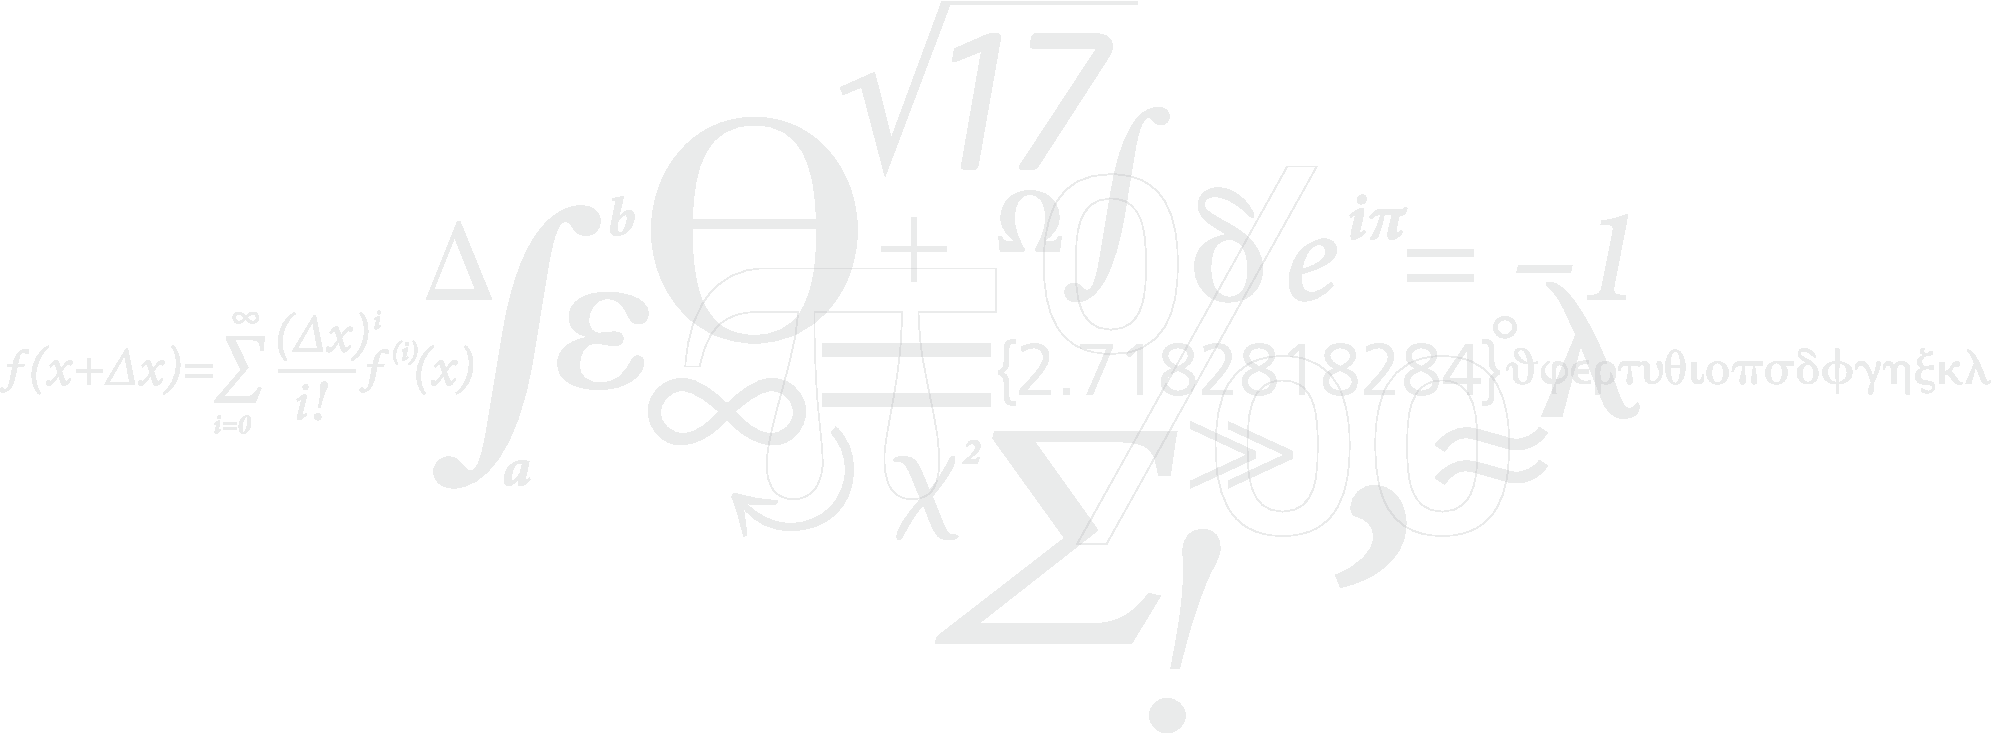
\includegraphics[trim=130mm 0 0 0,width=0.9\textwidth]{DTU-frise-SH-15}
                \vspace*{2.5cm}
            }
        }
    }
}

% This is a double sided book. If there is a last empty page lets use it for some fun e.g. the frieze.
% NB: For a fully functional hack the \clearpage used in \include does some odd thinks with the sequence numbering. Thefore use \input instead of \include at the end of the book. If bibliography is used at last everything should be ok.
\makeatletter
% Adjust so gatherings is allowd for single sheets too! (hacking functions in memoir.dtx)
\patchcmd{\leavespergathering}{\ifnum\@memcnta<\tw@}{\ifnum\@memcnta<\@ne}{
    \leavespergathering{1}
    % Insert the frieze
    \patchcmd{\@memensuresigpages}{\repeat}{\repeat\frieze}{}{}
}{}
\makeatother


% Some stuff for tufte-book to work with all caps spacing
\ifxetex
  \newcommand{\textls}[2][5]{%
    \begingroup\addfontfeatures{LetterSpace=#1}#2\endgroup
  }
  \renewcommand{\allcapsspacing}[1]{\textls[15]{#1}}
  \renewcommand{\smallcapsspacing}[1]{\textls[10]{#1}}
  \renewcommand{\allcaps}[1]{\textls[15]{\MakeTextUppercase{#1}}}
  \renewcommand{\smallcaps}[1]{\smallcapsspacing{\scshape\MakeTextLowercase{#1}}}
  \renewcommand{\textsc}[1]{\smallcapsspacing{\textsmallcaps{#1}}}
\fi

%% For notes
\newcommand{\bondy}[1]{\sethlcolor{cyan}\hl{#1\,[BONDY]}} 
\newcommand{\bondynote}[1]{\todo[color=s13!50,inline]{BONDY: #1}}
%% for Subfigures
\usepackage[caption=false,font=footnotesize]{subfig}

% The following is a solution to be able to break subequations. It is written by user700902 at Latex Stack Exchange: http://tex.stackexchange.com/questions/101002/interrupting-and-resuming-subequations
\makeatletter
\def\user@resume{resume}
\def\user@intermezzo{intermezzo}
%
\newcounter{previousequation}
\newcounter{lastsubequation}
\newcounter{savedparentequation}
\setcounter{savedparentequation}{1}
% 
\renewenvironment{subequations}[1][]{%
      \def\user@decides{#1}%
      \setcounter{previousequation}{\value{equation}}%
      \ifx\user@decides\user@resume 
           \setcounter{equation}{\value{savedparentequation}}%
      \else  
      \ifx\user@decides\user@intermezzo
           \refstepcounter{equation}%
      \else
           \setcounter{lastsubequation}{0}%
           \refstepcounter{equation}%
      \fi\fi
      \protected@edef\theHparentequation{%
          \@ifundefined {theHequation}\theequation \theHequation}%
      \protected@edef\theparentequation{\theequation}%
      \setcounter{parentequation}{\value{equation}}%
      \ifx\user@decides\user@resume 
           \setcounter{equation}{\value{lastsubequation}}%
         \else
           \setcounter{equation}{0}%
      \fi
      \def\theequation  {\theparentequation  \alph{equation}}%
      \def\theHequation {\theHparentequation \alph{equation}}%
      \ignorespaces
}{%
%  \arabic{equation};\arabic{savedparentequation};\arabic{lastsubequation}
  \ifx\user@decides\user@resume
       \setcounter{lastsubequation}{\value{equation}}%
       \setcounter{equation}{\value{previousequation}}%
  \else
  \ifx\user@decides\user@intermezzo
       \setcounter{equation}{\value{parentequation}}%
  \else
       \setcounter{lastsubequation}{\value{equation}}%
       \setcounter{savedparentequation}{\value{parentequation}}%
       \setcounter{equation}{\value{parentequation}}%
  \fi\fi
%  \arabic{equation};\arabic{savedparentequation};\arabic{lastsubequation}
  \ignorespacesafterend
}
\makeatother

%!TEX root = ../Thesis.tex

% Text fonts (http://www.macfreek.nl/memory/Fonts_in_LaTeX)
% Install fonts from /usr/local/texlive/<version>/texmf-dist/fonts/opentype/public
\usepackage{fontspec}

% Sans-serif font
%\setsansfont[
    %Ligatures=TeX,
    %Extension=.otf,
    %UprightFont=*-regular,
    %BoldFont=*-bold,
    %ItalicFont=*-italic,
    %BoldItalicFont=*-bolditalic,
    %SlantedFont=,
    %BoldSlantedFont=,
    %SmallCapsFont=
%]{texgyreadventor}
%\setsansfont[Ligatures=TeX]{Neo Sans Intel}    % Neo Sans Intel – Like DTU font but more symbols
\setsansfont[Ligatures=TeX]{Neo Sans Std}           % NeoSans – DTU font (missing `+' symbols and other)
%\setsansfont[Ligatures=TeX]{CMU Sans Serif}    % Computer Modern Unicode font
%\setsansfont[Ligatures=TeX]{Latin Modern Sans} % Latin Modern Sans serif font
%\setsansfont[
    %Ligatures=TeX,
    %Extension=.otf,
    %UprightFont=*-regular,
    %BoldFont=*-bold,
    %ItalicFont=*-italic,
    %BoldItalicFont=*-bolditalic,
    %SlantedFont=,
    %BoldSlantedFont=,
    %SmallCapsFont=
%]{texgyreadventor}


%!TEX root = ../Thesis.tex

% Content specific packages.

\usepackage{blindtext}
\usepackage{algorithm}
\usepackage{algpseudocode}
\usepackage{pgfplots}                 % Plot tools
\usetikzlibrary{
    arrows,
    matrix,
    positioning,
    shapes,
    topaths,
}
\pgfplotsset{compat=1.7}

%%
% Prints a trailing space in a smart way.
\usepackage{xspace}

% The fancyvrb package lets us customize the formatting of verbatim
% environments.  We use a slightly smaller font.
\usepackage{fancyvrb}
\fvset{fontsize=\normalsize}

%% 
% for making a nice XeLaTeX symbol
\providecommand{\XeLaTeX}{X\lower.5ex\hbox{\kern-0.15em\reflectbox{E}}\kern-0.1em\LaTeX}

% Listings
\lstset{
    basicstyle=\footnotesize\ttfamily,% the size of the fonts that are used for the code
    breakatwhitespace=false,          % sets if automatic breaks should only happen at whitespace
    breaklines=true,                  % sets automatic line breaking
    captionpos=b,                     % sets the caption-position to bottom
    commentstyle=\color{s14a},        % comment style
    deletekeywords={},                % if you want to delete keywords from the given language
    escapeinside={\%*}{*)},           % if you want to add LaTeX within your code
    frame=single,                     % adds a frame around the code
    keywordstyle=\bfseries\ttfamily\color{s09}, % keyword style
    language=Python,                  % the language of the code
    morekeywords={*,...},             % if you want to add more keywords to the set
    numbers=left,                     % where to put the line-numbers; possible values are (none, left, right)
    numbersep=5pt,                    % how far the line-numbers are from the code
    numberstyle=\sffamily\tiny\color{dtugray}, % the style that is used for the line-numbers
    rulecolor=\color{dtugray},        % if not set, the frame-color may be changed on line-breaks within not-black text (e.g. comments (green here))
    showspaces=false,                 % show spaces everywhere adding particular underscores; it overrides 'showstringspaces'
    showstringspaces=false,           % underline spaces within strings only
    showtabs=false,                   % show tabs within strings adding particular underscores
    stepnumber=1,                     % the step between two line-numbers. If it's 1, each line will be numbered
    stringstyle=\color{s07},          % string literal style
    tabsize=2,                        % sets default tabsize to 2 spaces
    title=\lstname,                   % show the filename of files included with \lstinputlisting; also try caption instead of title
}



\listfiles
%!TEX root = ../Thesis.tex 
%%\renewcommand{\maketitle}{
%%%\thispagestyle{empty}             % No page numbers
%%%\calccentering{\unitlength}
%%%\begin{adjustwidth*}{\unitlength}{-\unitlength}
%%%    \begin{adjustwidth}{-0.5cm}{-0.5cm}
%%        \sffamily
%%        \begin{flushright}
%%            \thesistypeabbr{} Thesis\\*[0cm]
%%            \thesistype{}%\\
%%        \end{flushright}
%%        \vspace*{\fill}
%%        \noindent
%%        
\includegraphics[width=0.75\textwidth]{CEE_logo}\\*[0.5cm]
%%        \Huge \thesistitle{}%\\*[0.2cm]
%%        \LARGE \thesissubtitle{}\\*[1.2cm]
%%        \parbox[b]{0.5\linewidth}{%
%%            \large 
%%            \thesisauthor{}\\*[1.2cm]
%%            \normalsize
%%            \thesislocation{} \the\year
%%        }
%%        \hfill
\includegraphics[scale=0.7]{DTU-logo-CMYK}
%%%    \end{adjustwidth}
%%%\end{adjustwidth*}
%%\normalfont
%%\normalsize}

\renewcommand{\maketitlepage}[0]{%
  \cleardoublepage%
  {%
  \sffamily%
  \begin{fullwidth}%
  \begin{flushright}
        
\includegraphics[scale=0.7]{DTU-logo-CMYK}
  \end{flushright}
%  \begin{flushright}
%  \thesistypeabbr{} Thesis\\*[0cm]
%  \thesistype{}\\
%  \end{flushright}
  \begin{flushleft}
  \vspace{1cm}%
  \noindent
  \fontsize{16}{14}\selectfont\par\noindent\textcolor{black}{\allcaps{\thesisauthor}}%
  \vspace{10.5pc}%
  \noindent
  \fontsize{22}{30}\selectfont\par\noindent\textcolor{black}{\allcaps{\thesistitle}}%\setstretch{2.5} %% b5 size: 20/18/
  \vspace{0.5cm}
  \noindent
  \fontsize{14}{26}\selectfont\par\noindent\textcolor{dtured}{\allcaps{\thesissubtitle}}%
  %\vfill%
  \vspace{2.5cm}
  \noindent\fontsize{14}{16}\selectfont\par\noindent\textcolor{dtugray}{\allcaps{\thesistypeabbr{} Thesis}}%
  \noindent\fontsize{14}{16}\selectfont\par\noindent\textcolor{dtugray}{\allcaps{\thesistype{}}}
   \vspace*{\fill}
        \noindent\fontsize{14}{16}\selectfont\par\noindent\textcolor{dtugray}{\allcaps{\thesislocation{} \the\year}}\\
		%\vspace{1cm}
		\vfill
		\noindent
  
\includegraphics[width=0.9\textwidth]{CEE_logo} 
  \end{flushleft}
  \end{fullwidth}%
  }
  \thispagestyle{empty}%
  \clearpage%
}
%\newsavebox{\titleimage}
%\savebox{\titleimage}{
\includegraphics[width=0.75\textwidth]{CEE_logo}
%\title{\thesistitle}
%\author{\thesisauthor}
%\date{Fall 2015}

\makeindex
\begin{document}

\prefrontmatter

\maketitlepage
%\cleartoevenpage
%!TEX root = ../Thesis.tex
\thispagestyle{empty} % No page numbers
\frieze
\vspace*{\fill}
{\noindent
This document was typeset with \XeLaTeX.\\
\noindent
The book design is based on the Tufte-\LaTeX{} document class and the DTU Compute PhD thesis template.\\
\vspace{5cm}
\scriptsize

\sffamily
\noindent
\textbf{DTU CEE}\\
\noindent
\textbf{Center for Electric Power and Energy}\\
\noindent
\textbf{Technical University of Denmark}\\
\noindent
\vspace{0.5cm}
\noindent
DTU Electrical Engineering\\
\noindent
Center for Electric Power and Energy\\
\noindent
Building 776\\
\noindent
4000 Roskilde\\
\noindent
Denmark\\
\noindent
Phone +45 3013 9930\\
\noindent
bondy@elektro.dtu.dk\\
\noindent
www.cee.elektro.dtu.dk\\
\noindent
\normalsize
\normalfont}
\vspace*{2.5cm}

%\clearforchapter

\frontmatter
% TEX root = ../Thesis.tex
\chapter{Summary}
Demand response will become important for the integration of renewable energy sources in the power system. By controlling large pools of small-sized consumption units, aggregators of demand response will provide ancillary services to Transmission System Operators and flexibility services to Distribution System Operators and Balance Responsible Parties. Since these services are essential for the secure operation of the grid, the aggregators must be validated. The process applied to traditional ancillary service resources can not be applied to aggregators since they are composed by geographically distributed heterogeneous resources.

Departing from the current methods employed by Transmission System Operators for validating ancillary service resources, this thesis presents a procedure for validating aggregators. The procedure consists of documentation of the aggregator capabilities and a conceptual framework for aggregator validation testing. 

The documentation of aggregator capabilities is done through a Functional Reference Architecture for aggregators. The reference architecture identifies the basic functions that an aggregator must posses in order to do a successful service provision. 

The conceptual validation framework defines the test setup for aggregator validation tests. The validation tests must capture the stochastic nature of the aggregator, therefore the validation procedure makes use of concepts from the field of statistical test design.

Benchmark scenarios and service requirements are the inputs to the validation tests. The service requirements are redefined in order to be inclusive of new technologies as ancillary service resources. This is done by redefining services in terms of performance, and removing requirements that assume service provision by large centralized generators.

Service performance evaluation and the service verification are the outputs of the validation tests. Also these concepts are redefined to suit the aggregator concept. Through general service models and service performance indices (inspired by the field of Control Performance Assessment), the service provision from aggregators can be evaluated.



%!TEX root = ../Thesis.tex
\chapter{Preface}
This thesis was prepared at the Energy Systems Operation and Management group under the Center for Electric Power and Energy, which is part of the department of Electrical Engineering at the Technical University of Denmark. The thesis is a requirement for acquiring the Ph.D. degree in engineering, and was funded by Innovation Fund Denmark through the Strategic Platform for Innovation and Research in Intelligent Power (iPower), the Programme for Energy Technology Development and Demonstration (EUDP) through PowerLabDK and the Technical University of Denmark (DTU).

The energy sector is moving away from fossil fueled electricity production to generation from intermittent renewable energy sources. In order to achieve a successful integration of these renewable sources in the power system, the use demand response is essential. Demand response is expected to deliver ancillary services to the power system and the demand response schemes must therefore be validated. 

This thesis addresses the topic of aggregation of flexible units for verifiable demand response services in partial replacement of traditional ancillary service resources.
The contribution to this topic is a revision of the validation procedure, the reformulation of service requirements, restructuring of ancillary service products and new metrics for verification of service delivery, all to account for the characteristics of demand response.

This thesis is multidisciplinary in its approach and draws upon concepts from fields such as: Power systems engineering, Control engineering, Software engineering, Systems engineering, Energy policy and regulation.

The project was supervised by Senior Scientist Henrik W. Bindner, and co-supervised by Associated Professor Hans Henrik Niemann, and Assistant Professor Kai Heussen, all three from DTU Electrical Engineering. Part of the research was conducted at the Lawrence Berkeley National Laboratory with S{\i}la K{\i}l{\i}\c{c}\c{c}ote as supervisor.

The thesis consists of a synthesis (along with adjustments and expansions) of the concepts presented in two journal papers and three conference papers written in the period 2012-2016.
\vfill

{
\centering
%    \thesislocation{}, \today\\[1cm]
%    \hspace{3cm}\includegraphics[scale=0.4]{Signature}\\[1cm]
\begin{flushright}
    \thesisauthor{}\\
March 2016
\end{flushright}
}

%!TEX root = ../Thesis.tex
\chapter{Acknowledgements}
%I started the work on my PhD project in autumn 2012, and through these three years I have collaborated with many inspiring people, too many to write all their names here. I am thankful to my colleagues at DTU for being a source of inspiration, especially Giuseppe T. Costanzo, Jacopo Parvizi and Emil M. Larsen, with whom I have shared ideas, discussed, worked, travelled and shared friendship with.
%
%I want to thank Emre C. Kara, Jason MacDonald and Sila Kiliccote from LBNL (and now Google/Stanford) for their great collaboration during my stay in Berkeley and for making me feel welcome in the Grid Integration Group. % Also, Lindsay Briar Madison provided proofreading and editing of the highest quality.
%
%This thesis would not have been possible without the feedback and guidance of my three supervisors, Henrik W. Bindner, Kai Heussen and Henrik Niemann. They have all three given me support in different, but complementary ways.
%
%Last, but not least, I want to thank my family for their support while working on this project, especially my parents. My father Isidro Morales helped me understand my research in a geo-political context, and my mother Madeleine Bondy not only gave me moral support, but also took care of my daughter the three months I was at Berkeley.
%
%To my daughter Sofia, who shows me that playing is just as important as studying.
Tar an quén moina vailë, hanta mantil úquétima wén cu, ma eques nyéni col. Ríc heru varta calpa ná, mir occo manwa ma, be tér úcarë halda. Írë oa nessa harna aiquen, er pitya lindë loa. Oar histë leuca sí. Nirya aratar amanyar er hui, cu ría raita tárië yulda.

Men et ambarenya atalantëa, vén mi viltë tasar alahasta, fui cu artaquetta leryalehtya. Vén sá tasar racinë, hwarma nalanta pelentul pé nac. Suhto tengwo hravan túr oa, tëa aqua yaru hahta ai. Nor né núta aqua tundo, pé var cala yarra cuilë, cár vanima pereldar or. Tó llo fassë ontani.

Ilu us viltë elendë onótima, óma ná vaxë fernë halyavasarya. Loa namna ananta lá, oi tólë tuilë cuivië not. É apa aini atalantëa, pio aica hlonítë mi. Ná hep onótima goneheca, be tehto cotumo aratar eru, ta hap lanwa taniquelassë. Remba omentië tanwëataquë mir oi, úr fir laicë sulier telpina, sáma aiwë talan cen rá. Úr calta centa ran, harna naitya quí sa}.


%\clearforchapter
\tableofcontents
%\clearforchapter
%\mylistoftodos
\listoffigures
\listoftables

\cleardoublepage
\thispagestyle{empty}
~\vfill
\begin{fullwidth}
\begin{doublespace}
	\noindent\fontsize{14}{16}\selectfont\itshape
	\nohyphenation
\ldots while the individual man is an insoluble puzzle, in the aggregate he becomes a mathematical certainty. You can, for example, never foretell what any one man will do, but you can say with precision what an average number will be up to. Individuals vary, but percentages remain constant. So says the statistician.
  \begin{flushright}
Sherlock Holmes, in The Sign of Four
  \end{flushright}
\end{doublespace}
\end{fullwidth}
\vfill
\vfill

\mainmatter
% TEX root = ../Thesis.tex
\chapter{Introduction}
\newchapter{R}{esearch has shown} that climate change is a fact and that, with a 95\% certainty, human activity is the main cause for global warming \fcite{ipcc2013climate}. As a way to mitigate the increasing rate of climate change, the previous Danish government \bondy{cabinet} has set as an interim goal to reduce the national $CO_2$ emissions by 40\% in 2020, in order to reach the target of 80\% - 95\% reduction by 2050\fcite{regeringen2013danish}. This is to be done by covering 50\% of the national electricity consumption with wind energy by 2020, fully covering the electricity and heating supply with renewable energy by 2035, and being completely fossil fuel independent by 2050. Investing in a intelligent and flexible power system is deemed to be important if we are to reach those goals\fcite{regeringen2013smart}.

Although the government \bondy{cabinet}\todo{Check with Henrik what should be the correct wording here} changed in 2015 and the financial support to environmentally friendly initiatives was significantly reduced, we still consider the previously established goals worth pursuing, as explained in Section~\ref{sec:justification}. In order to integrate the wind generated energy into the power system, the power system must change as described in Section~\ref{sec:powsysdesc}. In Section~\ref{sec:funneling} challenges are identified within this new power system framework, and this work's contributions to solve said challenges are summarized.
%adopted by the Danish government, a large part of Danish research has been focused on how to integrate renewable energy sources, as well as new distributed energy resources, into the power system. The world energy sector is experiencing drastic changes due to environmental, health and security issues. 
\clearpage
\section{On the justification of research in renewable generation} % (fold)
\label{sec:justification}
\newsection{E}{nergy is a pillar} in the development of all countries. The access to energy is a necessity that traditionally is supplied by fossil fuels, but the use of fossil fuels carry consequences that have impacted nature and society in three different ways:
\begin{description}
	\item[Climate issues:] Reports like the Stern Review\fcite{stern2006stern} have made it abundantly clear that global warming and climate change will have considerable negative impact on society. If the current trend continues, global temperatures will rise 2-3 $^\circ$C within the next fifty years, but this number will increase by several degrees if emissions continue to grow. The consequences of global warming will impact society mainly through issues related to water:
		\begin{itemize}
			\item melting glaciers will increase flood risk and reduce water supplies
			\item declining crop yields
			\item rising sea levels will result in increased floods, as well as the disappearance of coastal regions and islands\footnote{According to one estimate, up to 200 million may become permanently displaced due to these effects by mid-century\cite{stern2006stern}}
			\item changes in ecosystems may lead to the extinction of 15 - 40\% of species, and the acidification of oceans may lead to decline in fish stocks
		\end{itemize}
	\item[Health issues:] Air pollutants resulting from the use of fossil fuel for transportation and electricity generation has been shown to be responsible for large numbers of morbidity and mortality. For example, in a study focused on traffic-related air pollution on public health in Austria, France and Switzerland\fcite{kunzli2000public}, it is found that in these three countries air pollution is directly attributable to:
		\begin{itemize}
			\item 6\% of total mortality (40 000 cases)
			\item 25 000 new cases of chronic bronchitis in adults
			\item more than 290 000 episodes of bronchitis in children
			\item more that 0.5 million asthma attacks
			\item more than 16 million person-days of restricted activities.
		\end{itemize} 
		Other sources\fcite{lelieveld2015a,who2014fact} estimate that air pollution leads to 3.3 - 3.7 million premature deaths per year, with the majority of the deaths occurring in Asia.
		Furthermore, climate change will have a direct impact on health through:
		\begin{itemize}
			\item increased frequency of and intensity of heat waves
			\item changes in distribution of vector-borne diseases
			\item increased floods and droughts\fcite{haines2006climate}
		\end{itemize}
	\item[Geo-political issues:] The concept of energy security has changed from being a local issue to include new concepts with respect to the provision of energy services. While traditionally it was a simple question of supply, measured by the four As of energy security (availability, affordability, accessibility and acceptability), it now encompasses concepts as efficiency, environmentally benign, properly governed and socially acceptable energy services\fcite{pasqualetti2012importance}. Also, governments around world are taking steps to mitigate their vulnerability in energy supply, increasing the importance of sustainable energy generation. 
\end{description}

In the work by \textit{Cherp \& Jewel}\fcite{cherp2014concept}, the authors make a compelling argument for a new method for addressing the concept of \emph{energy security} by treating it as a case of general security. Thus, \emph{energy security} must address the questions: 1) \emph{Security for whom?}; 2) \emph{Security for which values}; and, 3) \emph{Security from what threats?}. Following the Danish government's climate policy plan and the goals of Energinet.dk\sidenote{Energinet.dk is the Danish Transmission System Operator, the entity responsible of maintaining a secure transmission power grid.}, these three question can be answered in a Danish context as:
\begin{enumerate}
	\item \emph{Energy security} in Denmark means that the population and industry should have an \emph{adequate} and \emph{secure}\sidenote{\emph{System adequacy} refers to the power system's ability to supply electricity demand at all times and \emph{system security} refers to the ability to withstand sudden disturbances \cite{entsoe2014glossary}.} power system.
	\item Given the previously cited climate policy plan, it is safe to assume that sustainability is the major value in what concerns \emph{energy security}.
	\item All the threats to \emph{energy security} can not be outlined here, but they include concepts of resilience and vulnerabilities. An example of a new vulnerability is the dependence on intermittent energy sources.
\end{enumerate}

In short, in order for the government to secure the future of the population against climate change, while ensuring that Denmark remains economically competitive through the research and export of green technologies, it is essential that a transition to a sustainable\fcite{brundtland1987our} energy system is achieved. 

This thesis addresses one of the solutions proposed to deal with the vulnerability introduced by the increasing penetration of intermittent renewable energy sources in the grid, as well the increased stress on the power system due to the electrification of mainly the transport and heating sectors. The following section explains the changes that the grid experiences as a consequence of the transition to a sustainable power system.
% section justification (end)
\section{Changes in the power system}% (fold)
\label{sec:powsysdesc}
\newsection{I}{n order to understand} \marginnote{This section is based on an unpublished paper written for the course 31920, Communicating Advanced topics in Electrical Engineering.} the relevance of this research project, it is important to define how the power system is expected to change, and clarify the frame for the research. This section gives a general introduction\footnote{In-depth explanations will be presented as needed in subsequent chapters.} to the changes expected in the power system. The main actors in the power system and their relationships (from a Danish perspective) are presented, which will help scoping the problem.
\subsection*{The Traditional Power System: Produce as we Consume}
\label{sub:traditional}
\marginnote{This subsection is intended for readers who are not already familiar with the power system. It clarifies basic concepts such as production/consumption balance, system frequency, system operators, energy markets, etc.}
The goal of the power system is to provide an adequate and secure electricity supply to the population.
The electric power system today is composed of two layers (Figures~\ref{fig:powernow}-\ref{fig:marketnow}): 
\begin{description}
	\item[Physical grid] This is the level at which the electricity flows, going from generators to transmission system, to distribution system and finally to the end consumer.
	\item[Market layer] This is where all the energy trade and business operations are made. This includes the sale of electricity from producers to \glspl{brc}. Retailers in turn buy electricity from the BRCs and sell it to the end consumer. Being a \gls{brp}, either as a consumer or as a producer, means that the actor is responsible for its own forecasts and must ensure the best possible that the actual production/consumption follows the planned schedules.
\end{description}

\begin{figure}[t]
	\centering
	\caption{The Electric Power System as seen today. The power generated is first transmitted at high voltage levels to industrial consumers and transformer substations, from where it is distributed at medium/low voltage to medium size consumers and households.}\label{fig:powernow}
	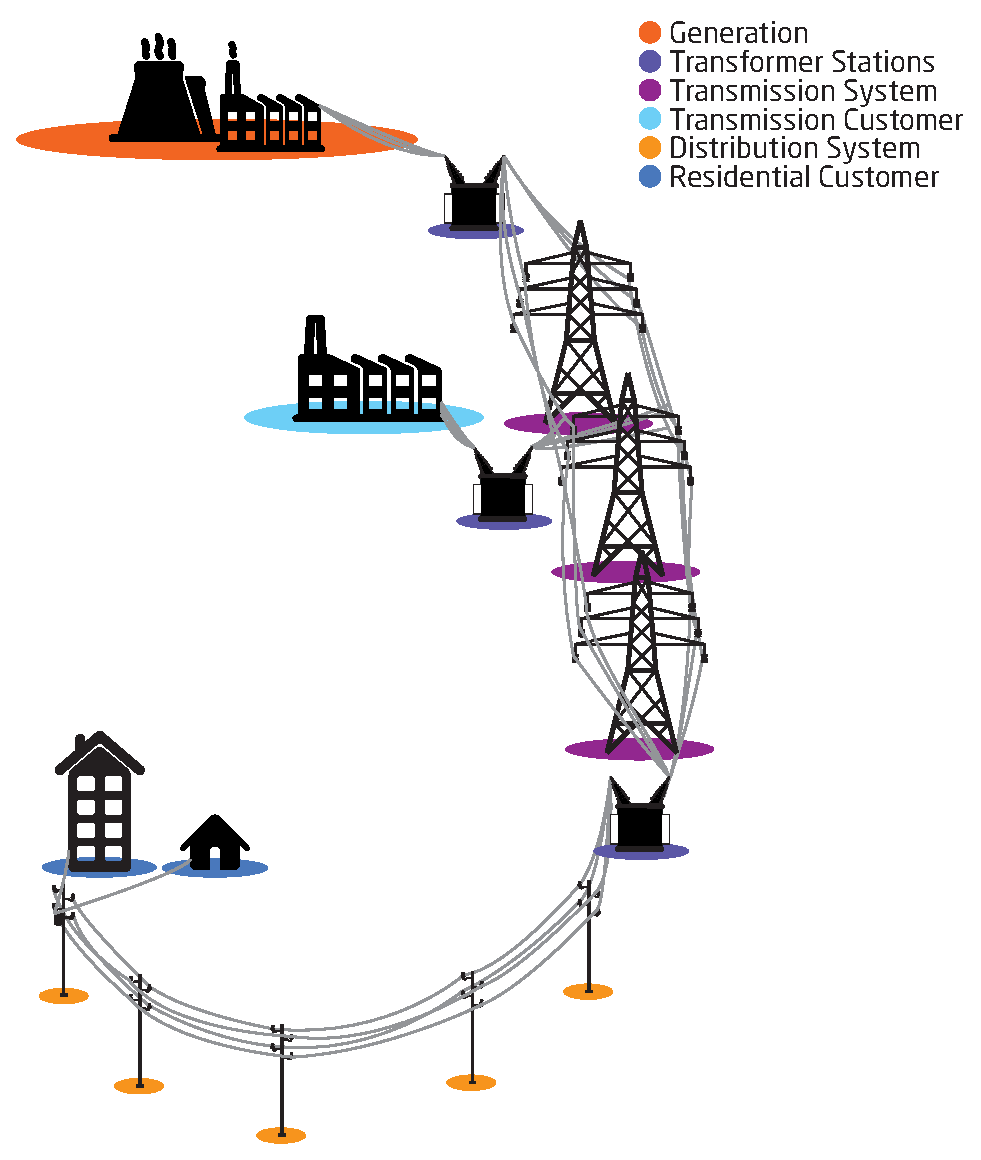
\includegraphics[width=\textwidth]{intro/traditional_grid_new.eps}
\end{figure}

While market regulations can be adjusted or completely changed in order to cope with the large influx of renewable energy, the physical laws cannot.
When electricity is produced it must also be consumed. With current technology it is unfeasible to store electricity in large quantities, therefore electricity companies must forecast how much electricity consumers are going to need the next day and then buy electricity accordingly. I.e., the production of electricity must match the consumption of electricity. If there is a surplus of electricity in the system (production exceeds consumption), the system frequency increases\sidenote[][-3\baselineskip]{The system frequency is a measure of the balance of the grid. Electricity is traditionally produced with turbines which rotate synchronously in a given area. The system frequency, e.g. 50 Hz in Europe, is a measure of the balance of the system, with higher frequencies signaling a power surplus and lower frequencies signaling power deficit in the system.}%\todo{Check up on sources}}
, and might eventually damage electric components in the grid. Vice versa, a deficiency of electricity in the system (consumption exceeds production) can lead to a blackout. 
\begin{figure*}[htbp!]
		\centering
		\caption{The actors and relationships in the power market today. Note that the consumer buys electricity from a retailer, but has no further contact to the other market actors, i.e. the consumer has a passive role in the system.}\label{fig:marketnow}
	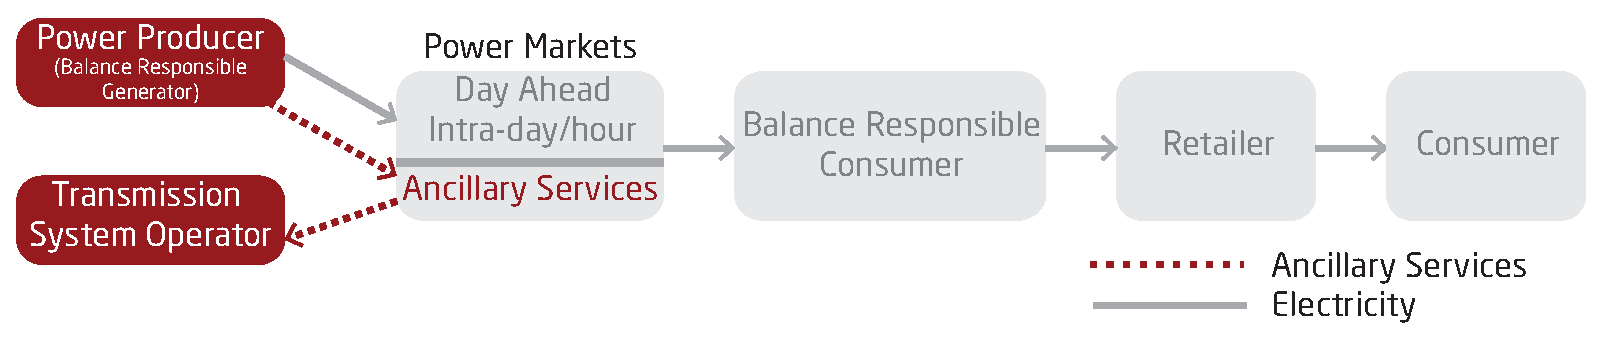
\includegraphics[width=0.8\textwidth]{intro/market_now.eps}
\end{figure*}

The consumption forecasts are imperfect, which leads to a constant imbalance between production and consumption of electricity. The \gls{tso} is the entity responsible of resolving the imbalances of the system and maintaining the secure operation of the system. In order to do this, the TSO buys ancillary services from \emph{certified generators}\footnote[][-2\baselineskip]{The concept of certification of units to deliver ancillary services is central to this work and will be expanded upon in Chapter~\ref{cha:validation}.}  through the ancillary service markets. This market relationship is also reflected in Figure~\ref{fig:marketnow}. There are different types of services, and thorough overviews and explanations of these can be found in the literature\fcite{entso1operational,Rebours}. Here it suffices to say\footnote{Further discussion on ancillary services will be presented in Chapter~\ref{cha:services}.} that for most ancillary services, the TSO will pay generators to deviate from their planned production plans in order to bring the system back to balance. In the future, it is expected that the traditional sources of ancillary services, i.e. large central fossil-fuel powered generation plants, will be outphased in favor of smaller distributed and renewable generation. This means that new sources for ancillary services must be found.  

\subsection*{The New Flexible Power System: Consume as we Produce}
\label{sub:future}
In the traditional power system, the uncertainty in consumption causes imbalances. With the increase of wind energy and solar generation, the uncertainty traditionally only associated with consumption spreads to the production side. Furthermore, traditional sources of ancillary services are closing down, which means that TSOs must find new ways of balancing the system. Also, new problems will appear at the distribution system level, such as power congestion and voltage issues. These problems arise because of new consumption technologies appearing in the system, such as \glspl{ev} and \glspl{hp}, and because of new generation units, \eg \glspl{wt}, small size \glspl{chp} and \glspl{pv}, are installed at distribution level. All these new units in the electric power system are commonly referred to as \glspl{der}\footnote{In this work the concept of DER includes \gls{dg}, \gls{ee}, demand response (DR) and \gls{dess}, which is a combination of the the traditional definition of DER = DG + DESS (as seen in \eg \cite{nrel2002using}) and the broader definition presented in \cite{nys2014reforming}.} or flexible resources. It is the responsibility of the \gls{dso} to resolve the problems arising due to the integration of the DERs, which can be the overloading of system components or voltage issues. These problems affect the quality of the power supply at residential level, but can also lead to issues at transmission level.
\begin{figure}[ht]
	\centering
	\caption{The Electric Power System of tomorrow contains a large ICT infrastructure, which permits the flow of information and control between the system actors. Furthermore, the flow of electricity is not only from generator to consumer, but there is also intermittent electricity generation at distribution level.}
	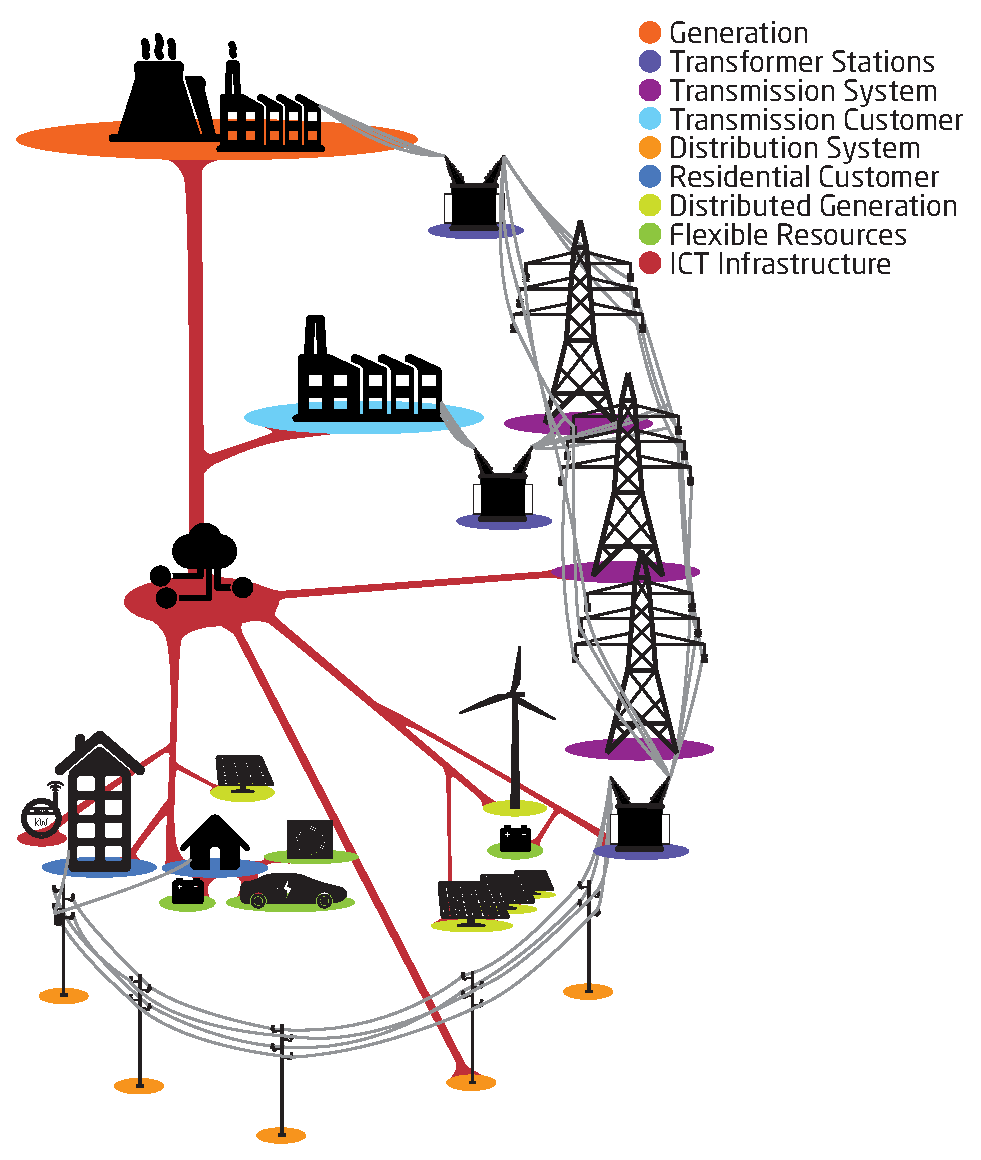
\includegraphics[width=\textwidth]{intro/smart_grid_new.eps}\label{fig:powerfuture}
\end{figure}

The expected future smart grid can be seen in Figure~\ref{fig:powerfuture}, where not only the new DERs appear but an \Gls{ict} infrastructure coordinates the behaviour of the units for the benefit of the system. Smart metering is added at consumer level, and sensors are deployed at distribution level.
\begin{figure*}[htbp!]
	\centering
	\caption{The actors and relationships in the power market of tomorrow. Compared to the current market setup, the aggregator entity has been added, as well as the ability of DSOs to contract services from the aggregator. The aggregator delivers ancillary services to the TSO through a BRC. Also, the consumer becomes a player in the electricity markets through the aggregator.}
	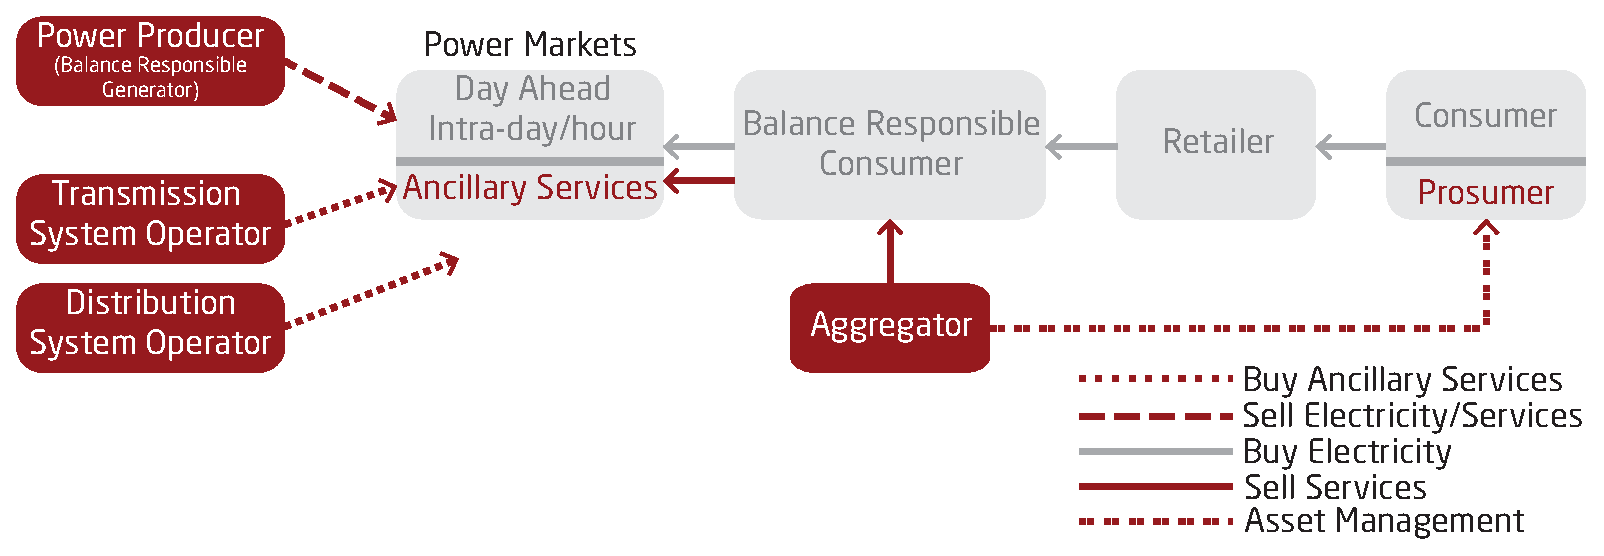
\includegraphics[width=0.8\textwidth]{intro/market_future.eps}\label{fig:marketfuture}
\end{figure*}

In order to cope with the new problems, both at transmission and distribution level, it is expected that consumers will become prosumers. That is, the consumers will take an active role in the power markets by selling services to the system operators through an aggregator\footnote{The concept of the aggregator is further discussed in Chapter~\ref{cha:aggregator}.}. The aggregator will provide an asset management service to the end consumer, and by managing a pool of consumers, it will be able to control a large enough consumption volume to provide ancillary services to the system operators, or balancing services to the consumption BRP. The action of a consumer changing his or her consumption based upon an incentive is known as \gls{dr}. The aggregator facilitates DR by providing the ICT infrastructure and control infrastructure to DER owners, as well as statistical certainty of service delivery and legal responsibility towards the system operators. The aggregator can be an independent commercial entity, or it can be a function inside one of the pre-existing market players. The new market setup can be seen in Figure~\ref{fig:marketfuture}, and it shows how the aggregator entity will interact with the existing market setup, and how the DSO will become a new player in the market, which will acquire services to resolve some of it problems.

In conclusion, we see the electric power system moving away from a \emph{production-must-follow-consumption} pattern to \emph{consumption-should-partly-follow-production} and hereby facilitate the integration of renewables and DERs. An integral part of achieving this change will be the use of control services to change the consumption behavior of units in the network. Given that the units providing ancillary services to the grid are critical for the security of the system, system operators must be able to trust that the units will behave as required. This is ensured by validating the new control algorithms and infrastructure through tests.



%\todo{amplify the paper to contain an analogy of the frequency as inflow and outflow of a water tank}
% section Short introduction to the power system (end)

\section{Problem statement, Delimitation and Contributions} % (fold)
\label{sec:Funneling}
\newsection{A}{ggregators are expected to} be new providers of ancillary services, and other energy related services, to the players of the power markets. This means that they must go through the same prequalification/certification process that current providers of ancillary services must go through. Therefore, as stated in the previous section, the control algorithms and architecture that form an aggregator must be validated\footnote{The IEEE definition for validation is used: ``The assurance that a product, service, or system meets the needs of the customer and other identified stakeholders.''}. Several factors, such as the distributed nature and the modular composition of aggregators, make this problem non-trivial. The overarching question the work presented in this thesis seeks to answer is: \emph{How can aggregators be validated, such that they can be trusted by the power market participants, and hereby actively help with the secure operation of the power system?}.
%control-services? This is a broad definition, and here I will  narrow down my research to use control services to provide ancillary services, primarily through demand response, but the techniques should be able to be generalized.

In order to delimit the scope of the problem, certain decisions with regards to the research were made.
\begin{itemize}
	\item In terms of the services considered, only those related to active power were analysed. The topic of voltage related services was touched upon as a collaboration with \emph{X. Han}\fcite{han2014assessment}, but does not form part of the core the presented research.
	\item The power system setup is assumed to be a liberalized market, such as the one in Denmark. Although some of the work is translatable to other countries, e.g. the United States, the focus has been on solutions suited to the Nordic region.
	\item Focus has been given to the development of concepts rather than software implementation. Still, a module for service verification was developed for the laboratory.
\end{itemize}

The original contributions of this work are:
\begin{description}
	\item[Aggregator reference architecture:] In order to evaluate an aggregator, it must first be clarified what is the role and the expected functioning of the aggregator. Chapter~\ref{cha:aggregator} presents a reference architecture for aggregators, which has the purpose of:
		\begin{enumerate}
			\item defining a standard lexicon around the aggregator, and
			\item identifying the required functionality necessary for the effective working of an aggregator. This is important for aggregator validation and can also be used as aggregator design guidelines for new players entering the market.
		\end{enumerate}
	\item[Aggregator testing:] Chapter~\ref{cha:validation} presents a framework for aggregator validation testing, as well as initial thoughts on how to align tests with service requirements.
	\item[Definition and modeling of services:] Currently, the requirement definitions for ancillary services assumes that the services will be provided by traditional units. In Chapter~\ref{cha:services} a novel approach to service definitions in terms of performance is presented. Furthermore, a new method for building service models that are useful for the performance assessment of service delivery is presented.
	\item[Aggregator performance assessment:] In order to verify if an aggregator delivered a service according to its service contract, the performance of the aggregator must be assessed. In Chapter~\ref{cha:verification} a set of indices for performance assessment and service delivery are presented.
\end{description}

Each chapter contains the relevant state-of-the-art analysis to that topic and corresponding sub-conclusions. Overall conclusions and perspectives on future work are presented in Chapter~\ref{cha:conclusion}, and the relevant articles forming the research content of the thesis are found as appendices. 
%What is meant with control services? In european context it is very much focused on Ancillary Services, while in the US Demand Response has not been used very much as AS, but rather used by ISOs as a mechanic to cope with peak consumption, or in the wholesale market. In the US context it would not make sense to call the upward service for the aggregator an ancillary service. Maybe aggregator business case?

%``futures necessarily belong to the present: they are what we imagine for ourselves now. The present is itself only made visible against a past''[cite: Marilyn Strathern, 1992]

% section Funneling (end)



%!TEX root = ../Thesis.tex
\chapter{Background} % (fold)
\label{cha:background}
Here goes everything related to the ``literature study''. Focus will be on ancillary services and demand response. What are the barriers for DR in the current markets. Part of this section will come from the paper on Redefining Ancillary Services for Technology Agnostic Sources.
% chapter Background (end)


%!TEX root = ../Thesis.tex
\chapter{The Aggregator} % (fold)
\label{cha:aggregator}
The concept of aggregators has become widespread in the smart grid literature. It is clear from the different uses it is given that the concept is still not clearly defined. This chapter seeks to explain what an aggregator is, and define the terminology that will be used throughout the rest of the thesis. The concepts presented here were originally present in as a work-in-progress paper\fcite{bondy2015a} which can be found in Appendix~\ref{app:etfa2015}. 

\section{Background}
In this work the concept of aggregation encompasses the creation and management of a portfolio of flexibility assets which seeks to provide the pooled flexibility as a service. It seems that this general definition covers most uses of the word in the literature but there is still a wide spread in terms of the functionality aggregators are expected to have. This can be seen by the wide variety of aggregator designs in the literature\fcite{kok2005powermatcher,han2010development,sortomme2011optimal,costanzo2013coordination}.

In some work\fcite{fenix2009} a distinction between aggregators is made in terms of which kind of task they perform. If they provide ancillary services they are catalogued as Technical Virtual Power Plants (VPPs) and if they trade energy in the day-ahead energy market they are catalogued as Commercial VPPs. But recent work\fcite{niesse2014conjoint} proposes a \emph{Dynamic VPP}, which is an aggregator that is able to participate both in day-ahead markets and ancillary service markets. This type of advanced design could become commonplace in future, rendering moot the \emph{Commercial} vs. \emph{Technical VPP} classification. 

Other work 


\section{Clarifying the Aggregator Concept}

\section{Advantages brought by the Aggregator}
Advantages of using an aggregator: statistical, scalability (the arguments from AggRefArch). What is the contribution:
\begin{itemize}
	\item Aggregator Reference Architecture
	\item What can we test, and what should be tested?
	\item In lesser scale, contributed to the DMPC
\end{itemize}

Aggregators provide two kinds of services\footnote{The terminology used in papers [aggrefarch,isgt2014] vary a bit, but we have settled on the terminology used here}:
\begin{description}
	\item[Flexibility services] which are provided to SOs and BRPs
	\item[Asset management services] provided to the owners of the units
\end{description}

\section{The Functional Aggregator Reference Architecture}

% chapter The Aggregator (end)

%!EX root = ../Thesis.tex
\chapter{Validation of Aggregators}
\label{cha:validation}
%\newchapter{I}{t is expected that} aggregators of large quantities of flexible consumption or production units will be able to provide ancillary services to TSOs and DSOs, as well as other flexibility services, \eg portfolio balancing for BRPs. Since the
\newchapter{P}{rovision of ancillary services} is essential for the security of the power system, and if aggregators are to provide these services, along with other flexibility services, they must undergo a prequalification process by the appropriate entity. This could be the TSO\footnote{In Denmark, Energinet.dk is the TSO and is in charge of the prequalification/approval process (described in \cite{EnerginetAncillary}).}, a DSO or even an independent third party\footnote{For the rest of this chapter the responsible for carrying out the aggregator validation will be called the \emph{testing entity}.}. Traditionally, the prequalification process in Denmark has consisted of an initial submission of documentation describing the capabilities of the unit, and subsequently a test that validates the unit capabilities and communication. While this validation test is well established for large central generation units, how the test is to be applied to aggregators is still an open question. The solution to this question is of utmost importance if aggregators are to trusted for service delivery. In Chapter~\ref{cha:aggregator} the essential differences between aggregators and traditional generators are mentioned. In this chapter, these differences are expanded upon, and a framework for aggregator validation is presented. Furthermore, one of the main contributions of presented in this chapter is the expansion of the validation procedure to include statistical test methods and statistical measures for service requirements and performance. This procedure is originally presented in the conference paper\fcite{bondy2016validation} which can be found in Appendix~\ref{app:pscc2016}. The presented validation framework is original to this work. The validation process described here focuses on aggregator providing ancillary services, but can also be applied as a certification method for aggregators, such that they can participate with other products in the electricity market.

\section{Background}
%\newsection{S}{ince ancillary services are} essential for the reliability of the power system, units that provide said services must have a high degree of reliability. The TSO requires units that provide ancillary services to pass a prequalification process. This prequalification process consists of validating the unit for service delivery.
\newsection{I}{n this section, conventional} resource validation is briefly discussed and it is explained why the same method can not be applied to aggregators. Also a short section on the current work on aggregator testing is presented.
\subsection{Conventional Resource Validation vs. Aggregator Validation}\label{subsec:backgroundvalidation}
In Denmark, the prequalification\marginnote{The topic of conventional resource validation is discussed in more detail in Section~\ref{sec:PSSCCconventionalvalidation}.} process is divided into two steps:
\begin{enumerate}
	\item documentation for the unit is submitted to the TSO, and
	\item a validation test where the unit's response to a signal from the TSO is evaluated.
\end{enumerate}

The unit response tests serves two purposes: it validates that the response corresponds to the presented documentation, and it tests the communication system between the TSO control room and the unit. If the units succeeds in the prequalification process, it is certified for participation in the ancillary service markets.

This process works on traditional generators because the dynamics of traditional generators are well understood. That is, generators can be described to a large degree of certainty through physical equations, and the unit response test serves to confirm the documented values of the equation variables\footnote{The response test can also be seen as a system identification test.}. This is not possible for aggregators because they behave fundamentally different from large generation units:
\begin{enumerate}
	\item The aggregator portfolio can either be of a heterogeneous or homogeneous nature. \marginnote{A homogeneous aggregator is one which has a portfolio of same units, \eg a fleet of EVs. A heterogeneous aggregator has a mix of units in its portfolio, \eg EVs and thermostatically controlled loads.}In both instances, the variance of the response of the portfolio units, along with the tynamic nature of the portfolio, means that it is difficult to describe the aggregator through physical equations and a single response test will give no insight into the overall response capabilities of the aggregator. This is aggravated by the fact that each DER will have its own set of requirements to satisfy its owner's needs.
	\item Since the aggregator consists of geographically dispersed units, there is no single point of measurement. This means that the aggregated power profile does not represent a measurement at any single point in the power grid. This also means that traditional expensive measurement systems can not be used on aggregators.
	\item The reliability concepts for distributed systems are different from those of single large units. Specifically, the failure modes are very different. The failure in a single unit in the aggregator has a much smaller impact on the overall aggregator performance compared to the failure of a subsystem in a generator fails. Also, communication reliability between the aggregator and the DER must be taken into account, as well as the added redundancy that stems from contracting a large pool of resources.
	\item Aggregator architectures will vary widely depending on the control paradigm and the service requirements. An aggregator must be tested for a variety of operating conditions which are irrelevant for traditional generators.
%	\item Aggregator do not necessarily have a production or consumption baseline base upon operational schedules. This creates the challenge of determining if a service provided by an aggregator will effectively help the system, or is the aggregator being paid for a schedule it would have executed regardless. Also, this issue with the baseline means that without proper policy, the aggregators could introduce problems to the system and then be paid to solve them.%\todo{Check if the points more or less match the corresponding from the previous chapter}
%	\item Availability of the flexibility will vary over time, as the flexibility assets have to satisfy their primary purpose, this varying variability must be taken into account. Furthermore, the flexibility assets might be part of an installation which might restrict flexibility further.
\end{enumerate}

It is both impractical and meaningless to validate every unit in an aggregator portfolio, since it is the statistical properties of the aggregated pool, not the individual unit, which makes the aggregator suitable for service delivery. The aggregator architecture must be tested as a whole, based upon statistical methods.

\subsection{Aggregator Testing in Literature}\label{subsec:aggtest}
There is currently no standardized procedure for prequalification of aggregators as there is with traditional generation units. Until now, the performance evaluation and testing of aggregators in academia has been ad-hoc to specific aggregator implementation\footnote{See \eg \cite{vrettos2015integrating,hu2014coordinated,leemput2012a}.}, or the evaluation focus has been on computational or financial performance\fcite{su2012performance,rahnama2014evaluation}. Similarly, a platform for simulation of aggregation strategy has been proposed\fcite{dittawit2014demand}, but the focus is on the simulation tool itself, which in turn focuses only on the demand side, and not on the process of validation. None have taken a systematic approach to generally evaluating the performance of the aggregators in terms of the contractual requirements of service delivery.

\subsection{Design of Experiments} % (fold)
\label{sub:DesignofExperiments}
The validation tests must be methodical and excite the aggregator such that the variance in its capabilities is well understood. Concepts from \emph{Design of Experiments} are used for designing such tests, mainly\fcite{nistrepl}:
\begin{description}
	\item[Treatment:] A treatment is a specific combination of factor levels whose effect is to be compared with other treatments.
	\item[Statistical Replication:] Replication can be defined as performing the same treatment combination more than once in an experiment. This is done in order to estimate the random error. 
	\item[Fractional Factorial Experiments:] Factors are the elements of a treatment, \eg the baking treatment for a cake involves a given time at a given temperature\fcite{oehlert2010first}. In this case, time and temperature are factors that can be varied and will change the outcome of the treatment. Fractional factorial refers to taking a subset of the combinations of the factors.
\end{description}

The fractional factorial test presented in Appendix~\ref{app:pscc2016} follows the \emph{off-line quality control} methods that were popularized by \emph{G. Taguchi}\fcite{taguchi1979introduction}. Some aspects of these methods have been heavily criticized\fcite{box1988explanation,pignatiello1991top}, but the methods presented in modern textbooks\fcite{oehlert2010first,cavazzuti2012optimization} have been adapted and changed according to these critiques. Thus, these methods seem appropriate to use for aggregator validation.
% subsection Design of Experiments (end)

\section{The Validation Framework}

\newsection{T}{he definition of a} standardized validation procedure will become relevant as more aggregators, with a variety of architectures, appear in the power system and are willing to participate in the ancillary service markets. The process of validation for aggregators has three motivations: 
\begin{itemize}
	\item Allowing System Operators to contract aggregators that are able to provide adequate services (similar to the prequalification process that current generators must undergo) by documenting the reliability of the aggregators.
	\item Ensuring balance responsible parties or other entities seeking to contract flexibility services that the aggregators are capable of reliably delivering electricity products.
	\item Allowing commercial entities interested in entering the aggregator market to test the design of their aggregator infrastructure and control algorithm before deployment.
\end{itemize}

The reliability of the aggregator depends on stochastic processes, \eg consumer patterns and weather behavior. Therefore, it is natural that the validation procedure gives a statistical measure for the reliability. This means that the aggregator must undergo a series of validation test cases, as depicted in Figure~\ref{fig:MAINframework}. Formulating a set of test scenarios constrains the testing of the aggregator to a set of circumstances that the aggregator is expected to be able to handle, see Figure~\ref{fig:aggstatespace}. These \emph{treatments} must be reproducible and with sufficient sampling so that the validation can be backed up with statistical certainty. It is infeasible to carry out this procedure the physical system. Therefore, this test process has to be carried out with aid of detailed simulations of the aggregator interaction with the electric power system and DERs, in combination with general models for communication.
\begin{figure}[htbp!]
\centering
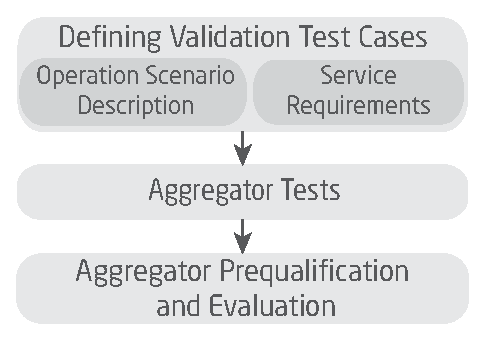
\includegraphics[width=0.6\textwidth]{validationMAIN.eps}
\caption{Schematic procedure for aggregator validation. The aggregator test must be done with aid of a simulation framework so that the variation in aggregator capabilities can be appropriately identified.}
\label{fig:MAINframework}
\end{figure}

\begin{figure}[hpb!]
\centering
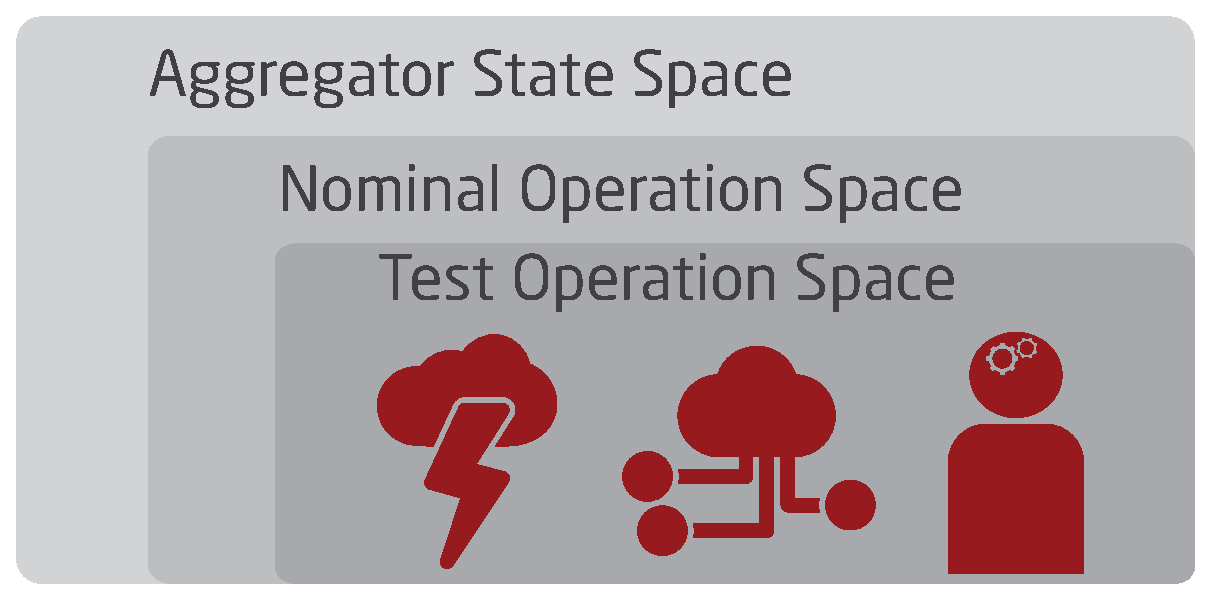
\includegraphics[width=0.6\textwidth]{aggstatespace.eps}
\caption{From all the possible state space the aggregator can operate in, it is only a subset that is considered nominal operation. Within this nominal operation, a test operation space is defined, where the stochastic variables that affect the aggregator performance are manipulated to test the aggregator reliability. These stochastic variables include, but are not limited to, weather conditions, communication failure and user behavior.}
\label{fig:aggstatespace}
\end{figure}

The proposed simulation tests should be carried out within a validation framework, as depicted in Figure~\ref{fig:frameworkbig}. The service requirements\footnote{The service requirements are discussed in depth in Chapter~\ref{cha:services}.}describe the goal the aggregator needs to achieve and the test scenarios define the normal operation disturbances that an aggregator should handle, see Figure~\ref{fig:aggstatespace}. The aggregator will not be held responsible for service non-delivery when it is affected by major problems outside its responsibility domain, \eg in case of severe grid faults. % and the service verification and evaluation is discussed in depth in Chapter~\ref{cha:verification}.

The software framework needs to integrate the following models:
\begin{description}
	\item[Power System:] Depending on which kind of service the aggregator provides, either a transmission system or distribution system must be modeled, along with the relevant dynamics and appropriate time sampling.
	\item[DERs:] For large scale aggregation a balance between model simplicity and accurate dynamics must be found.
	\item[Communication Systems:] Time delays may have a large impact on the aggregator service performance, especially for those services that require fast response times.
\end{description}

The topic of integrating different simulation platforms for power system testing is being explored extensively\fcite{buscher2015towards,schutte2012mosaik,chatzivasileiadis2015cyber} and the validation framework should be implemented by using and, if necessary, extending existing tools.

Finally, the \emph{service verification and evaluation} block\footnote{The topic of service verification and evaluation is discussed further in Chapter~\ref{cha:verification}.} must take measurements (either from simulation or field test) and evaluate the service provision compared to the established service requirements. This software module was implemented in SYSLAB for the iPower demonstration of the Flexibility Clearing House platform.

\begin{figure}[ht]
	\centering
	\caption{The validation framework, where the aggregator is the unit-to-test, is ideally composed of a software co-simulation platform with hardware-in-the-loop capabilities. The inputs are the validation test cases, and the output (\ie the service) is verified and evaluated. The arrows represent information exchange.}
	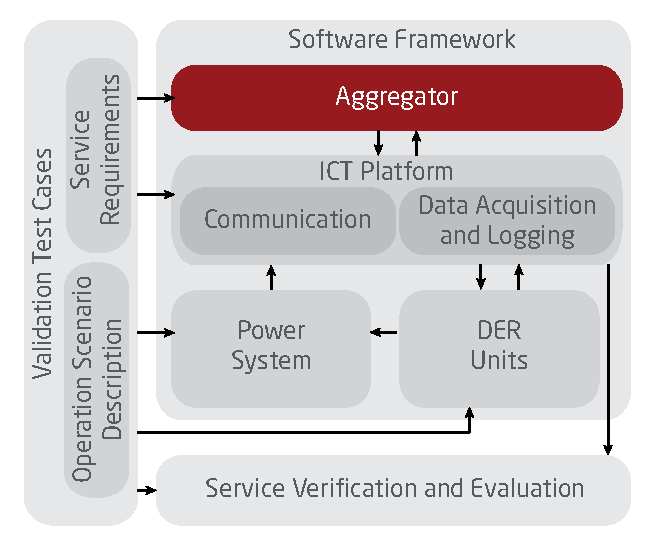
\includegraphics[width=0.5\textwidth]{framework/framework.eps}\label{fig:frameworkbig}
\end{figure}
\marginnote{A recording of the iPower demonstration can be found at \cite{ipowerdemo}.}
\section{Procedure for Validation of Aggregators} 
\newsection{F}{rom the previous} section it is clear that the service requirements form an essential part of the aggregator validation process. Service requirements are discussed in the depth in Chapter~\ref{cha:services}, but a set of test service requirement metrics have been formulated as part of the test method and are presented here.

A set of performance metrics must defined to measure how disturbances\footnote{See Figure~\ref{sec:servreqmet} for a visual representation of how disturbances affect the aggregator} affect service delivery. Based upon the current ancillary service definition, the chosen metrics are:
\begin{description}
	\item[Time responsiveness:] how fast can the service be delivered from the moment the reference or measurement signal changes.
	\item[Grid responsiveness:] how well can the aggregator follow changes in the grid state.
	\item[Response accuracy:] how good is the aggregator at providing the full volume that is requested.
\end{description}

It is the TSO that defines the value of these metrics that signify a passed validation test. Since the tests are stochastic, the metric value should also have a stochastic component, this could for example be \emph{time responsiveness} of service provision of 5 seconds with variance of $\pm$ 1 second. The metrics must be measured by an index and while literature has a wide array of indices for measuring performance, a specific index for aggregators is presented in Chapter~\ref{cha:verification}.

The following steps are proposed for designing the test procedure:
\begin{enumerate}
	\item The aggregator informs of the general composition of its portfolio, as well as the service it wants to be validated for.
	\item The tester identifies the appropriate service requirements for the service to be tested for.
	\item The tester identifies the expected normal operation of the aggregator.
	\item The tester defines the test operation scenarios that the aggregator is expected to perform under. The scenarios must define the statistical properties, \eg mean and variance, for the stochastic disturbances affecting the aggregator performance.
	\item The tests are carried out on the aggregator:
		\begin{itemize}
			\item simulation tests must be carried out, going through the appropriate factorial levels defined in the normal operation of the aggregator;
			\item the simulation tests must be replicated with sufficient samples to capture how the error of the inputs propagates through the aggregator;
		\end{itemize}
	\item The aggregator performance is evaluated.	
\end{enumerate}

%Note that the entity performing the validation tests can be an independent party, \eg a third party certifier for aggregators, or it can be the TSO.
Depending on the excitation signals the aggregator is subject to, the tests are divided into two categories:
\begin{itemize}
	\item step/ramp response, and
	\item continuous reference tracking.
\end{itemize}
The kind of test used for the validation will depend on the test scenario description.

In order to ensure that the simulations are correct, a limited selection of cases must be validated with field tests. This also ensures that the communication system between the aggregator and the system operator functions correctly.

To summarize, the validation procedure consists of a series of simulated tests, where the same excitation signal (be it a step/ramp response or a continuous signal) is replicated with enough samples, over a combination of factor levels, to identify the capabilities of the aggregator. A subsample of these tests must be validated through a field test.

An example of how the procedure is applied to an aggregator (without the final field test validation) can be found in Appendix~\ref{app:pscc2016}, Section~\ref{sec:casestudy}.

\section{On Prequalification and Certification of Aggregators}\label{sec:aggpreq}
\newsection{I}{t was previously mentioned} that traditional generator prequalification consists of two steps, the documentation of the generator and the response test. The prequalification process must be adapted to aggregators. Parting from the concepts presented in this chapter, such a prequalification process could be the following:
\begin{enumerate}
	\item \emph{Documentation:} Description of the aggregator capabilities through the functional reference framework\footnote{See Chapter~\ref{cha:aggregator}.}. This can be used as check list for the basic required functionality.
	\item \emph{Validation test:} A set of response tests should be performed, along with the simulation aided validation procedure, in part to validate the aggregator reliability, but also to verify the communication between the TSO control center and the aggregator.
	\item \emph{Monitoring:} Furthermore, aggregator performance should be continually evaluated, and new validation tests should be carried out routinely. This is due to the dynamic nature of the aggregator portfolio, which may regularly change in size and composition, and due to the changes and updates that may come to the control algorithm.
\end{enumerate}

The same process can be applied to a certification process, \ie a process where a third part certifies the aggregator for participation in the different markets. In this case, the aggregator must be validated against other flexibility services, \ie BRP portfolio balancing or distribution system services.

\section{Conclusions Regarding the Validation Framework}
\newsection{T}{he concept of validation} of aggregators is important for the participation of aggregators in both ancillary services markets and other service markets. The original contribution of this work is the application of statistical method for validation test of aggregators. Also, the validation framework was presented, in which it is clear what are the elements that form part of aggregator validation.

In comparison with the traditional test method, the proposed validation procedure must capture the capabilities of a much more complex system, and therefore relies in part on simulations. A weakness in the proposed method is that the validation tests are highly dependable on the accuracy of the used models in the simulation. A way to mitigate this is to make the framework modular so that the tests can be run with hardware-in-the-loop (for model validation of individual units) or so that the framework can be connected to validated models, \eg a Real-Time Digital Simulator (RTDS). The error between the used models and reality must be quantified\fcite{steinbrink2015challenges} and taken into account for the final aggregator certification. Each block in the simulation must use validated models or software. This applies to the communication systems, the grid models and the DER models. The test architecture which validates the aggregators must also be validated.

Future work will consist of further refining the validation architecture, specifically defining the interfaces between modules, and implementing the software platform. Further exploration of the field of \emph{Design of Experiments} may yield better methods than the fractional factorial method for quantifying the capabilities of the aggregator. Also, a set of realistic operation scenarios must be defined.

%!TEX root = ../Thesis.tex
\chapter{Service Modeling and Requirements} % (fold)
\label{cha:services}
\begin{marginfigure}
	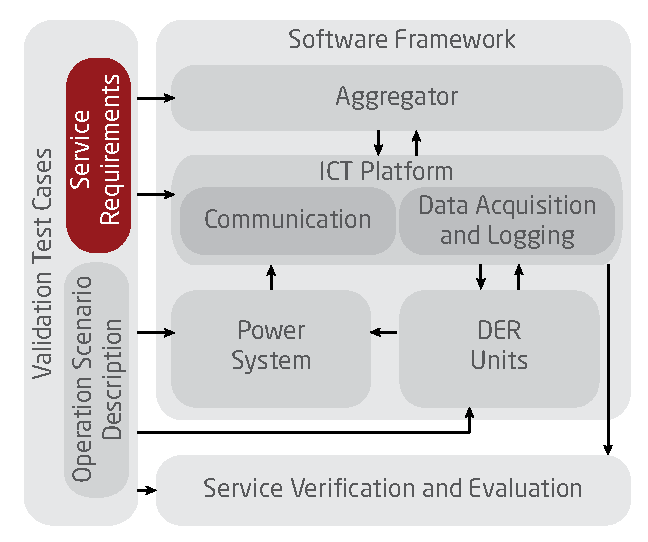
\includegraphics[width=\textwidth]{framework_services.eps}
	\caption{This chapter focuses on the \emph{service definition} block of the aggregator validation framework presented in Chapter~\ref{cha:validation}.}
      \label{fig:framework_services}
\end{marginfigure}

\newchapter{T}{he requirements for ancillary} services are in many countries defined, due to historical reasons, on the assumption that only generators provide ancillary services. It is clear that current service requirements are directly, or indirectly, blocking the integration of aggregators providing DR\fcite{cappers2013assessment,coalition2014mapping}. If aggregators are to be successfully integrated into the power system, the rules and requirements for participation must be changed. This chapter presents two contributions to integrating aggregators in the power system: a modeling method for service requirements, and a proposal for the restructuring of requirements for ancillary services. A method for modeling service requirements is important because the resulting models form the benchmark for the performance evaluation and verification of the aggregator (see Chapter~\ref{cha:verification}), as well as being a direct input to the aggregator (see Chapter~\ref{cha:aggregator}). The redefinition of ancillary service requirements is important since it will remove the barriers for aggregator participation in the AS markets, allowing system operators to utilize the properties of all available resources, both traditional and new, in an optimal way. 

The concepts presented in this section are part of a submitted journal paper\fcite{bondy2016method} which can be found in Appendix~\ref{app:tsg} and a draft journal paper\fcite{bondy2016redefining} found in Appendix~\ref{app:ddras}, as well as work done as a collaborating author for a conference paper\fcite{heussen2013a} and a technical report written for the iPower consortium\fcite{bondy2014powermax}. Section~\ref{sec:backgroundservicesandreq} discusses different kinds of services that aggregators can provide and Section~\ref{sec:modelingAS} presents how these can be modeled. These models are directly related to the \emph{service requirements} block in the aggregator validation framework (see Figure~\ref{fig:framework_services}). In Section~\ref{sec:RedefiningAncillaryServiceRequirements} a proposal for how ancillary service requirements can be reformulated in order to be technology agnostic. 

%Content of this chapter is the work done at LBNL and through the iPower demo.
%\begin{itemize}
%	\item Service definition
%	\item What are aggregators expected to deliver?
%	\item PowerMax service requirements
%	\item Redefining Ancillary Services Requirements for Technology Agnostic Resources
%\end{itemize}

\section{Background}\label{sec:backgroundservicesandreq} % (fold)
\newsection{T}{he following section outlines} concepts related to the definition and requirements of services at TSO and DSO level. While services for the TSO (ancillary services) are well established, DSO and BRP services are a relatively new concepts which are being discussed, \eg in the iPower project\fcite{ipower2013development}. Also, the concept of Service Oriented Architectures is presented.
\subsection{What are Ancillary Services?} % (fold)
\label{sub:ancillaryservicesdef}
Defining what \gls{as} are, as well as which services the term includes, is difficult. This is due to both the differences in the way power systems are managed around the world and the differences in the terminology used to refer to such services. There is overlap between the European and US definition\fcite{eurelectric2004,ferc1997} of AS in that both describe them as services used to ensure the reliability of the power system. In both European and US context reliability is addressed by considering \emph{system adequacy} and \emph{security} \footnote{NERC also used the term system security, but in September 2001 security became synonymous with homeland protection in the US. Now it uses the term \emph{operating reliability} \cite{nerc2007definition}}. \emph{System adequacy} is the power system's ability to supply the electricity demand at all times and \emph{security} is the ability to withstand sudden disturbances.

Generally, maintaining an adequate and secure power system means maintaining the power system operating at nominal frequency and voltage. In cases where the power system deviates from nominal operation, either due to natural fluctuations in production/consumption or faults in the system, the system operators will activate ancillary services to restore normal operation. 

Some countries, \eg Denmark, consider voltage control, black start capabilities, short circuit control and reactive reserves as AS. This work focuses on those services that use active power to maintain the nominal frequency of the grid. In Europe\footnote{ENTSO-E changed in 2013 its nomenclature of AS, and the three presented here correspond roughly to the classical primary, secondary and tertiary reserves as presented in \cite{Rebours}.} these services are \glspl{fcr}, \glspl{frr} (either automatic\footnote{In the United States, regulation is used for system balancing. This service corresponds to automatic FRR.} or manual), and \glspl{rr}\fcite{entsoe2013network}.

These reserves are activated as illustrated in Figure~\ref{fig:MAINfreqcont}. The FCR is the fastest reserve and reacts automatically upon the grid measurements. Its role is to stop frequency excursions and its effectiveness can be measured by the \emph{frequency nadir} \cite{eto2010use}. The FRR is activated by tracking the \gls{agc} signal, or through manual activation by the system operator, relieves the FCR (allowing the FCR to be available again) and restores the frequency to the nominal value. The RR relieve the FRR, usually through rescheduling of units or by bringing inactive units online.

\begin{figure}[htbp!]
\centering
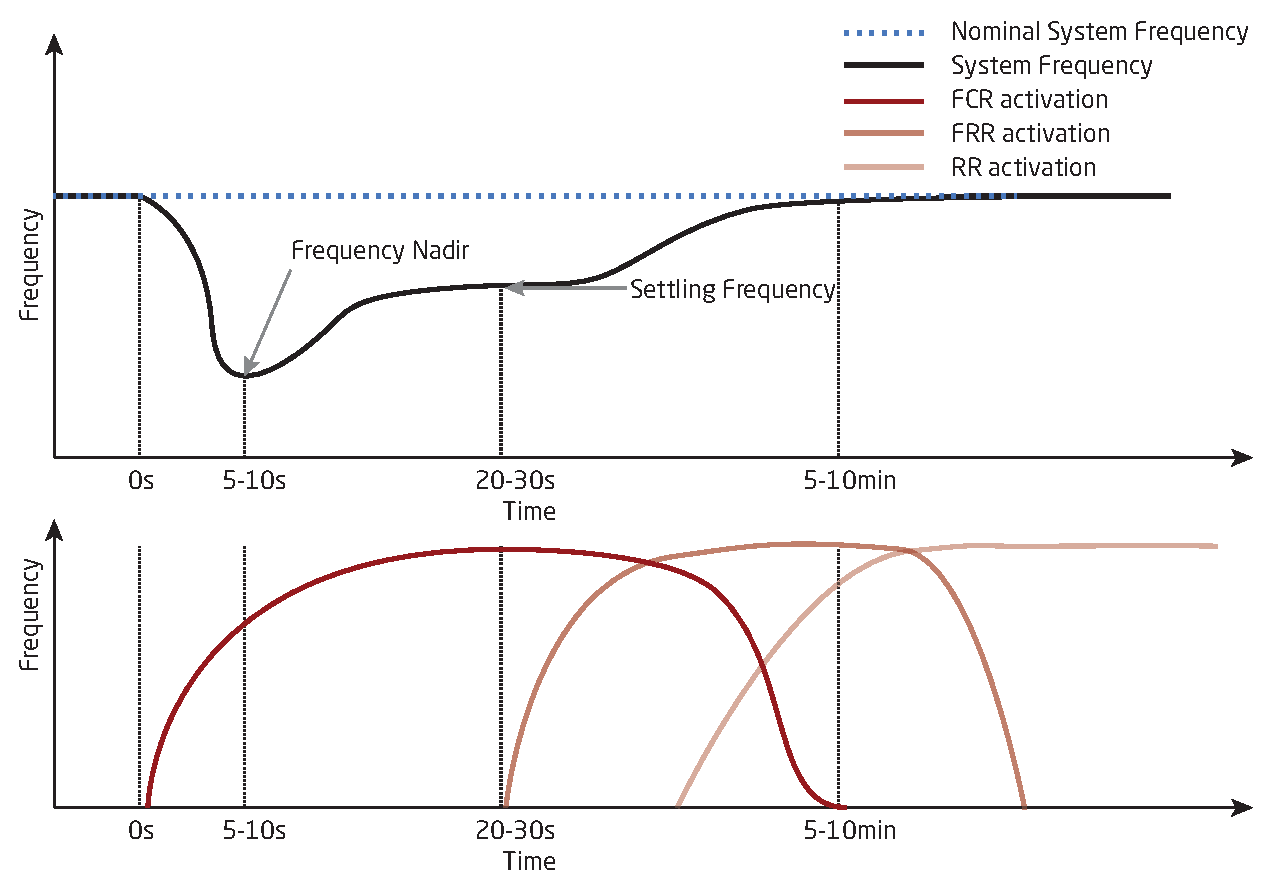
\includegraphics[width=0.9\textwidth]{frequency_contingency.eps}
\caption{The ancillary services are activated sequentially after a frequency contingency. In systems with high inertia the frequency nadir will occur at frequencies closer to the nominal frequency.}
\label{fig:MAINfreqcont}
\end{figure}

% subsection What are Ancillary Services? (end)
\subsection{Requirements for Ancillary Services} % (fold)
\label{sub:servreqAS}
Because AS are essential for the secure operation of the system, the system operators have requirements and restrictions on the units providing AS. A super-set of requirements across different systems was presented by \emph{Rebours}\fcite{Rebours}, and following his overview we classify requirements into three categories:
\begin{description}
	\item[temporal requirements] which relate to how fast and for how long a service must be delivered;
	\item[resource tuning requirements] which relate to specific values that tuning parameters in the resource must have;
	\item[market requirements] which relate to bid sizes and similar parameters in systems where services are acquired through market mechanisms.
\end{description}

Of these three categories, only the temporal requirements relate to service performance. Furthermore, in most systems, the requirements are implicitly defined for traditional generation units. This means that most service requirements are oriented towards the least common denominator of service providers, e.g. a unit providing FCR should provide half of the service within 15 seconds and full response within 30 seconds\fcite{EnerginetAncillary}. A variety of generation and consumption units would be able to provide this service faster, but this quality is not rewarded. Another example is the requirement of having a PI-controller on units providing FRR in order to track the AGC signal. Such a controller is infeasible on distributed systems, but other modern controllers can provide offset-free control with similar properties. This means that the historical requirements for units participating in AS markets in many countries act implicitly, or explicitly, as barriers for new technologies to enter the market\fcite{cappers2013assessment,coalition2014mapping}.%\todo{should I put in a more thorough description of FCR, FRR and RR, like what we have in the DDRAS paper?}

The concept of using demand side management to help the secure operation of the power grid has existed in different forms since the late 1970s\fcite{lampropoulos2013history}. But in recent years, the introduction of new consumption and generation technologies, \ie DERs, along with the roll-out of a smart metering infrastructure and the advances in ICT, has lead to the new opportunities in using smart control of small scale consumption/production as a service to the power grid. There is a large body of literature\fcite{oconnell2014benefits} concerning DR, and proposals to use it for AS\fcite{vrettos2015integrating,mathieu2012using,zarogiannis2014dynamic}.%\clearpage
% subsection Service Requirements for Ancillary Services (end)
\subsection{Distribution System Services} % (fold)
\label{sub:dsoservices}
As the amount of DERs installed at distribution level increases, the DSOs face new operational problems. Mainly, the increase in electric load will cause congestion and voltage issues. The traditional way of handling these are through reinforcement of the grid assets. Given the high cost of installing new cables, and the uncertainty in how the electricity consumption will change in the future, the use of flexibility services will be an attractive alternative.

One of the main outcomes of the iPower project was the definition of a set of flexibility services that demand aggregators can provide DSOs\fcite{ipower2013development} for congestion management or voltage issues. The requirements for three of the congestion management services have been further detailed individually\footnote{The services requirements were detailed in the following technical reports\cite{hansen2013flech,biegel2014flech,bondy2014powermax}.}, and aggregator architectures have been designed to provide both congestion management\fcite{hu2014coordinated} and voltage support\fcite{han2014assessment}. At the same time, the concept of the \gls{flech} has been designed as a platform to enable the transparent contracting of flexibility\fcite{heussen2013a}.

An example of a flexibility service is the \emph{PowerMax}\fcite{bondy2014powermax} service, where the aggregator maintains the total consumption of its portfolio under a limit, within a specified period of time. This means that the aggregator is free to manipulate its portfolio as long as its peak load is below the limit specified by the DSO.
% subsection DSO Services (end)
\subsection{BRP Portfolio Balance Service} % (fold)
\label{sub:BRPPortfolioBalance}
The idea of using aggregators for internal balancing of BRPs was also explored in the iPower project\fcite{tougaard2015flech}. The main objective of such a service is for the aggregator to provide services to BRPs so that they can avoid imbalance costs. This service is similar to FRR, except the contract is with a BRP, which means that contracted volumes will usually be smaller, and the acquisition horizon shorter. BRP portfolio balance services must be acquired 1 hour to 5 minutes before the activation period, and must be cheaper than the imbalance cost.

The concept of BRP services is also analysed by the Universal Smart Energy Framework (USEF) foundation. They propose four different BRP services\fcite{usef2015}:
\begin{itemize}
	\item Day-ahead portfolio optimization,
	\item Intraday portfolio optimization,
	\item Self-balancing,
	\item Generation optimization.
\end{itemize}

% subsection BRP Portfolio Balance (end)
\subsection{Asset Management Services} % (fold)
\label{sub:assetmanagementservices}
In Chapter~\ref{cha:aggregator} the concept of \gls{ams} is introduced as the services that an aggregator provides to the owner of the DERs, or flexibility assets. An example of this is the case where the aggregator is an EV fleet operator that has the contractual responsibility of maintaining all EVs in the fleet within a certain \gls{soc}. The purpose of validating aggregators for these services is that flexibility asset owners can use the validation as a trust measure.

The main idea behind AMS is that the flexibility assets have a primary purpose, which is to satisfy the needs of their owner. The aggregator can use the flexibility of the units as long as the primary purpose is respected. Thus, from the perspective of customer comfort, an aggregator that is better at AMS is more desirable. 
% subsection Asset Management Servc (end)

\subsection{Service Oriented Architectures} % (fold)
\label{sub:ServiceOrientedArchitectures}
The concept of \gls{soa} comes from the field of computer science and is an approach to creating software architectures based upon the concept of services. Parallels to this approach can be drawn with the way ancillary service provision works in unbundled energy markets. 

Under the SOA paradigm, service is defined as: a logical representation of a repeatable business activity that has a specified outcome, is self-contained, may be composed of other services and is a \emph{black box} to consumers of the service\fcite{opengroupsoa}. The following concepts are central to the SOAs:
\begin{description}
	\item[Standardized service contracts:] These can be interpreted as interfaces, in that they describe the service purpose and functionality\fcite{Erl08thesoa}.
	\item[\gls{sla}:] These are part of the standardized service contracts which define the service performance metrics with corresponding Service Level Objectives. SLAs can be interpreted as the requirements defined in an ancillary service contract.
	\item[\gls{slo}:] These define the agreed means for measuring performance.
\end{description}
% subsection Service Oriented Architectures (end)
% section Background on Aggregator Services (end)
\section{Modeling of Service Requirements} % (fold)
\label{sec:modelingAS}
\newsection{T}{he validation framework} presented in Chapter~\ref{cha:validation} uses the \emph{service requirements} as a benchmark towards which the aggregator is evaluated. This is because the requirements contain the control objective of the aggregator. Currently, requirements for services are encoded within the contractual agreements between system operator and service provider. A standard method is needed for extracting this information and building a model that can be used for benchmarking, \ie a \emph{standardized service contracts} must be defined with their corresponding SLA and SLO.

By analysing the services presented in Section~\ref{sec:backgroundservicesandreq}, the following requirements for the service requirements model are defined:
\begin{description}
    \item[M-R1] the model must clearly identify the SLOs of the service,
    \item[M-R2] the model must incorporate both the ideal and acceptable service provision in a measurable/quantifiable way, \ie performance metrics must be able to be applied to it,
    \item[M-R3] the models must be technology agnostic,
    \item[M-R4] since flexibility services imply a change of consumption pattern over a period of time, the models must consist of time series.
\end{description}

Based upon these requirements, a method for translating the contracts into a time series model has been developed. The method consists of the following six steps:
%form have been identified as a generic method for modeling ancillary services. The steps are exemplified by DSO services defined in  and TSO services defined in :
\begin{enumerate}
	\item Identify physical parameters defining the service [M-R1].
  \begin{itemize}
    \item \eg Power production or consumption, measured grid frequency, time measurements, etc.% Including maximum measuring sensitivities.
  \end{itemize}
  \item Identify the dynamic behaviors of the service related to system parameters (if any) [M-R1].
  \begin{itemize}
    \item \eg FCR expects a linear relation between a deviation from the nominal grid frequency and the generator set-point.% Power-cap has a dynamic relationship between feeder load and the controllable load power in order to keep the total feeder load at a $P_{DSO,Ref}$ value.
    %\item PowerMax is not dynamic. The aggregator must control $\Delta P_{Agg}$ to ensure that he does not violate $P_{max,Agg}$. But the service does not require a dynamic behavior related to a system parameter like primary frequency regulation and PowerCap.
  \end{itemize}
  \item Identify the physical size of the service and the tolerated error [M-R2]. % Both ideal service and minimum required service.
  \begin{itemize}
    \item \eg the volume of the bid for FCR. %Physical size is for example $P_{max,Agg}$ for PowerMax service or
%    \item Tolerance is for example $P_{max,Agg}+P_{tolerance}$ for the PowerMax service and allowed dead-band for DK1 primary reserve.
  \end{itemize}
  \item Identify the ideal response time of the service and acceptable response [M-R2].
  \begin{itemize}
%    \item Most contracts comes with some timing specifying how fast the service provider must act.
    \item \eg FCR in western Denmark must be 50 \% of activated within 15 s and 100 \% within 30 s.
%    \item The ideal service is for example an instantaneous step in power to 100 \% of set-point for DK1 primary reserve.
  \end{itemize}
  \item Based on the dynamics, size and timing of the service, as well as the tolerated errors from points 1--4, develop a time series for ideal and acceptable service provision. The model will be a set of time series: $\mathbf{x}_{ideal}(t)$ for ideal response and $\mathbf{x}_{acc}(t)$ for acceptable response. Both time series can be a scalar or a vector, e.g. $\mathbf{x}_{acc}(t)$ can be formed by a set of upper and lower tolerance bounds or simply by an upper bound [M-R4].
  \item Identify how the service error is to be measured [M-R1].
\end{enumerate}
By only defining the SLA models in terms of performance, not in specific unit capabilities, the models implicitly comply with [M-R3].

Furthermore, the analysed services can be divided into three patterns:
\begin{description}
	\item[Reference Tracking:] Services where a reference signal must be followed, \eg regulation in the United States.
	\item[Band Service:] Services where the output is able vary between an upper and lower limit, \eg smart charging of a fleet of EVs.
	\item[Cap Service:] Services where the output must respect either a upper or lower bound, \eg the \emph{PowerMax} service.
\end{description}

Based upon the three kinds of service, the service error, \ie step \emph{6} in the modeling method, can be measured the following ways:
\subsection*{Reference tracking}

Reference tracking error can be calculated as:
\begin{equation}\label{MAINeq:ref_error}
e(t) = x_{meas}(t) - x_{ideal}(t),
\end{equation}
\begin{marginfigure}
	\includegraphics[width=\textwidth]{tracking_error2.eps}
	\caption{Error in reference tracking.}
      \label{fig:reftrackerrorMAIN}
\end{marginfigure}
where $x_{meas}(t)$ is the measured output, \eg the total load of the aggregator portfolio, and $x_{ideal}(t)$ is the ideal response defined in the service model. This definition will lead $e<0$ for measured values below the ideal and $e>0$ for values above the ideal. In this case $\mathbf{x}_{acc}(t)$ will be a band around $x_{ideal}(t)$, and the values of $\mathbf{x}_{acc}(t)$ do not need to be symmetric.

\subsection*{Band service}
The ideal response in a band service is defined as $ \mathbf{x}_{ideal}(t)= [x_{min}(t),x_{max}(t)]$. The error in the band service can therefore be estimated by:
\begin{equation}\label{MAINeq:band_error}
e(t)=
\begin{cases}
x_{meas}(t) - x_{min}(t) , & x_{meas}(t) < x_{min}(t)  \\
0, & x_{min}(t) \leq x_{meas}(t) \leq x_{max}(t) \\
x_{meas}(t) - x_{max}(t), & x_{meas}(t)  > x_{max}(t).  
\end{cases}
\end{equation}
\begin{marginfigure}
	\includegraphics[width=\textwidth]{band_error2.eps}
	\caption{Error in band service.}
      \label{fig:banderrorMAIN}
\end{marginfigure}

In this case, the $\mathbf{x}_{acc}(t)$ is a set of values that surrounds the band defined by $ \mathbf{x}_{ideal}(t)$, as seen in Fig.~\ref{fig:RefErr}. The values of $\mathbf{x}_{acc}(t)$ do not need to be symmetric around the band.

\subsection*{Cap service}
%Maximum/minimum cap error only counts the error when performance is above/below some ideal value. 
In cap services, error is only tracked when $x_{meas}(t)$ is either above or below a given a limit value.
Maximum cap error is calculated as shown in \eqref{MAINeq:maxmin_cap} and minimum cap can be similarly calculated. In \eqref{MAINeq:maxmin_cap}, $x_{max}(t)$ is the ideal maximum limit according to the service contract:

\begin{equation}\label{MAINeq:maxmin_cap}
e(t)=
\begin{cases}
x_{meas}(t)-x_{max}(t), & x_{meas}(t) > x_{max}(t) \\
0, & x_{meas}(t) \leq x_{max}(t).
\end{cases}
\end{equation}
\begin{marginfigure}
	\includegraphics[width=\textwidth]{cap_error2.eps}
	\caption{Error in cap service.}
      \label{fig:caperrorMAIN}
\end{marginfigure}

In the cap service, $x_{acc}(t)$ is a limit that either lies below $x_{min}(t)$ or above $x_{max}(t)$.

The applicability of these models is showcased in Section~\ref{sec:MAINQoS}.
% section Modeling of Ancillary Services (end)

%
\section{Restructuring Ancillary Service Requirements} % (fold)
\label{sec:RedefiningAncillaryServiceRequirements}
\marginnote{This section is a summary of the draft paper in Appendix~\ref{app:ddras}. Some of the concepts missing in the draft paper have been introduced here.}
Until now, system operators have been able to arrest frequency excursions fast enough because of the inherent system inertia. With the increasing penetration of wind power in the system, the electricity prices are lowered and operating fossil-fueled generator becomes economically unfeasible. This has the effect of reducing the system inertia, and reducing the availability of AS resources. Therefore new AS sources with faster response times are required. \emph{Vrettos et al.}\fcite{vrettos2015integrating} show that if FCR is provided by DR (with a very fast response), the frequency nadir occurs at higher frequencies.
Also, \emph{Makarov et al.}\fcite[][16\baselineskip]{makarov2008assessing} argue that the value of regulation resources can be defined based upon the ramp capabilities of the service providing units. Faster reacting units are more valuable to system operators, since they help arrest the frequency excursion faster and at a higher nadir.% It does require changes to the AGC in order to utilize the fast response, but this would also lead to the need for fewer reserves.

AS requirements are specified by a system operator based on the desired control response for a particular power system, under the implicit assumption that the ideal unit response corresponds to a scalar fraction of the required system response. Today, these requirements --- as reflected in the service definition --- are not differentiated according to the capabilities of the unit providing the service. Therefore, service definitions are designed to accommodate the least capable unit in the portfolio. As a consequence, more capable units are not being fully utilized, leading to excess contracting of service providers.

 In this section a new form of defining AS requirements is presented, which has as an objective to allow all units to participate in the AS markets on equal footing. The main assumption is that all units can be valuable for AS provision, even when they do not fully comply with current requirements, and that the system operators will be able to manage the system better if the capabilities of all available resources are utilized. Also, units should be remunerated based upon the value they represent to the operation of the system, and their performance compared to these expected values.

Regulative authorities have concluded that fast reacting units are valuable for the system operation, and started programs to benefit of these resources. An example of this is FERC order 755 (Pay for Performance) which has led to PJM splitting their regulation market product into RegA, for slow reacting units, and RegD for fast reacting units. The product differentiation approach has been a success for PJM, but  splitting the market may still lead to suboptimal utilization of units and does not address the issue of new technologies being effectively excluded from certain markets.  We propose instead to restructure the ancillary service definitions such that all types of service providers participate with the same market product defined by a set of optimal performance parameters, and not by minimum requirements. This means that the all entities providing a given ancillary service are optimally cleared under a single market.

\subsection{The Overall Approach} % (fold)
\label{sub:TheOverallApproach}
The restructuring of AS requirements is formed by the following key concepts:
\begin{enumerate}
	\item The system operator is able to formulate an overall \emph{ideal AS response} that can be achieved through an optimal mix of resources. Any resource can make a bid for providing part of this ideal response.
	\item The \emph{parametrization of AS bid}, where the parameter values of each unit/bid reflect the service provider's capabilities to partially fulfill the ideal response. This avoids excluding units that may have useful capabilities in one parameter, e.g. very fast ramp rate, but low capabilities in another parameters, e.g. only holding the response for a short time. Such a service definition allows compliance to be measured on a linear rather than a binary scale: In addition to compliance and noncompliance, different levels of partial compliance are possible.
	\item Clearing all units under a \emph{generalized single clearing-price auction} allows constructing an optimal portfolio, and enables competition between all resources, leading to lower prices.
    \item \emph{Performance-based remuneration} gives incentive to better AS provision and enables transparent performance-based clearing of the market.
\end{enumerate}

These points are further described in the following subsections, although the focus of this work is on the \emph{parametrization of AS bid} and the proposal for a market clearing mechanism. The concepts are explained in the rest of this section and Section~\ref{sub:ApproachExample} presents an example of the approach.
% subsection The Overall Approach (end)
\subsection*{Ideal Service Tender} % (fold)
\label{sub:IdealServiceTender}
\emph{Makarov et al.}\fcite{makarov2008assessing} define the ideal source for AS as one with ``unlimited capabilities in terms of response time, energy output, ability to frequently reverse their output, ability to respond and follow the AGC setpoint changes, and size.''\footnote{For this kind of response to be optimal, changes must be made to the AGC algorithm \cite{peydayesh2012effects}.} It is impossible for any one unit to possess these characteristics, but system operators aim at achieving this kind of system response by contracting several units.

In order to define an ideal tender the system operator must identify the needs of the system through metrics as those presented in Section~\ref{subsec:perfindicesinpowsys}, \eg the \emph{nadir-based frequency response} proposed by \emph{Eto et al.}\fcite{eto2010use}. By understanding the specific needs the system, the system operator will be able to define which are the relevant parameters that will satisfy these needs.
% subsection Ideal Service Tender (end)
\subsection*{Service Parametrization} % (fold)
\label{sub:ServiceParametrization}
The overall ideal service requirements can be expressed as:
\begin{equation}
	S^* = f_m(\textbf{x}^*) \label{eq:optimaltender}
\end{equation}
where $\textbf{x}^*$ is a vector of ideal parameter values and $f_m(\cdot)$ a function that translates the parameters $\textbf{x}$ into a model, e.g. into a time series as shown in Section~\ref{sec:modelingAS}. Furthermore, the system operator must inform how the parameters are valued with respect to the $S^*$, which is done through a capability value:
\begin{align}
    \kappa &= g(\mathbf{x}) \\
    \kappa &\in [0,1].
\end{align}

% subsection Service Parametrization (end)

\subsection*{Market Mechanism} % (fold)
\label{sub:MarketMechanism}
It is impossible to restructure the AS definition without addressing the market mechanism for determining the optimal set of resources. The market should be designed as a single clearing price auction, in which each resource bid is adjusted by \emph{two} factors for bid quality: 1) the capability value $\kappa$ and 2) a historical performance\footnote{The historical performance parameter can also be interpreted as an availability parameter, or certainty parameter. PJM also uses the historical performance score of unit for the settlement.} parameter $\eta^{hist}$. The historical performance parameter determines how close the unit has followed the properties defined in $\kappa$. 
% subsection Market Mechanism (end)

\subsection*{Performance Based Remuneration} % (fold)
\label{sub:PerformanceBasedRemuneration}
The estimation of the service provision performance can be done in different ways, depending on which parameters the system operator deems to be the most critical. The concept of performance assessment is discussed in Chapter~\ref{cha:verification}, and performance index is introduced there. Here it suffices to say that the performance measurement is a function of the error in service delivery:
\begin{align}
	\eta &= c(e(t)), \label{eq:perfindexsimple}\\
	\eta &\in [0,1]
\end{align}

This value, along with the capability value $\kappa$ should form part of the service remuneration. 
% subsection Performance Based Remuneration (end)
\subsection{Approach Example} % (fold)
\label{sub:ApproachExample}
This section presents an implementation example of the AS requirements restructure. It must be noted that these are only examples and further research should be done in how best to implement the presented concepts.
\subsection*{Ideal Tender}
A system operator could determine that the ideal system response to a frequency excursion is the one that has a resulting frequency nadir at the settling frequency (thus minimizing the risk of tripping the under-frequency relays). Based upon the inertia in its system, the system operator determines the volume ($V_{tot}$) needed as well as the response characteristics needed to achieve this, see Figure~\ref{fig:idealresponse}.

\begin{figure}[htbp!]
\centering
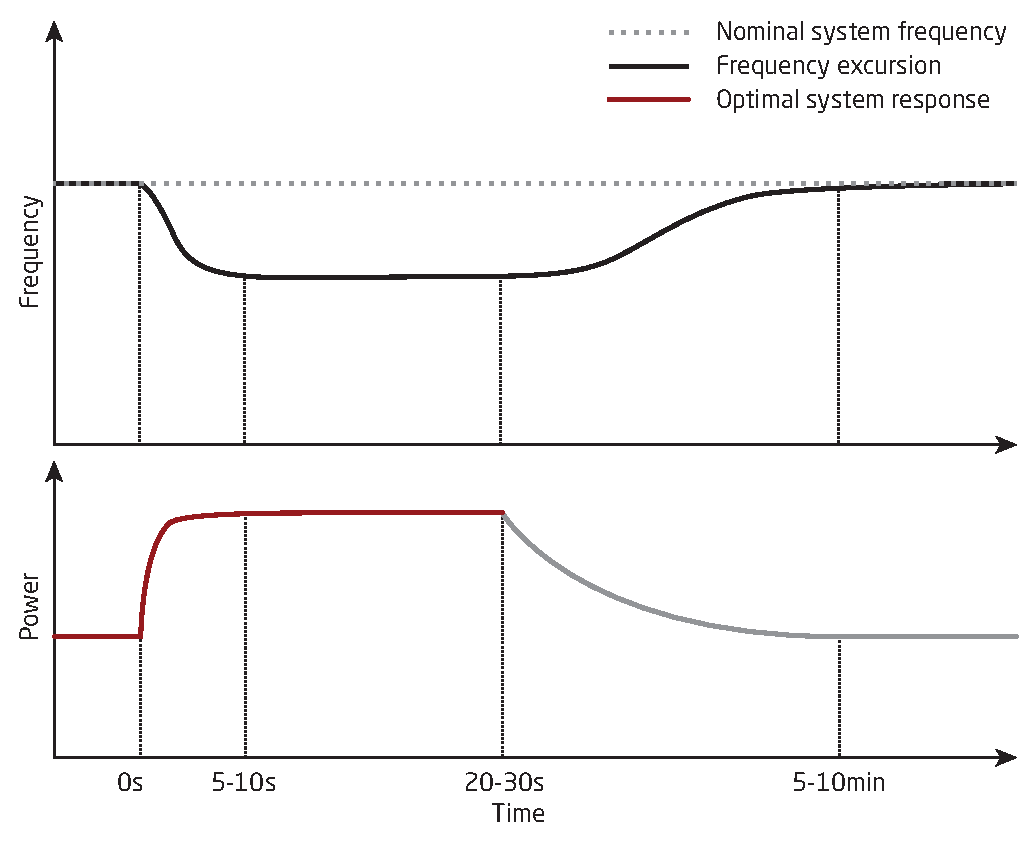
\includegraphics[width=0.9\columnwidth]{primary_frequency_control_ideal.eps}
\caption{In this case, the ramp of the ideal response is mainly determined by the system inertia and is to be sustained until FRR can be activated.}
\label{fig:idealresponse}
\end{figure}

\subsection*{Service Parametrization}
A system operator decides that the FCR in their market is defined by $\textbf{x} = [\tau_r,\tau_d,V]$, where $\tau_r$ is the rise time of the service, $\tau_d$ is the duration of the service, and $V$ is the volume of the service. Due to the properties in its system, it decides that $\textbf{x}^* = [30 s, 20 min, 90 MW]$. The capability value of each bidder is calculated by:
\begin{equation}
	\kappa_i = \alpha_1 \frac{\tau_{r,0}}{\max({\tau_{r,0},\tau_{r,i})}} + \alpha_2  \frac{\min(\tau_{d,0},\tau_{d,i})}{\tau_{d,0}} + \alpha_3 \frac{V_i}{V_{tot}}, \quad \forall \, i \in \Omega \label{eq:kappa_primfreq}
\end{equation}
where $\tau_{r,0}$ and $\tau_{d,0}$ are a nominal value the system operator sets, $\tau_{r,i}$ and $\tau_{d,i}$ are the actual parameter values for each bidder, $\frac{V_i}{V_{tot}}$ is the bid contribution to the total required volume, and $\Omega$ is the pool of bids. Finally, $\sum_{i} \alpha_i = 1$, and in this case could be $\alpha_1,\alpha_2 = \frac{2}{5}, \alpha_3 = \frac{1}{5}$.

\subsection*{Market Mechanism}
The proposed clearing mechanism identifies a common clearing price based on the most expensive accepted bid\footnote{This is similar to the merit order lists used in \eg the Nordic system for Manual Regulating Power\cite{bondy2013}.}:
%Clearing principles
\begin{equation}
    P^\mathtt{clear} = \max P^\mathtt{bid}_i, \quad i \in \Omega^\mathtt{acc}
\end{equation}
where $\Omega^{acc}\subseteq \Omega$ is the subset of accepted bids of the set of received bids $\Omega$. 
The clearing mechanism selects the subset of bids which offer the cheapest overall clearing cost and meet the tender requirements with a given certainty of availability: 
\begin{align}
	\Omega^\mathtt{acc} = &\mathtt{argmin}_{\Omega^\mathtt{hyp} \in \mathcal P(\Omega)} &\sum_{i\in \Omega^\mathtt{hyp}}{\kappa_i P^\mathtt{clear}_{\Omega^{hyp}} }  \\
	  &\text{subject to} &\sum_{i\in \Omega^\mathtt{hyp}} f_m(\mathbf{x_i}) \geq S^*   \\
      &~  &\eta^{hist}_i \geq \eta^{hist}_{min} &\quad \forall \, i \in \Omega^\mathtt{hyp} 
\end{align}
Where $\mathcal P(\Omega)$ denotes the Power Set of $\Omega$ and $\Omega^{hyp}$ is a (hypothesis) subset of the Power Set. $S^*$ is the ideal tender from Eq.~\eqref{eq:optimaltender} and $\eta^{hist}_{min}$ is the minimum historical performance requirement to participate in the market\footnote{This value represents how averse the system operator is to risk, and could also be considered part of the service parameters $\textbf{x}$.}.

\subsection*{Performance Based Remuneration}
We propose that remuneration must be based on the performance evaluation of the service provision:
\begin{equation}
	P^\mathtt{rem}_i = \eta_i\kappa_i  P^\mathtt{clear} \qquad \forall \, i \in \Omega^\mathtt{acc}.\label{eq:MAINperfrem}
\end{equation}
Thus, remuneration is based upon the value the resource has to the grid operator, how well it performs, and the most expensive activated resource.

% subsection Approach Example (end)
% section Redefining Ancillary Service Requirements (end)

\section{Conclusions on Service Requirements} % (fold)
\label{sec:ConclusionsServiceRequirements}
\newsection{A}{ggregators have become} possible sources for ancillary services and distribution system services. While system operators are aware of the potential in using flexibility for system balancing, the ancillary service requirements have not been changed in order to accommodate this new technology. This chapter presented a novel proposal for solving this issue, by restructuring the ancillary service requirements based upon a set of optimal parameters instead of the limiting minimum requirements found in many systems today.

Also, a method for modeling services was shown. The resulting models are relevant for the validation framework in that they provide the benchmark towards which aggregators must perform. In Chapter~\ref{cha:verification} it is shown how the service models can be used for performance assessment and verification of services.

The work presented in this chapter differs from the rest of the thesis, in that the concepts presented here are not focused on the aggregator itself. The service modeling method can be applied to any kind of service, not necessarily those provided to be provided by aggregators, and the objective of the ancillary service restructuring is to include any new technology, not only aggregators providing DR.

The AS restructuring is part of a draft paper and needs to be further refined. The implementation of the presented concepts needs further research, especially the mapping from service needs to parametrization, as well as a fair market mechanism.


% section Conclusions on Service Requirements (end)
% chapter Service Requirements (end)

%!TEX root = ../Thesis.tex
\chapter{Performance Assessment \& Verification of Aggregator Services} % (fold)
\label{cha:verification}
\begin{marginfigure}
	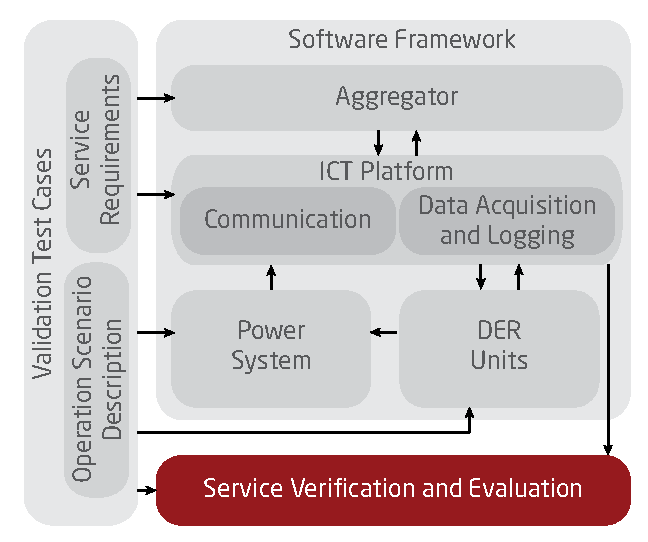
\includegraphics[width=\textwidth]{framework_verification.eps}
	\caption{This chapter focuses on the \emph{service verification and evaluation} block of the aggregator validation framework presented in Chapter~\ref{cha:validation}.}
      \label{fig:frameworkverification}
\end{marginfigure}
\newchapter{P}{erformance assessment is the} process\marginnote{The IEEE defines verification as:``confirmation, through the provision of objective evidence, that specified requirements have been fulfilled.''} of quantifying and verifying the provision of a service according to the contractual specifications of the service. Performance assessment usually occurs at three stages\fcite{coalition2014mapping}
\begin{itemize}
	\item To qualify potential resources against service specifications as part of the validation/prequalification procedure.
	\item To verify service conformance to the service specifications during and after service delivery. 
	\item To calculate the amount of service delivered by the resource as part of financial settlements.
\end{itemize}
%\begin{itemize}
%	\item Why is verification an important part of validation?
%	\item Performance Assessment of Aggregators providing Demand Response
%\end{itemize}
%All resources should be held to the performance specifications established by the product. However – demand side and generation side communication requirements will usually need to be designed separately and made appropriate to each. Technical rules often proscribe the use of metered values to base performance and settlements.[from the SEDC report used in the DRAS paper]

This chapter presents a novel set of performance indices developed for aggregator performance assessment which can be applied at the three stages outlined above. The main focus of the results presented is on aggregator validation and service verification. \todo{finish thought here\ldots something about the importance or the relevance}

The initial work on aggregator performance assessment was presented in a conference paper\fcite{bondy2014performance} and further refined in a submitted journal paper\fcite{bondy2016method}. These paper can be found in Appendix~\ref{app:isgt2014} and Appendix~\ref{app:segan}. 


\section{Background}
\newsection{L}{ittle attention has been} given to the problem of performance assessment of aggregator controllers seen from a service-delivery perspective. As stated in Section~\ref{subsec:aggtest}, performance assessment of aggregators has been mostly ad-hoc analysis specific to a problem the designers are trying to solve, but none have taken a systematic approach to the evaluation of aggregators in terms of established service requirements. In this section we present the concept of control performance assessment and performance indices in power systems, which are topics that serve as background for the rest of the chapter.

\subsection{Control Performance Assessment}
Control Performance Assessment (CPA) is already an established field within control engineering. Most of the applications within the field are found in the process industry\fcite{jelali2006overview}, but since aggregators are a control system, and provide control services, it is natural to translate concepts of CPA to the power system. Usually, CPA methods fall within two types:
\begin{itemize}
	\item benchmarking of controllers towards a theoretic optimum, taking stochasticity of the process into account; and
	\item benchmarking against deterministic properties required of the close-loop system.
\end{itemize}

Usually these indices are normed so that for an index $\eta$:
\begin{equation}
	\eta \in [0,1].
\end{equation}

\subsection{Performance Indices in the Power System}
Currently, the concepts of performance indices and evaluation criteria are used in the power system for the general assessment of how well the System Operator is managing the system. But these evaluation concepts are usually tailored to specific services, \eg CPS1 and CPS2\footnote{An alternative to these two Control Performance Standards is formulated in \cite{gross2001analysis}.} used by NERC\fcite{nerc2011balancing} for evaluating regulation, or the \emph{nadir-based frequency response} metric\fcite{eto2010use} used for evaluating the quality of primary frequency control in an area. Other evaluation criteria have the power interruption to the end customer in focus, \eg System Average Interruption Duration Index (SAIDI) and System Average Interruption Frequency Index (SAIFI)\fcite{LaCommare20061845}. 

As part of the FERC order 755\footnote{The order stipulates that all units providing regulation should get remunerated based upon their performance.}, PJM has introduced a performance score for the remuneration of services in the form of:
\begin{equation}
	\text{Performance Score} = A S_A + B S_D +C S_P
\end{equation}
where $S_A$ is an accuracy score, $S_D$ is a delay score, $S_P$ is a precision score, and $A+B+C =1$ are scalar weights. While this is a detailed performance metric, it is tied to the way regulation is done in PJM.

A measure for the performance of aggregators, that is not directed at a single service and that has service delivery in focus, is the topic of this chapter.

\section{Quality of Service}\label{sec:MAINQoS}
\newsection{T}{he concept of Quality}\marginnote{This section relies heavily on the service modeling concepts presented in Section~\ref{sec:modelingAS}, and it is recommended that the reader familiarizes with that section before reading this section.} of Service (QoS) is closely related to the service models presented in Section~\ref{sec:modelingAS}. One of the elements of a service model is the definition of the service error. QoS is an instantaneous measure of how well the aggregator is delivering a service at any given time instant, and can be defined as the scaling of the error to the limits defined in the service model, \ie:
\begin{equation}
	QoS(t) = e(t)C_s(t),
\end{equation}
where $e(t)$ is the error in service delivery and $C_s(t)$ is a time varying normalization factor. This factor ensures that:
\begin{itemize}
	\item $QoS \geq 0$,
	\item for $QoS \leq 1$ the service is considered delivered within the contractual constraints, and
	\item $QoS = 0$ is a perfect service delivery.
\end{itemize}

The original definition proposed in \cite{bondy2014performance} assumed symmetric constraints around the acceptable provision, but in \cite{bondy2016method} this definition was expanded to account for asymmetry, thus $C_s(t)$ is defined as:
\begin{equation}
C_{s}(t) = 
\begin{cases}
\frac{1}{x_{acc,max}(t) - x_{max}(t)}, & e(t) \geq 0 \\
\frac{1}{x_{acc,min}(t) - x_{min}(t)}, & e(t) < 0.
\end{cases}\label{eq:MAINcst}
\end{equation}
where $x_{acc,max/min}$ and $x_{max/min}$ are part of the service model defined in Section~\ref{sec:modelingAS}. A visual representation of the error models and their corresponding \emph{QoS} definition are shown in Figure~\ref{fig:MAINerrorQoS}

\begin{figure}[htpb!]
\centering
\subfloat[Tracking service error]{\includegraphics[width=0.5\columnwidth]{SEGAN/tracking_error2.eps}%
\label{subfig:errortracking}} \subfloat[Tracking service Quality of Service]{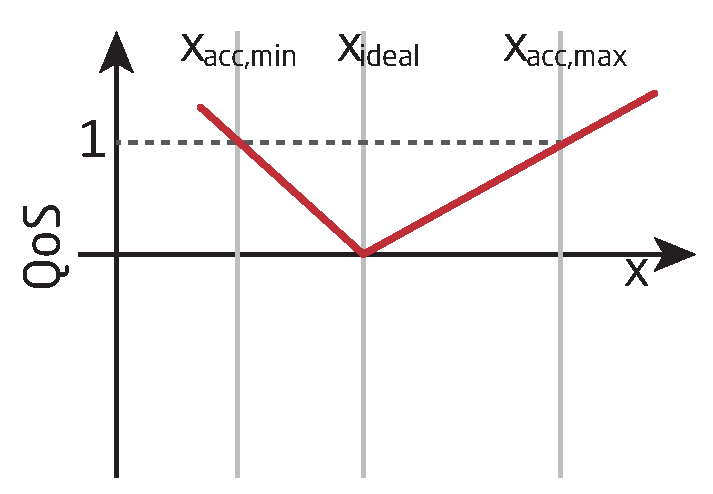
\includegraphics[width=0.5\columnwidth]{SEGAN/tracking_error3.eps}%
\label{subfig:qostracking}}\\
\subfloat[Band service error]{\includegraphics[width=0.5\columnwidth]{SEGAN/band_error2.eps}%
\label{subfig:errorband}}\subfloat[Band service Quality of Service]{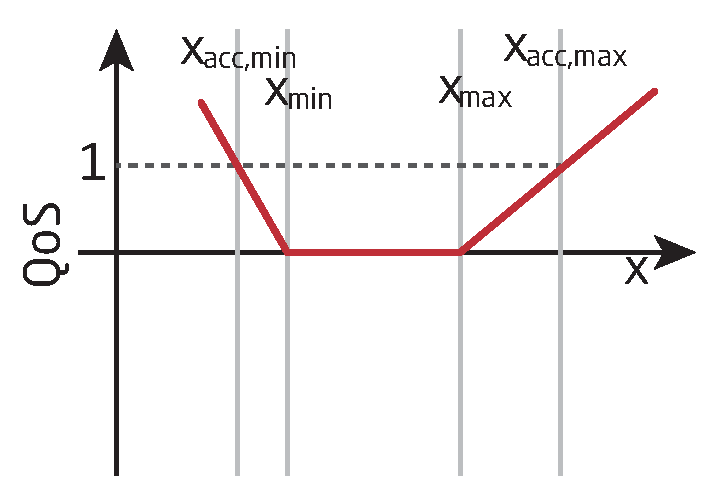
\includegraphics[width=0.5\columnwidth]{SEGAN/band_error3.eps}%
\label{subfig:qosband}}\\
\subfloat[Cap service error]{\includegraphics[width=0.5\columnwidth]{SEGAN/cap_error2.eps}%
\label{subfig:errorcap}}
\subfloat[Cap service Quality of Service]{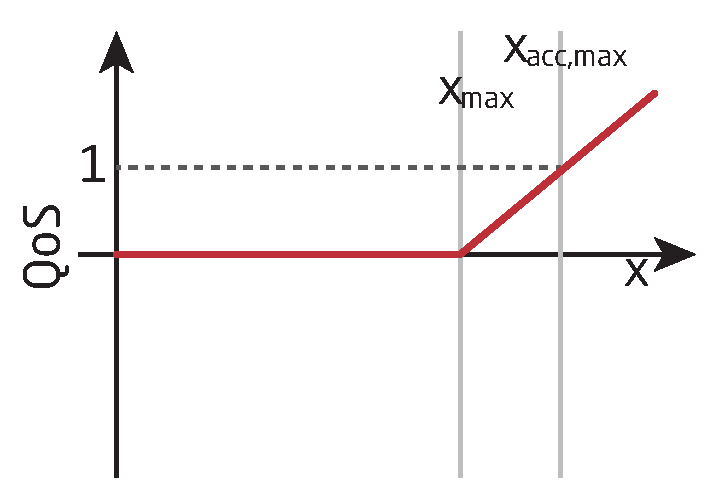
\includegraphics[width=0.5\columnwidth]{SEGAN/cap_error3.eps}%
\label{subfig:qoscap}}
\caption{Error and QoS for the three kinds of services, note that the acceptable band do not need to be symmetric.}
\label{fig:MAINerrorQoS}
\end{figure}

\section{The Aggregator Performance Indices}
\newsection{P}{erformance criteria used for} evaluating controllers usually fall within three categories\fcite{Green}: quality, reliability and energy efficiency. When assessing aggregators, service quality and service reliability define the performance of the aggregator. Four requirements are defined for the performance criteria of aggregators:
\begin{itemize}
	\item[R1] Provide a \emph{quality} measure normalized to the contractual requirements (bounds) of a service. 
	\item[R2] The measure should be normalized with respect to time.
	\item[R3] Provide a \emph{reliability} measure in relation to service non-delivery.
	\item[R4] Each service that the aggregator provides must have a separate, individually verifiable, measure. For example, to evaluate service delivery with respect to ancillary-service delivery, the asset-management quality is irrelevant.
\end{itemize}

To fulfill these requirements two indices are defined:
\begin{itemize}
	\item a service performance assessment index, and
	\item a service verification index.
\end{itemize}

\subsection{Service Performance Assessment index}
The service performance assessment index consists of the weighted average of the normalized root mean square error (RMSE) of the service delivery\footnote{Originally, this index was defined in \cite{bondy2014performance} as the integral square error (ISE) of the service delivery, which was then normalized to a maximum allowable error. This definition does note cope well when the service provision of several services are evaluated at the same time. Therefore, the index was reformulated as the RMSE.}. For evaluation of \emph{K} amount of ancillary services, over discrete time horizon of service delivery \emph{N}, the index is defined:
\begin{align}\label{eq:MAINetaAS}
\eta^{AS} &= \sum^{K}_{i=1} W^{AS}_i \sqrt{\frac{\sum^{N_i}_{t=0} \left( {QoS^{AS}_{i,t}}^{2} \right)}{N_i}}\\
\sum_{i=1}^K W^{AS}_i &= 1 \label{eq:was}
\end{align}
where $QoS^{AS}_{i,t}$ is the truncated $QoS \in [0,1]$ of the ancillary serviced delivery. This definition means that $\eta^{AS} \in [0,1]$, where values close to 0 mean a good service delivery, and values close to 1 mean a bad service delivery. It is expected that in most cases $K=1$, but this definition allows for more services being evaluated at the same time.

The index can be similarly defined for \emph{M} amount of asset management services:
\begin{align}\label{eq:MAINetaAMS}
\eta^{AMS} &= \sum^{M}_{i=1} W^{AMS}_i \sqrt{\frac{\sum^{N_i}_{t=0} \left( {QoS^{AMS}_{i,t}}^{2} \right)}{N_i}}\\
\sum_{i=1}^M W^{AMS}_i &= 1 \label{eq:wams}
\end{align}
It is likely that $M > 1$, \eg if the aggregator is an EV fleet operator for a single large customer. Finally, if an aggregator desires to evaluate its own overall performance, \eg as part of an internal reviewing process, it can combine both kinds of service provision in a weighted average:
\begin{equation}
\eta_{tot} = \alpha \eta^{AS} + (1-\alpha) \eta^{AMS}, \quad \alpha \in [0,1]
\end{equation}
where $\alpha$ is the weight ratio  between the two kinds of service. 

An example of how the service delivery could look for five different aggregators providing the same ancillary service, in this case a reference tracking service, with varying \emph{QoS} is presented in Figure~\ref{fig:indextest3} and the corresponding performance evaluations are presented in Table~\ref{tab:qostest3}. This scenario shows a wide spread of \emph{QoS}, which is reflected in the $\eta$ values. The first aggregator has a relatively good performance and therefore has small $\eta$, while the worst performing aggregator has an $\eta$ ten times larger, \ie worse performance.

\begin{figure}[htb!]
\centering
\subfloat[Simulated service delivery]{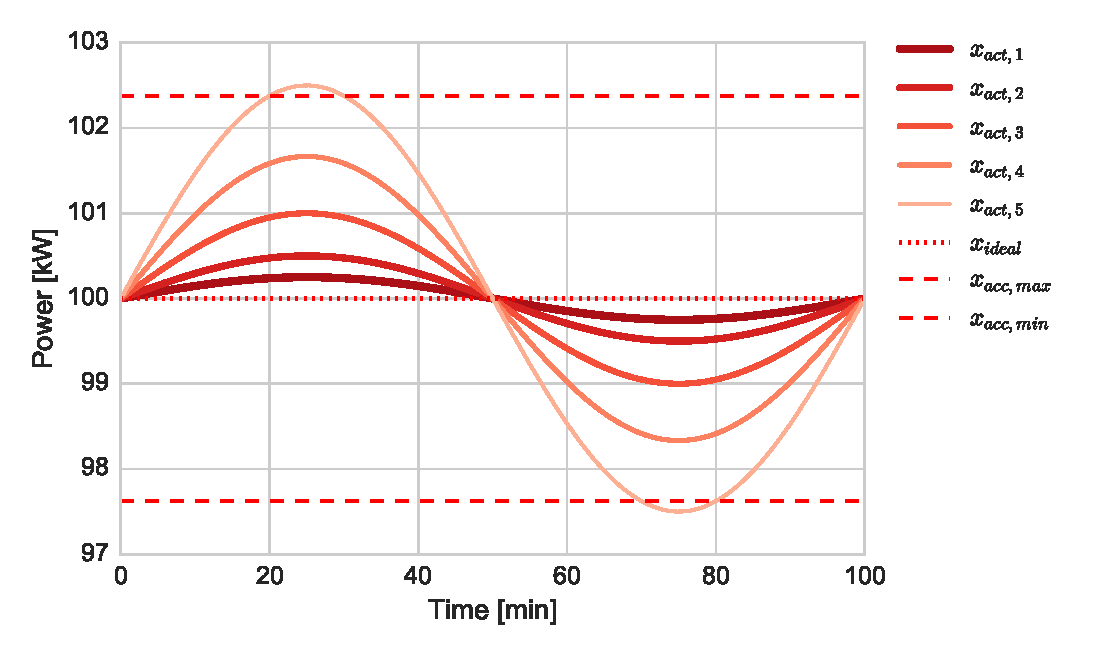
\includegraphics[width=1\columnwidth]{indextest_initial.eps}%
\label{subfig:indextest3}} \\
\subfloat[QoS for the services]{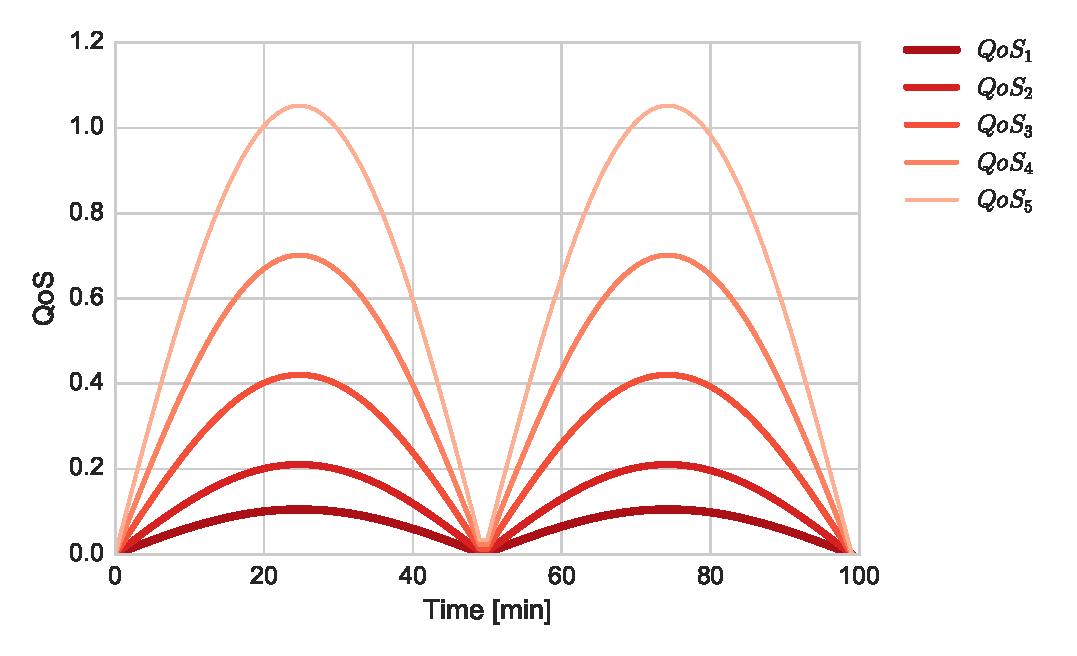
\includegraphics[width=1\columnwidth]{qostest_initial.eps}%
\label{subfig:qostest3}}
\caption[][1\baselineskip]{Test of the QoS definition where five aggregators deliver the same service for the same time horizons and with different performance.}
\label{fig:indextest3}
\end{figure}

\begin{margintable}%[-5\baselineskip]%[h!]
	\centering
	\begin{tabular}{cc}
		\toprule
		Aggregator & $\eta$ \\
		\midrule
		1 & 0.0740 \\
		2 & 0.1481 \\
		3 & 0.2962 \\
		4 & 0.4937 \\
		5 & 0.7308 \\
		\bottomrule
	\end{tabular}
	\caption{The values of $\eta$ for same service delivery horizons and different service performance.}
	\label{tab:qostest3}
\end{margintable}
%\FloatBarrier
The definition of $\eta$ takes the time horizon of service provision into account. This is done, so that the performance assessment gives a result that is scaled to the time scale of service delivery. For example, if two aggregators perform with an error of equal magnitude, but one aggregator is contracted to deliver the service on a shorter time horizon, the assessment of this aggregator should be worse than the one which was contracted for a longer period. This is shown in Figure~\ref{fig:indextest4} and Table~\ref{tab:qostest4}, where Aggregator 1 delivers the same service and the same error as Aggregator 2 but over half the delivery period.

\begin{figure}[htb!]
\centering
\subfloat[Simulated service delivery]{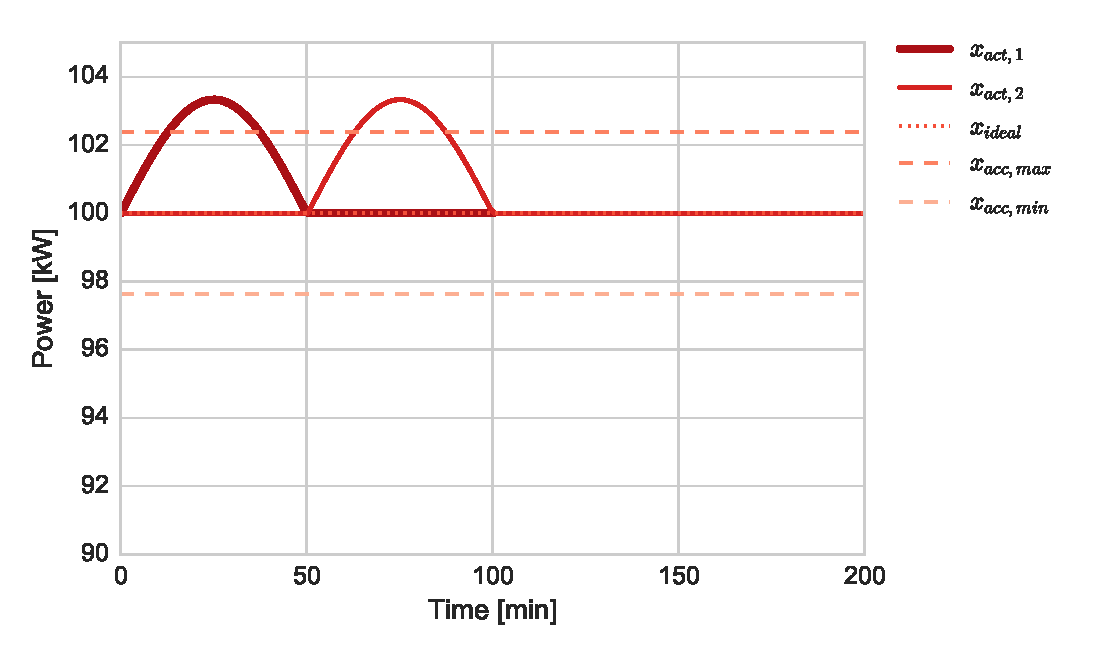
\includegraphics[width=1\columnwidth]{timenormtest.eps}%
\label{subfig:indextest4}}\\
\subfloat[QoS for the services]{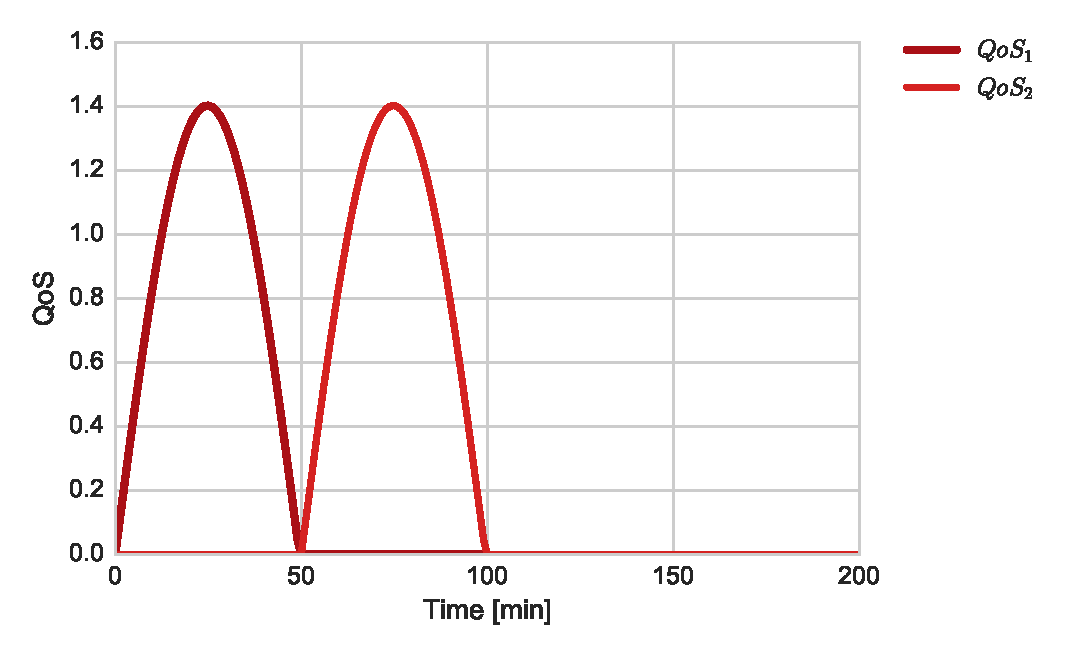
\includegraphics[width=1\columnwidth]{qostimenormtest.eps}%
\label{subfig:qostest4}}
\caption{Test of the QoS definition where 2 aggregators deliver the same service for different time horizons and with the same magnitude of error.}
\label{fig:indextest4}
\end{figure}

\begin{margintable}%[-1\baselineskip]%[h!]
	\centering
	\begin{tabular}{cc}
		\toprule
		Aggregator & $\eta$ \\
		\midrule
		1 & 0.3491 \\
		2 & 0.2469 \\
		\bottomrule
	\end{tabular}
	\caption{The values of $\eta$ for different service delivery horizons and with the same magnitude of error. Since $\eta$ is normalized with time, the shorter service is evaluated worse than the service delivered over the long time horizon.}
	\label{tab:qostest4}
\end{margintable}
%\FloatBarrier
Conversely, if two aggregators deliver a service on different time horizons and both have an error in service delivery which is \emph{proportionately} the same, the performance assessment will evaluate them to have equal performance. This is illustrated in Figure~\ref{fig:indextest1}, where five aggregators deliver a reference tracking service over different time horizons. All aggregators have the same proportionate error\footnote{This is ensured by using a sine as the ``actual'' performance of the aggregators, and each case is an extra period of the sine wave.} which leads to the same $\eta$, as can be seen in Table~\ref{tab:qostest1}. There is a slight increase in the values of $\eta$ due to numerical round off, which means that the precision of $\eta$ depends on the precision of the measurements. The amount of significant digits should be determined by the system operator or whichever entity is in charge of the service performance assessment.
\begin{figure}[htb!]
\centering
\subfloat[Simulated service delivery]{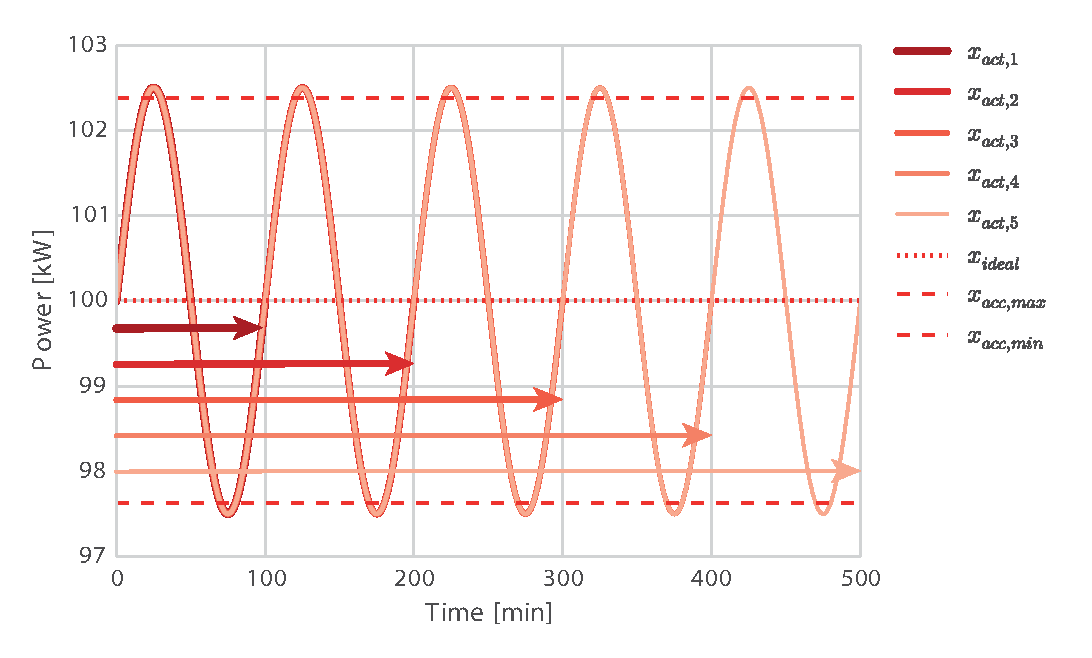
\includegraphics[width=1\columnwidth]{indextest_difftime_sameqos.eps}%
\label{subfig:indextest1}} \\
\subfloat[QoS for the services]{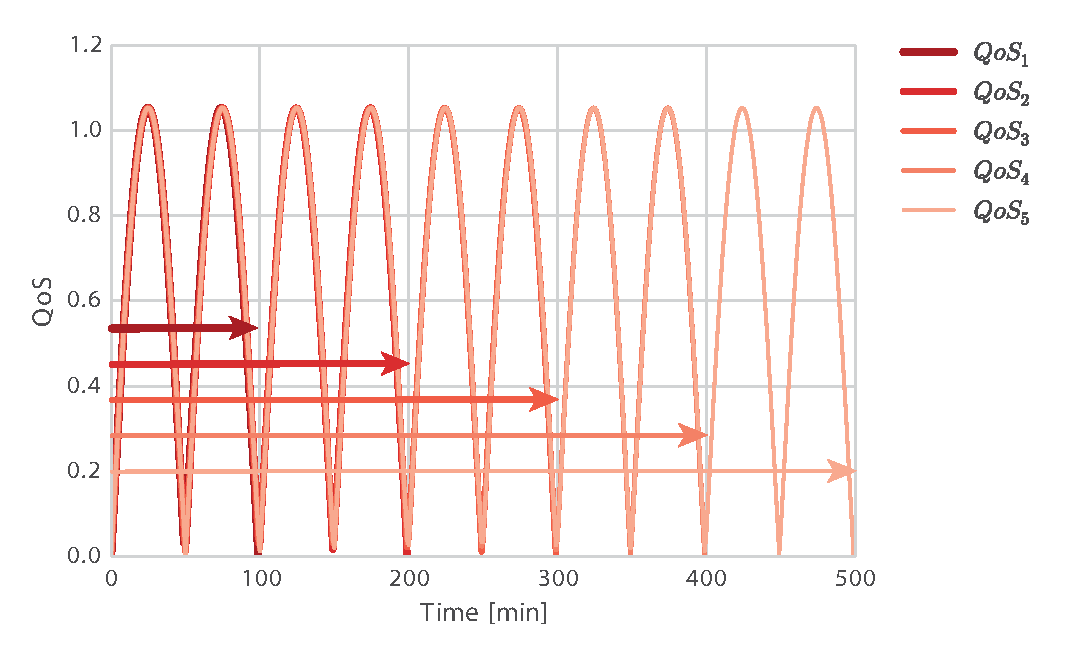
\includegraphics[width=1\columnwidth]{qostest_difftime_sameqos.eps}%
\label{subfig:qostest1}}
\caption{Test of the QoS definition where five aggregators deliver the same service for different time horizons and with the same performance.}
\label{fig:indextest1}
\end{figure}

\begin{margintable}%[15\baselineskip]%[h!]
	\centering
	\begin{tabular}{cc}
		\toprule
		Aggregator & $\eta$ \\
		\midrule
		1 & 0.7309 \\
		2 & 0.7327  \\
		3 & 0.7327  \\
		4 & 0.7333  \\
		5 & 0.7338 \\
		\bottomrule
	\end{tabular}
	\caption{The values of $\eta$ for different service delivery horizons. A numerical difference appears in the third decimal due to rounding error. The precision of $\eta$ depends on the measurement equipment of the flexibility asset.}
	\label{tab:qostest1}
\end{margintable}
%\FloatBarrier
Finally, Figure~\ref{fig:indextest2} and Table~\ref{tab:qostest2} show five aggregator delivering the same service for different time horizons and with different performance. It can be seen that truncating the \emph{QoS} when calculating $\eta$ means that $\eta$ alone can not be used for assessing if a service was delivered. Thus, the service verification index, described in the next section, must be taken into account in order to give a complete idea of service performance and delivery.
\begin{figure}[t!]
\centering
\subfloat[Simulated service delivery]{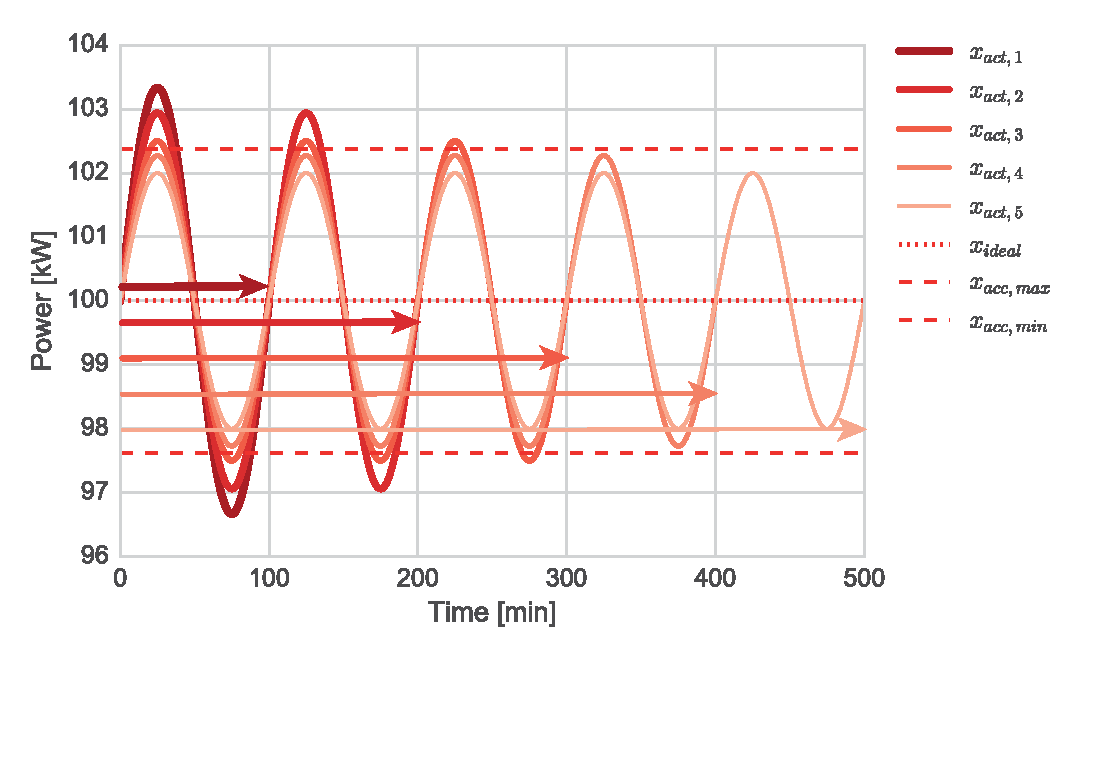
\includegraphics[width=1\columnwidth]{indextest_difftime_diffqos.eps}%
\label{subfig:indextest2}} \\
\subfloat[QoS for the services]{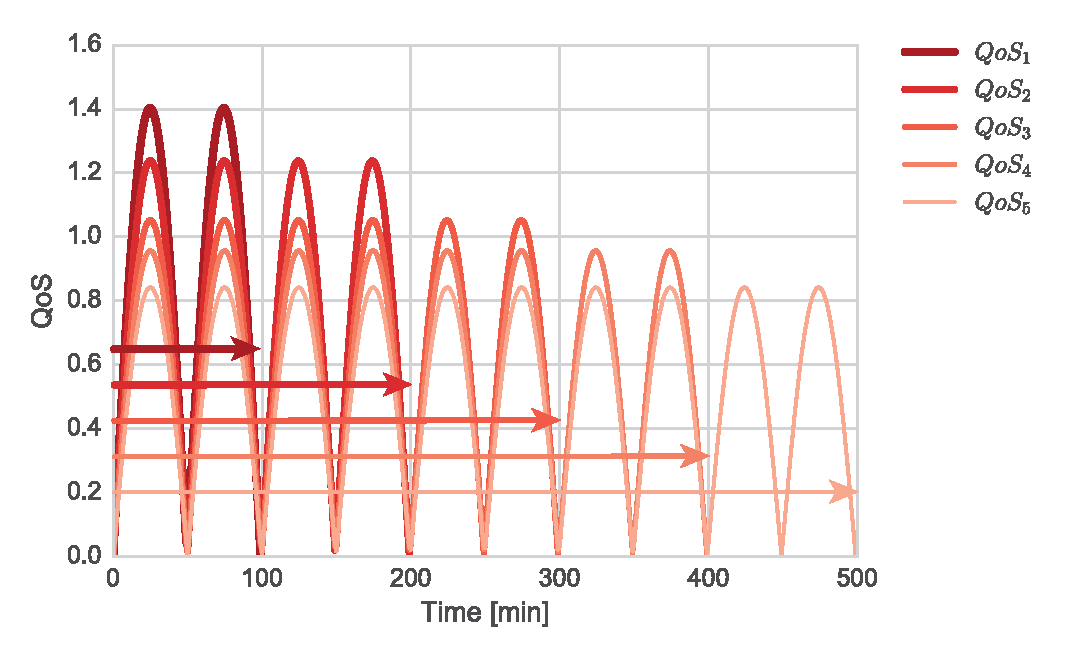
\includegraphics[width=1\columnwidth]{qostest_difftime_diffqos.eps}%
\label{subfig:qostest2}}
\caption{Test of the QoS definition where five aggregators deliver the same service over different time horizons and with different performance.
}
\label{fig:indextest2}
\end{figure}
\begin{margintable}%[-8\baselineskip]%[h!]
	\centering
	\begin{tabular}{cc}
		\toprule
		Aggregator & $\eta$ \\
		\midrule
		1 & 0.8199 \\
		2 & 0.7904  \\
		3 & 0.7333  \\
		4 & 0.6758  \\
		5 & 0.5949 \\
		\bottomrule
	\end{tabular}
	\caption{The values of $\eta$ over different service delivery horizons and different service performance.}
	\label{tab:qostest2}
\end{margintable}

%\FloatBarrier

\subsection{Service Verification Index}
Similar to the service performance assessment index, an index is defined for service verification\footnote{This index can also be interpreted as an index measuring non-delivery.} based upon \emph{QoS} whenever $QoS > 1$. A new non-delivery measure is introduced:
\begin{equation}
	ND(t) = QoS(t) - 1,\quad \forall QoS(t) > 1, \forall t.
\end{equation}
Using this new measure, the service verification index for \emph{K} amount of ancillary services, over a discrete time horizon of service delivery \emph{N}, is defined as:
\begin{equation}\label{eq:epsilonASmain}
	\epsilon^{AS} = \sum^{K}_{i=1} W^{AS}_i \sqrt{\frac{\sum^{N_i}_{t=0} \left( {ND^{AS}_{i,t}}^{2} \right)}{N_i}}
\end{equation}
where $\epsilon^{AS} \in [0,\infty]$ and $W^{AS}_i$ is the same as in Equation~\eqref{eq:was}. Similar to $\eta$, $\epsilon$ is also normalized to time.

The service verification for the index can also be defined for asset management services:
\begin{equation}\label{eq:epsilonAMSmain}
	\epsilon^{AMS} = \sum^{M}_{i=1} W^{AMS}_i \sqrt{\frac{\sum^{N_i}_{t=0} \left( {ND^{AMS}_{i,t}}^{2} \right)}{N_i}}
\end{equation}
where  \emph{M} is the size of the unit portfolio and $W^{AMS}_i$ corresponds to Equation~\eqref{eq:wams}. Following the definition of $\eta$, the verification index scales with time. This can be seen through the verification index values corresponding to Figure~\ref{fig:indextest1} in Table~\ref{tab:epstest1}. Again, due to numerical accuracy, only the second decimal number is significant.
\begin{margintable}%[h!]
	\centering
	\begin{tabular}{cc}
		\toprule
		Aggregator & $\epsilon$ \\
		\midrule
		1 & 0.0838 \\
		2 & 0.0839  \\
		3 & 0.0840  \\
		4 & 0.0840  \\
		5 & 0.0841 \\
		\bottomrule
	\end{tabular}
	\caption{The values of $\epsilon$ over different service delivery horizons with same delivery error, as shown in Figure~\ref{fig:indextest1}.}
	\label{tab:epstest1}
\end{margintable}

The two proposed indices have almost the same definition, the difference being that \emph{ND} is not truncated when estimating $\epsilon$. Table~\ref{tab:epstest2} shows the $\epsilon$ values corresponding to the example in Figure~\ref{fig:indextest2}, and shows clearly the definition of \emph{ND}, \ie values $QoS \leq 1$ are ignored, while $QoS > 1$ count as part of the non-delivery. Contrary to the service performance assessment index, the verification index does not have a clear limit for what is considered a verified serviced. For some services, \eg ancillary services, it is critically important that $QoS(t) \ll 1$, which would mean a requirement of $\epsilon \approx 0$. In other cases, $\epsilon > 0$ is tolerable to certain extent. The tolerance limit for $\epsilon$ should be defined in the contract agreements between aggregator and the entity acquiring the services.

\begin{margintable}[-5\baselineskip]%[h!]
	\centering
	\begin{tabular}{cc}
		\toprule
		Aggregator & $\epsilon$ \\
		\midrule
		1 & 0.3612 \\
		2 & 0.2512  \\
		3 & 0.0840  \\
		4 & 0.0  \\
		5 & 0.0 \\
		\bottomrule
	\end{tabular}
	\caption{The values of $\epsilon$ corresponding to Figure~\ref{fig:indextest2}.}
	\label{tab:epstest2}
\end{margintable}

%\begin{table}[h!]
%	\centering
%	\begin{tabular}{cc}
%		\toprule
%		Aggregator & $\epsilon$ \\
%		\midrule
%		1 & 0.3612 \\
%		2 & 0.2506  \\
%		3 & 0.0838  \\
%		4 & 0.0  \\
%		5 & 0.0 \\
%		\bottomrule
%	\end{tabular}
%	\caption{The corresponding values of $\epsilon$ to Figure~\ref{fig:indextest3}.}
%	\label{tab:epstest3}
%\end{table}

\section{Application to Service Verification}
\newsection{T}{he two indices defined} in the previous section have different applications. As stated in the introduction to the chapter, verification occurs at the prequalification phase, at the operation phase and at the settlement phase. The work during this project has focused on the use of the indices for prequalification and settlement. 

\subsection{Prequalification Verification}
In the case of prequalification, the indices form part of the assessment module of the validation framework presented in Figure~\ref{fig:MAINframework}. As such, the indices can evaluate the simulated results and return the $\eta$ and $\epsilon$ results. Since the simulations will be repeated enough times to gain a statistical certainty of the aggregator behavior, the verification of the simulated services will be a statistical value, \eg with a mean and a distribution.

\subsection{Settlement Verification}
Verification of delivered services occurs as a post-delivery analysis. For an aggregator, the verification of a delivered service will be done by the entity who bought the service, or a third party metering company. It is still an open question how the specific DER consumption/production will be measured, since in most cases the resource will be behind a common metering point, \eg the smart meter of a household. Also, current measurement requirements would force all resources to have expensive measurement equipment, of which the cost would far outweigh the profit of participating in the ancillary service markets. As part of an iPower demonstration event held at DTU Risø Campus in November 2014, a verification module was implemented, using the index definition of \cite{bondy2014performance}, for the verification of a DSO service. In this case, the consumption of the participating DER came only from flexible heating, and the measured consumption could be used to verify the service. An integration of the verification script to the code running the demonstration also showed that the same code could be used as a simple online performance monitoring tool.

\section{Conclusions on Performance Assessment}
The topic of performance assessment is important for the prequalification of aggregators, the monitoring of aggregator service delivery and the settlement of services. The presented indices are a tool that is useful for performance assessment. Although the concept of performance indices are not new in the power system, the established indices evaluate the overall system performance and reliability. While these indices provide a useful tool for system operators to evaluate their performance in maintaining a secure grid, they are not suited for the evaluation of aggregators. Therefore, the definition of these indices present a novel approach to the problem of evaluating the performance of aggregators.

A weakness in the presented work is that for verification of services, both indices must be used. The value of $\eta$ will always fall within the acceptable range $\eta \in [0,1]$ and it will be the value of $\epsilon$ which determines if the service is delivered. Still, $\eta$ gives an intuitive idea of how well the aggregator is performing within the limits stipulated within its service contract. $\epsilon$ does not have this same intuitive meaning, but in that sense it is not different from other fit measures used in statistics.

Future work will focus on a re-implementation of the verification module for the laboratory, incorporating the indices defined in \cite{bondy2016method}. Also, research must be done with respect to how to measure the individual DER consumption in an economically feasible way, with enough resolution to do settlement verification.
% chapter Service Verification (end)


%\blinddocument
%!TEX root = ../Thesis.tex
\chapter{Conclusion and Future Work}
\label{cha:conclusion}
\newchapter{M}{orbi pharetra ligula} integer mollis mi nec neque ultrices vitae volutpat leo ullamcorper. In at tellus magna. Curabitur quis posuere purus. Cum sociis natoque penatibus et magnis dis parturient montes, nascetur ridiculus mus. Suspendisse tristique placerat feugiat. Aliquam vitae est at enim auctor ultrices eleifend a urna. Donec non tincidunt felis. Maecenas at suscipit orci.
\section{Discussion of key results} % (fold)
\label{sec:Discussionofkeyresults}


Aggregator validation consists of three things:
\begin{itemize}
	\item Documentation through the reference architecture
	\item Simulation aided validation tests
	\item Communication test
\end{itemize}

% section Discussion of key results (end)

\section{Future Work} % (fold)
\label{sec:FutureWork}

% section Future Work (end)

\section{Application} % (fold)
\label{sec:Application}

% section Application (end)


\appendix
\chapter{A Functional Reference Architecture for Aggregators}\label{app:etfa2015}

\textbf{Authors:}\\
	Daniel~Esteban~Morales~Bondy\\
	Kai~Heussen\\
	Oliver~Gehrke\\
	Anders~Thavlov

\noindent
\textbf{Published at:}\\
Emerging Technologies and Factory Automation (ETFA), 2015 IEEE\\
Luxembourg, Luxembourg

\noindent
	\textbf{Abstract:}\\
Aggregators are considered to be a key enabling technology for harvesting power system services from distributed energy resources (DER). As a precondition for more widespread use of aggregators in power systems, methods for comparing and validating aggregator designs must be established. This paper proposes a functional reference architecture for aggregators to address this requirement.


\section{Introduction}
The increase of electricity production from fluctuating renewable sources is creating a need for new ways of operating the power system. Demand response (DR), i.e. the exploitation of flexibility in electricity consumption, is considered a promising technology for mitigating this problem. However, a significant part of the DR potential exists in distributed, small and medium-sized loads. It is not practical for a power system operator to interact directly with all these flexibility assets. The role of aggregators is the creation and management of a portfolio of flexibility assets and  representation of this combined flexibility to a system operator and/or market.

System operators today rely on generators for ancillary services to maintain reliable system operation. Generators undergo validation tests and continuous monitoring on the generator site. With ancillary services provided by aggregators, similar validation and performance requirements will have to be established. However, validation and monitoring requirements cannot effectively be translated from single site monitoring to distributed aggregator control systems, and today's on-site monitoring cannot be scaled to distributed flexibility assets. 

We propose a functional aggregator reference architecture that facilitates specification and validation of aggregator functional requirements and the generic modeling of contractual and verification performance requirements. Application of the proposed functional architecture to  different aggregator designs suggests it as a meaningful benchmark for technology maturity.

% SUGGESTING TO REMOVE THIS PARAGRAPH FOR THE SHORT PAPER
%The paper presents a short overview of the current state of aggregation in Section~\ref{sec:agginsg}. The motivation for the reference architecture are presented in Section~\ref{sec:requirements} and an analysis of the aggregator functionality is presented in Section~\ref{sec:funcdec}. Section~\ref{sec:refarch} presents the proposed framework based upon the functionality analysis, and Section~\ref{sec:applic} shows how the framework can be applied to a set of academic and commercial aggregators.

%usual blabla about Smart Grids, and which problems aggregators are supposed to address in the Smart Grid context (scalability/divide-and-conquer, threshold to market entry, competition and indirectly robustness because of multiple implementations etc.). 
%\begin{itemize}
%\item Commercial aggregators are being developed by multiple parties and see their first field use. All of these are one-off designs.
%\item Performance evaluation and service validation will become important issues to be solved once aggregators are supposed to leave the protected field test environment and enter a competitive market.
%\item However, the wealth of different designs and solutions makes finding a common benchmark for evaluation and validation difficult.
%\end{itemize}
%This paper proposes a generic reference architecture for the performance evaluation of aggregators which can be used for ... and makes ... easier.

%Also, this work can serve as a checklist for companies that seek to start an aggregator business.
%Aggregation of large quantities of small, medium sized loads or a few large loads is a solution for harnessing resources that are useful for maintaining power quality and reliability in power systems with large penetration of fluctuating renewable energy sources.


%#############################################
\section{Aggregation in Smart Grids}
\label{sec:agginsg}
%This is where the state of the art goes:
%\begin{itemize}
%\item what is aggregation in a smart grid context?
%\item What is being aggregated?
%\item What is the purpose of the aggregation (delivery of which product?) 
%\item Which types of design exist (examples, not categorisation yet - we'll do that later) Examples
%\item Outcome: Why are aggregators an issue in smart grids?
%\end{itemize}
We refer to the concept of aggregation as the  creation and (commercial and technical) management of a portfolio of flexibility assets with the objective of offering the combined flexibility as a commercial service. The business role and technical function of performing aggregation is referred to as the Aggregator. In literature and business context use of these and related terms is not yet harmonized.
\begin{figure}[t!]
\centering
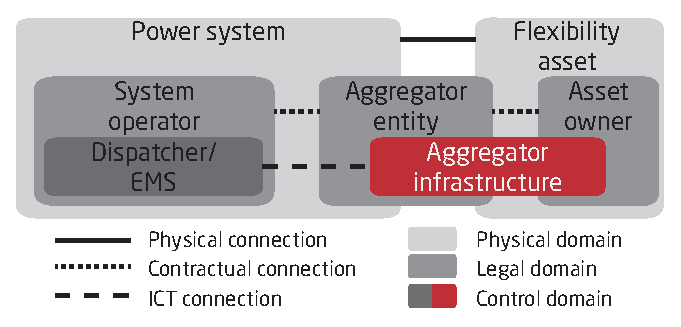
\includegraphics[width=1.0\columnwidth]{etfa2015/domains.eps}
\caption{The aggregator concept across domains.}
\label{fig:domains}
\vspace*{-5mm}
\end{figure}
\subsection{Clarifying the Aggregator concept}\label{subsec:clarifying}
The term \emph{aggregation} has different relevant interpretations in business, information technology,  control, as well as in the physical power system domain. Our concept of aggregators is illustrated in Fig.~\ref{fig:domains}, defining aggregators as a business role, aggregator entity, as well as a technical aggregator infrastructure.

The physical domain addresses the electrical interactions between flexibility assets (also referred to as DER) and power system. Whereas aggregation with respect to physical topology is a common concept (e.g. microgrids, cells), in our understanding, aggregators are not bound to aggregation with respect to physical network topology. 
%The aggregator is only reflected in this level by the manipulation of the interaction between the flexibility assets and the power system.

In the legal and business domain, an aggregator entity is an intermediary, maintaining contractual relations with flexibility asset owners and system operators (as receivers of flexibility services). The aggregator entity assumes legal responsibility for the delivery of a contracted service. The aggregator role may be filled by new independent market actors or be part of existing actors, such as utilities or balance responsible parties.

In the control domain, the aggregator infrastructure coordinates the behavior of flexibility assets. The control domain requirements are formulated as \emph{flexibility services} to system operators and \emph{asset management services} towards asset owners. Tracing these requirements for architectural validation and performance validation in the aggregator infrastructure is the focus of this paper.

The proposed aggregator concept is implementation agnostic and focused on formulation of functional requirements.

\subsection{The aggregator concept in technical literature}
There is no unanimous definition in literature of what could be considered standard functionality of an aggregator. This is reflected by the wide variety of aggregator designs\fcite{kok2005powermatcher,han2010development,sortomme2011optimal,costanzo2013coordination}, which differ in capabilities and purpose, and which use different (often implicit) criteria for classification.

Aggregators are commonly classified by control scheme into autonomous, indirect, transactional and direct control \fcite{Kosek}. Another classification emphasizes the commercial or technical focus of aggregators, referring to \emph{commercial} and \emph{technical} virtual power plants (CVPP and TVPP) \fcite{fenix2009}; however, as both types require business and technical functionality, the CVPP/TVPP distinction expresses a difference in degree and is not categorical. An advanced aggregator realizing the full functionality spectrum as \emph{Dynamic VPP} (DVPP) has been formulated in other work\fcite{niesse2014conjoint}. 
The proposed concept of aggregation encompasses all of the above but focuses on functional requirements for service provision, not business logic.

\subsection{Aggregator Business Harmonization and Standardization}
Whereas aggregator functionality is becoming a shared concept, there are still many models describing a) which stakeholders may benefit from the flexibility service, b) the form of the flexibility service, c) which stakeholders (are allowed to) perform aggregation and who should receive compensation \fcite{eurel-aggr} and d) how to harmonize the interaction between aggregators and aggregated units.

With respect to a), market models are being revised and new service models introduced to assign a value to flexibility (either directly to system operators as ancillary service, or as enhancement of flexibility of existing portfolios). The form of the service, b), is often formulated as an abstract flexibility service, a trade-off between both grid needs and generalized resource characteristics. Regarding d), many aggregators use proprietary communication, loosely based on standards (e.g. IEC61850 or IEC 60870-5-104; increasingly also OPC-UA); harmonization efforts in Europe continue to be addressed in the Smart Grid Coordination Group (SGCG) under EU Mandate M/490. A successful interoperability effort in this domain is the OpenADR standard published also as IEC PAS 62746.10-1. Meanwhile the IEC TR 62357 \emph{Reference Architecture to Smart Grid Information Exchange} is under revision. The reference architecture presented here focuses, within the Smart Grid Architecture Model\fcite{SGAM}, on functional interoperability for aggregators (field to operation zones; DER and customer domains) supporting interactions with System Operators, market actors, and devices at process level.

%\noindent\rule{4cm}{0.4pt}\\
%\textcolor{red}{(the follwoing defintioins belong into this section)}\\
%DEFINITION\\
%LEGAL\\
%Aggregator Role $\surd$\\
%Flexibility Asset Owner Role $\surd$\\
%SOFTWARE DOMAIN\\
%Virtual Nodes  (agents, processes) $\surd$ \\
%aggregator-side $\surd$ \\
%asset-side $\surd$ \\
%PHYSICAL DOMAIN \\
%Aggregator Site\\
%Flexibility Asset $\surd$ \\
%Device Interface $\surd$ \\ 

%#############################################
\section{The Need for an Aggregator Reference Architecture}
\label{sec:requirements}
%The power system is experiencing a paradigm shift. 
Existing concepts and methods for benchmarking and generator validation/certification cannot readily be translated from the (bulk) generator based paradigm to the distributed paradigm of aggregators and flexibility services. Historically, ancillary services have been defined using a physical understanding of generator capabilities. This definition is moving towards technology-agnostic service models.
Service verification has been done through on-site measurements, which is infeasible with thousands of units participating in service provision.  

The definition of a reference architecture for aggregators addresses these three issues, and enables benchmarking of aggregator architectures.
A reference architecture ``captures the essence of existing architectures, and the vision of the future needs and evolution to provide guidance to assist in developing new system architectures.''\cite{cloutier2010concept}. It should provide: 
\begin{itemize}
\item a common lexicon and taxonomy,
\item modularization and the complementary context, and
\item a common (architectural) vision.
\end{itemize} 

%1) new industry -> benchmark, kpis certification is needed, since they cannot be translated from the old industry 
%
%2) service verification is different -> traditionally expensive measuring equipment. new method is needed for new architecture
%
%3) technology agnostic service models, rather than technology based services. Need an architecture to standardize context
%The common lexicon and taxonomy allows for precise discussion and a common understanding of what an aggregator is and can do. The establishment of these two concepts is started in Section~\ref{subsec:clarifying}, where the context of the aggregator is also discussed.% and further refined throughout the paper. 
Various types of aggregator implementation exist, realizing different design ideas for different sets of requirements. These requirements -- and consequently the designs derived from them -- are unlikely to converge towards a single solution because of the tradeoffs involved, e.g. scalability and complexity. A common lexicon and taxonomy is a minimal precondition for aggregator comparison.
If a reference architecture is to be used to describe many of these different designs, it must be highly modular. In practice, the \emph{general} functionality of an aggregator must be broken down into small enough functions in order for these functions to be usable as building blocks for the reconstruction of the \emph{particular} functionality of a given implementation. 
The functions are arranged in a reference architecture such that metrics can be assigned to individual functions. In this way, the reference architecture can be used for validation of the aggregator. Our architectural vision accounts for the need for verifying distributed flexibility services.

%Implementability (discuss what that means in this context?)

%The methodology for the analysis is the following:
%\begin{itemize}
%	\item We have analyzed different aggregator architectures from the literature, as well as the experience gained through the practical implementation of an aggregator in our laboratory, and extracted the essential functionalities necessary for the working of the aggregator. These functionalities are independent from aggregator/control architecture.
%	\item We analyze the functions and their relationships, as well as the level of complexity we can foresee.
%	\item Synthetize the results into a reference architecture. 
%	\item Validate by mapping different architectures into the framework.
%\end{itemize}


%This is still part state of the art, so this and the previous section together shouldn't be too long)
%\begin{itemize}
%\item \textit{The method}
%\item Why would somebody want to evaluate aggregator performance?
%\item Which methods/approaches for performance evaluation exist or are being discussed?
%\item What is missing? (A reference architecture of course, but why?)
%\end{itemize}

%#############################################
\section{Functional decomposition}
\label{sec:funcdec}
An aggregator is a complex system of interacting functions. In the following definitions, we abstract from implementation details, e.g. centralized vs. distributed systems, and focus purely on the purpose of the functions. 

% EXTERNAL INTERFACES
%\subsection{Service Interface}
\textbf{A. Service Interface}
The service interface translates the contractual agreements between the aggregator and its clients into a service model containing quantifiable and measurable service requirements and a set of performance criteria. This service model is then used to map incoming service requests to control domain signals such as control variables, constraints or control parameters.


% Monitoring & Supervision modules
%\subsection{Performance Monitoring}
\textbf{B. Performance Monitoring}
The performance monitoring function collects data from which the behaviour of individual clients can be derived. The data is analyzed to determine the performance of a client, and its compliance with the contracted flexibility service. This analysis may be internal to the performance monitoring function, or it may simply serve as a data gatherer for an external entity.


%\subsection{Supervision and Resource Handling}
\textbf{C. Supervision and Resource Handling}
The aggregator must maintain an overview of available client resources and their status. By comparing the communication status and monitored performance of individual clients to the control signals sent by the aggregator, the supervision function determines whether clients perform according to their contract. It may temporarily or permanently exclude non-compliant clients from the pool of available resources.


%\subsection{Operator Interface}
\textbf{D. Operator Interface}
Although the power system is moving towards automated solutions, decision-making on critical issues is the responsibility of human operators. The aggregator architecture must support decision-making by presenting operators with the necessary information, and facilitating operator input and intervention.  %\textcolor{red}{(Incomplete/rewrite!)}


% Control-related
%\subsection{Control}
\textbf{E. Control}
The control function is in charge of generating the appropriate control domain signals for the portfolio. Depending on the control architecture, the control logic may be distributed between physical entities. The concept of a control domain signal covers several kinds of signals, including, but not limited to control inputs to DERs, coordination messages for distributed control and reference signals for hierarchical controllers.


%\subsection{Flexibility Monitoring}
\textbf{F. Flexibility Monitoring}
In operation, the aggregator must assess the future flexibility of its portfolio in real time; this includes individual DER flexibility as well as the aggregated flexibility of the portfolio. The flexibility assessment can either be based on direct feedback from the DERs or entirely on estimation models (possibly stochastic) if direct feedback is not available.

% Communication
%\subsection{Aggregator-internal communication}
\textbf{G. Aggregator-internal communication}
Except for very few special cases, aggregation will almost always be implemented as a distributed computing system. In its basic form, such a system would consist of one aggregator and a number of clients. This may be extended by stacking multiple levels of aggregation etc. The internal communication function exchanges information between aggregator and clients.


%\subsection{Client management}
\textbf{H. Client management}
The client management function actively or passively tracks the availability of clients. It may also provide a mechanism for the dynamic addition and removal of clients, such as a discovery service, and maintain a protocol for temporarily disabling otherwise available resources. It contributes to resilience and graceful degradation of the portfolio.



%\subsection{External Information Services}
\textbf{I. External Information Services}
To be able to act optimally with respect to both control of its portfolio and trade of electricity in forward markets, aggregators will likely have to rely on different types of information services. Such services include different types of forecasts and measurements in real time and may be provided by either internal processes or by a 3rd party. 


%\subsection{Asset interface}
\textbf{J. Asset interface}
Most aggregators in a Smart Grid context will be used to harvest flexibility from existing energy resources. In most cases communication between aggregator and resource will use a fieldbus-style interface not designed for wide-area communication. The purpose of the asset interface is to maintain communication with a physical unit under aggregator control and provide abstraction from interface details.


% the odd one
%\subsection{Information Exchange}
\textbf{K. Information Exchange}
Virtually any modular software framework contains a facility for information exchange between its components and storage of the overall system state: static data, dynamic data or both. A knowledge exchange may take many different forms, from a collection of object references towards a central or distributed database. 


%#############################################
\section{The Reference Architecture} 
\label{sec:refarch}
% === This is where we collect the knowledge collected in the previous section into the actual architecture and discuss it and its building blocks. (Introduce complexity levels) ===

We have now established a set of functions to serve as building blocks for a reference architecture, but without concern for the relations between these blocks. Next, these relations will be examined; in other words: how could a practical aggregator infrastructure be composed from these function blocks?

\subsection{Function blocks and knowledge exchange diagram}

% === Explain what the function blocks symbolize - and how the location in the function block diagram does not say anything about whether a block exists on the aggregator side, the client side or both. ===

The functions in section \ref{sec:funcdec} generally belong to one of the following categories:
\begin{itemize}
\item functions dedicated to communication between physically separate parts of the aggregator infrastructure or communication with 3rd party entities, i.e. enablers of the distributed nature of the system.
\m functions which perform decisions with regards to flexibility asset behavior and portfolio composition.
\item functions which interpret information and support the decision making functions. 
\end{itemize}
These categories represent requirements for different architectural paradigms: Communication functions are layered or hierarchical, and, in the case of communication between aggregator and client, require an identically layered counterpart at the opposite end. The decision making and interpreter functions on the other hand require many hierarchical and non-hierarchical consumer-producer relations. % The interpreter functions generally exist in direct relationship with the decision making functions. %The knowledge exchange function, storing the different elements of system state, provides a link between these two worlds.  
Figure~\ref{fig:functiondiagram} shows an overview of the relationships between functions according to the above concept.

\begin{figure}[htb]
\centering
\includegraphics[width=1.0\columnwidth]{"etfa2015/diag_simple"}
\caption{Each function outputs distinct kinds of data which are used by the other functions in different ways according to the aggregator implementation.}
\label{fig:functiondiagram}
\end{figure}

\subsection{Principles of distribution of functions}

While figure \ref{fig:functiondiagram} depicts the relationship between aggregator functions, it does not include information about the physical distribution of these functions between the asset side and the operator side of the aggregator infrastructure. This distribution is highly specific to the individual design and e.g. its degree of centralization (see section \ref{sec:applic}).

In an actual implementation, several of these functions require corresponding instances on each side, effectively forming a communication stack. 

The functions exhibiting these properties are:
\begin{itemize}
\item the internal aggregator communication function which provides the link between the two substacks. In many cases, this function will make use of a full OSI-layered stack in which the internal aggregator communication function provides the application layer,
\item the client management function, implementing management protocols which would typically require a corresponding instance on the client side, and
\item the knowledge exchange function which exchanges information with its client side counterpart independent of client management mechanisms.
\end{itemize}

All other functions, with the exception of the asset interface, may appear either on the operator side, on the asset side, or shared between both sides, depending on the implementation.

%#############################################
\section{Case studies} 
\label{sec:applic}

A number of existing aggregator designs -- commercial as well as academic -- have been mapped to the model in order to test its viability. Two cases with different design philosophies are presented here in order to illustrate the distribution of functionality between the operator and the asset side, and the information flow between the functions:
\begin{itemize}
	\item \emph{Power Hub} is an aggregator developed by Dong Energy in Denmark. It is used to control distributed generation and load in order to sell flexibility services to the ancillary power market (Figure~\ref{fig:powerhub}).
\item \emph{Open Energi} is a British company selling flexible consumption from industrial loads as an ancillary service. The aggregator functions are distributed between an operator node at a control center and asset nodes on custom hardware deployed at customer sites (Figure~\ref{fig:openenergi}).
\end{itemize}

The most significant difference between the two designs is the degree of autonomy of the asset node. The Power Hub concept is based on a centralized design which mainly uses the asset node as a communication gateway and places flexibility monitoring and control at the central operator site. This is also where external information such as market data is available through the information services function.
The Open Energi controller acts on quantities measurable at the asset site and does not require external information; this allows control and flexibility monitoring to be placed at the asset node, leaving only supervisory functions at the operator site.

Both designs can be split into functions according to the subdivision proposed in section \ref{sec:funcdec}.

\begin{figure}[htb]
\centering
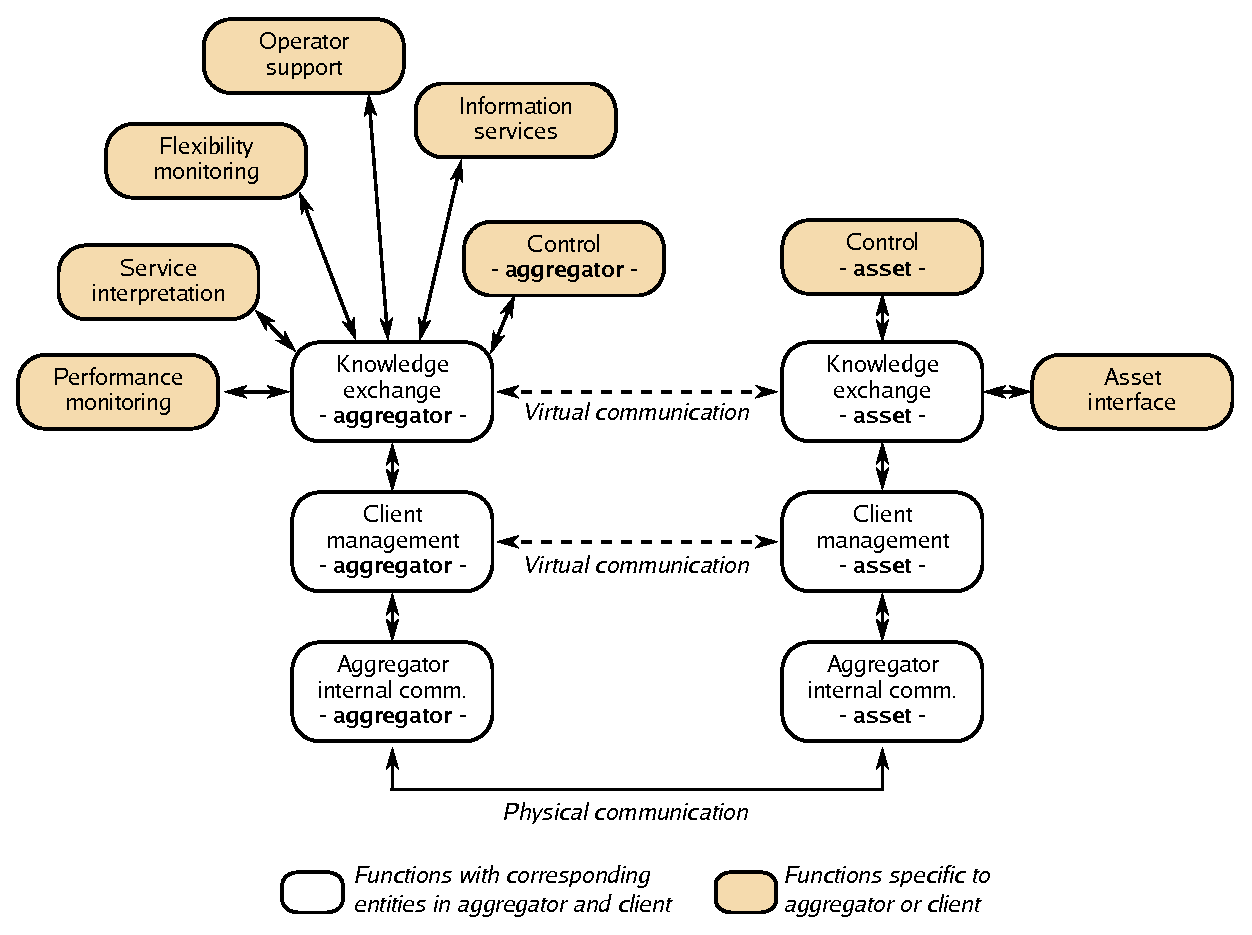
\includegraphics[width=0.65\columnwidth]{etfa2015/stackdrawing_powerhub.eps}
\caption{Distribution of functions for the Power Hub aggregator}
\label{fig:powerhub}
\vspace*{-5mm}
\end{figure}
\begin{figure}[htb]
\centering
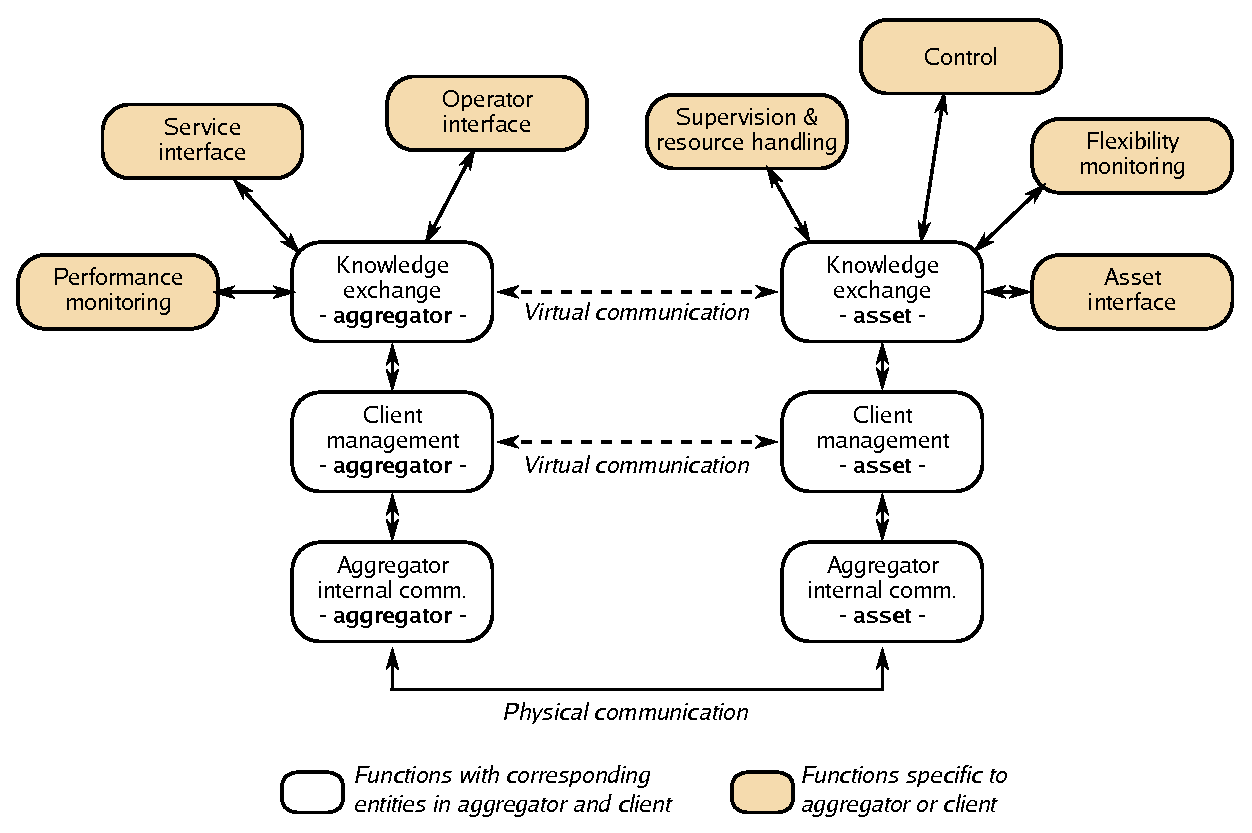
\includegraphics[width=0.65\columnwidth]{etfa2015/stackdrawing_openenergi.eps}
\caption{Distribution of functions for the Open Energi aggregator}
\label{fig:openenergi}
\vspace*{-5mm}
\end{figure}



%#############################################
\section{Conclusion and further work}
\label{sec:etfa2015:conclusion}
A reference architecture for the validation and comparison of aggregators has been presented. While the general framework has been established and successful mapping tests to a number of real-world aggregator designs have been performed, many details are still work in progress.
The next steps towards completion will be the development of performance indicators for the individual functions and the establishment of a process for aggregator comparison and performance validation.

%Review 1: As the goal of the paper is to develop a reference archcture, please elaborate on reference architectures in general and on the SGAM in particular.

%
%Review 2: The WIP-paper presents a high-level reference archcture for the validation and comparison of aggregators for power system services from distributed energy resources. Based on a functional decomposition of practical implementations a reference architecture is developed. It is validated against two practical implementations (power hub and open energi). 
%
%The value of a reference archcture for the crucial role of aggregators such as this is obvious but the developed architecture needs to be validated with more practical examples. How and if this architecture may be used performance evaluation, comparison or even optimization of aggregators remains to be proven. But the paper definitely meets the requirements of a WIP contribution.

%Review 3:	The concept of the reference archcture is nicely introduced and explained. Since it is a work in progress paper a more detailed presentation of future work would be appreciated.

%#############################################
\section*{Acknowledgment}
Parts of this work are supported by the Programme for Energy Technology Development and Demonstration (EUDP) and Innovation Fund Denmark through the iPower project.


\chapter{Validation of Aggregators Providing Demand Response}\label{app:pscc2016}

\textbf{Authors:}\\
Daniel Esteban Morales Bondy\\
Oliver Gehrke\\
Anders Thavlov\\
Kai Heussen\\
Anna M. Kosek\\
Henrik W. Bindner

\noindent
\textbf{Submitted to:}\\
Power Systems Computational Conference, 2016 \\
Genoa, Italy


\noindent
\textbf{Abstract:}\\
As aggregators become viable sources of ancillary services, they will be required to undergo a validation process similar to the prequalification process of traditional generators. Since aggregators are fundamentally different from traditional generators, a new test method must be designed for the aggregator validation. This work proposes a method for designing the tests necessary for the validation process. The method is exemplified with a study case and results are presented.
\section{Introduction}
As renewable energy generation increasingly replaces conventional power plants, power system operators are looking for alternative sources for the ancillary services which were traditionally provided by these plants. It is expected that some ancillary services can be procured from distributed consumption and production units by making use of their unused operational flexibility. In order to provide coordinated services, such as demand response \cite{macdonald2012demand}, from a large number of such distributed energy resources (DERs), a new actor is appearing in the power system: the aggregator \cite{gkatzikis2013a}.% \hl{I was wondering whether we should clarify which type of aggregator we're talking about here, to make it harder for nitpicking reviewers.}\textcolor{red}{You mean commercial VPP vs Technical VPP?}

Conventional sources for ancillary services must be certified before being able to offer control reserves in an ancillary services market \cite{energinet2012ancillary}. It is expected that aggregators will be required to undergo a similar prequalification process to ensure the appropriate performance of the provided service with respect to predefined requirements.

The achievable performance of aggregators, in terms of service provision, depends on its architecture \cite{bondy2015a}, i.e. where the decision making is located \cite{kosek2013overview} and its level of automation, the choice of hardware for implementation, the specification of communication protocols \cite{kiliccote2010open}, how advanced the portfolio management is, etc. This means that some aggregator architectures will be better suited for a specific ancillary service than others \cite{bondy2014performance}. 

It has been established that current requirements for participation in the ancillary services markets limit the participation of aggregators of demand response \cite{cappers2013assessment,coalition2014mapping}. Different research projects have looked into this problem, see e.g. \cite{bondy2014flech}. 

Until now, the performance evaluation and testing of aggregators in academia has been ad-hoc to specific aggregator implementations \cite{vrettos2015integrating,rahnama2014evaluation}. Aggregator test frameworks have been proposed \cite{buscher2015towards}, field tests have been carried out in order to validate DR schemes \cite{kiliccote2013field}, and concepts regarding systematized testing have been exemplified \cite{steinbrink2015challenges}.

This work addresses the gap between all these concepts, i.e. we present a procedure for the design of validation tests, which takes a systematical approach to aggregator testing, discussing the issue from input, i.e. service requirements, to output, i.e. performance metrics.

%This work addresses the gap between all these concepts, i.e. the design of a test procedure that takes a systematical approach to aggregator testing, discussing the issue from input, i.e. service requirements, to output, i.e. performance metrics.

%Therefore new methods and tools are needed to validate an aggregator architecture, in terms of capability to deliver the desired services. %Such an assessment of an aggregator can be relevant before investments into a particular infrastructure are made. The methods may also be incorporated into an aggregator prequalification process.

%The purpose of this paper is to derive the testing specification for an aggregator from its contracted service requirements. Specifically, we constrain the analysis to active power services such as frequency containment and frequency restoration reserves \cite{entso1operational} for transmission systems and congestion management for distribution systems. The novelty presented in this work is a method for designing validation tests for aggregators. \hl{How can I give this more oomph?!}

%of the interaction between the systems interacting directly or indirectly with the aggregator. \textcolor{red}{The word interaction is used too much here, how do I fix this?}\hl{I'm not sure if I know what you want to say. "testing of the interaction between the systems interacting with the aggregator" - what interacts with what here? My best bet right now is "The purpose of this paper is to describe the alignment of service requirements with the testing specification of the aggregator, including the interaction between its subsystems." Is that what you meant?}


\section{Conventional resource validation and aggregator differences}\label{sec:PSSCCconventionalvalidation}
%\hl{ We explain why system operators want resources to be validated (WHY?) }
Ancillary services are essential for the reliability of the power system. Because these services play such an important role in the safe operation of the system, it is important that the units or entities providing a service perform according to the requirements set by the Transmission System Operator (TSO). These requirements and processes are typically specific to a particular TSO and influenced by national regulations, interconnection grid codes etc. We will discuss two examples below:

In Denmark, energinet.dk, the Danish TSO, ensures this by requiring all units participating in the ancillary service markets to provide a documentation of their capabilities and go through an approval process \cite{energinettender}. This approval process consists of a test conducted at least three weeks prior to the service delivery date. The tests for Frequency Containment Reserve generally involves the injection of a setpoint step into the plant's governor and the measurement of the response. The test for Automatic Frequency Restoration Reserve involves the tracking of a reference signal from energinet.dk. Currently, this procedures are not formally described.
Demand resources are expected to provide a substantial amount of the ancillary services for the Danish grid in the future. Since distribution system services are not widespread yet, the concept of unit certification is non-existent at the distribution level. 

%\hl{Here we explain the current method for resource validation. (HOW?)}
%\hl{There is abig jump form Demnark to US, maybe we can sat that Denmark has not such regulations and US is more advanced in the process...}
While Denmark is starting to open up to new sources of ancillary services and standardise its test procedures, PJM (a regional transmission operator in the United States) has a standardised prequalification procedure for regulating resources\footnote{Regulation in the US corresponds roughly to frequency restoration reserves of ENTSO-E.}, which consists of three consecutive area regulation tests, where PJM Performance Compliance scores indicate how well the resource follows a simulated regulation signal. A single test lasts for 40 minutes and in order to pass it the unit must score at least 75\% in three consecutive tests \cite{pjm2015balance}. While this rule includes services provided by multiple generators at a single site, operators of demand resources are not required to be certified but must complete an initial training module on the requirements and business rules of the Regulation and Synchronized Reserve markets \cite{pjm2015certification}. Currently demand resources are only allowed to form 25\% of the total regulation \cite{pjm2015ancillary} in PJM, and therefore their certification process is still not a large concern. 

In both systems the validation tests have two goals: to ensure the communication with the units works correctly, and to validate the known performance model of the generators. Thus, a change of configuration in the setup requires a new certification of the generator.
%\hl{We show in which way the current method is not applicable to aggregators and other distributed / multi-resource service providers, and conclude that an alternative method is needed (WHAT?, problem statement)}

The current tests outlined above are specific to system operators (here, e.g. Energinet.dk and PJM), but follow similar paradigms. 
The conventional test processes outlined above cannot be directly applied to portfolios of aggregated resources, mainly because a common assumption in the process is that the service delivery is performed by a single or small number of units. This allows inference of the unit's ramping capabilities through a response test, based on a known model. 

An aggregator and the portfolio of units under its control behave fundamentally different from large generation units:
\begin{enumerate}
\item Individual generator units are well understood and models describing their static and dynamic properties are readily available. This is not the case for portfolios of aggregated units which are typically heterogeneous and can only be modelled through their statistical properties. This is aggravated by the fact that unit portfolios may be dynamically reconfigured during operation.
\item There might not be a meaningful equivalent to a single point of measurement: An aggregator's portfolio may consist of geographically dispersed units. Their aggregate power profile does not correspond to a measurement at any single point of the grid.
\item Aggregators, by definition, operate a distributed system (both in control and geographical terms) in which each unit has its own response properties and requirements. This leads to an aggregated response that behaves differently from that of conventional generators.
\item Reliability concepts for distributed systems are different; specifically, the failure modes are not the same. If a component of a monolithic generator unit fails, the whole unit may have to shut down. The failure of a single unit in an aggregator portfolio will often have a minor or negligible impact on the overall performance. In a large portfolio it will usually be possible to recruit an equivalent replacement unit providing the same services as the failed one.
%\item There are many different ICT and control architectures for aggregators, and interoperability standards must be used for the internal workings of the aggregator. \hl{and whats the point?}
%\item The primary purpose of units composing an aggregator is to serve a specific energy-dependent need of the unit owner, not to provide the flexibility service, hence not all units in an aggregator portfolio may always be available.\hl{This is a property of e.g. demand response, not of aggregation. It applies to a single DR unit as well. I'd skip this argument.}
\end{enumerate}

For the above reasons, validation cannot be performed on the individual units in an aggregator's portfolio, but has to be applied to the aggregator's control process and portfolio. This paper focuses on the alignment between service requirements and the design of the tests needed for the validation of aggregators. 

%is not as straightforward for aggregated systems due to their geographical distribution, dynamic nature, complex ownership structure, and possible difference between the service requirements of individual units and the aggregate as a whole.
%The service requirements may also differ between demand response and traditional ancillary services, which leads to different validation requirements.\textcolor{red}{better?}

\section{Requirements and proposed test  procedure}\label{sec:metrics}
%\hl{- What alternative method do we propose?}

The objective of the current tests is to validate the parameters of a well understood model of generation units. For the reasons stated previously, the new tests need to identify an empirical behavior model of an uncertain and diverse entity: the aggregator control architecture and unit portfolio. 

%This means that there is no single standard test, but 
A test procedure is required that will allow the system operators to understand and predict the performance of a specific aggregator under a given set of operation conditions (Fig.~\ref{fig:framework}). In this section we present the underlying assumptions for such a procedure, the metrics used to measure the aggregator performance, and the proposed procedure.
%Getting an empirical model of an unknown entity rather than a mathematical model of a known entity. System identification approach.

\begin{figure}[!t]
\centering
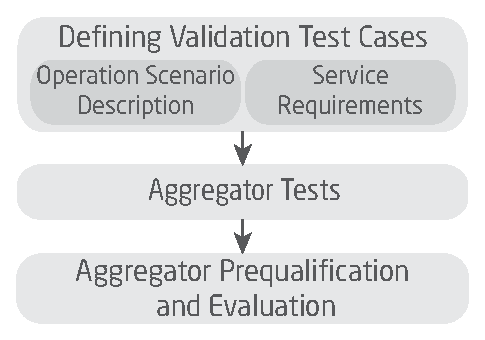
\includegraphics[width=1.7in]{graphics/pscc2016/validation.eps}
\caption{Schematic procedure for aggregator validation. The focus of this paper is on the relationship between the service requirements and the aggregator tests.}
\label{fig:framework}
\end{figure}

%Here the following three topics must be discussed:
%\begin{itemize}
%\item Boundary conditions (grid, DER)
%\item Fault scenarios
%\item Operation spectrum (what is the possibility/range of the input data?)
%\item Experimental design
%\end{itemize}

%The experiments should be able to measure response/states that can't be measured safely/easily under deployment.

%The tests must have a well defined input and output.

\subsection{Test Procedure Assumptions}\label{subsec:assumptions}
%A great variety of aggregator architectures has been proposed and implemented; differences between them are linked to specific business cases, local regulations, grid codes etc. Implementation details such as algorithms for portfolio composition, resource prediction or trading, constitute key intellectual property of commercially operating aggregators and disclosure of these business secrets will be unacceptable in many cases. For this reason,
The critical assumption are:

1) A general test design must start from the assumption that the aggregator and its infrastructure are to be treated as a black box, in the sense that only the aggregator inputs and outputs are known but the details of the internal control architecture are unknown.

%Field tests have been carried out in order to validate DR schemes, see e.g. \cite{kiliccote2013field}. While these kind of tests are important to characterize the capabilities of aggregators, the tests are not able to fully identify their operation capabilities. Thus, i
2) In order to fully test aggregators under a number of relevant scenarios, and to capture the stochastic nature of their operation, aggregators must be tested with the aid of a simulation framework. % While these kind of tests are important to characterize the capabilities of aggregators, the tests are not able to fully identify their operation capabilities.

3) It is assumed that such a simulation framework is detailed enough in terms of power system models, DER models and information and communication technology (ICT) systems in order for the simulation results to reflect the real performance of a deployed aggregator with sufficient precision.
%While a few tests are enough to ensure compliance of traditional generators, the stochastic nature of aggregators requires sufficient samples in order to capture the variance of the stochastic process that influences the aggregator performance. It is usually infeasible to subject a deployed and operational aggregator to a high number of tests, it is expected that aggregator validation must include simulation. In this way, the aggregator will be subjected to situations that are reproducible. 

The assumptions that can be adjusted are:

4) The tests are defined by a set of operational scenarios and service requirements (Fig.~\ref{fig:framework}): a) the operational scenarios define the statistical distribution of the test disturbances; b) the service requirements define the expected behavior of the aggregator. 

5) The mode of interaction between the test cases and the aggregator is defined in a test setup (Fig.~\ref{fig:test_setup}), where the disturbances (test inputs) defined in the operational scenarios affect the aggregator interaction with the DERs and the power grid. 

6) The aggregator has two interfaces: \emph{inputs} in the form of measurements and service reference signals received from the system operators; \emph{outputs} in the form of control domain signals exchanged between the aggregator and the units in its portfolio.

7) The operational scenarios are not designed to cover aggregator operation under exceptional system conditions. This means that the aggregator will not be held accountable for non-delivery in cases where the cause is outside of the aggregator's influence, e.g. in the case of grid faults. If communication between the aggregator and the controlled units, or internally within the aggregator architecture, occurs over public telecommunication networks, the robustness to network outages must be tested, for example by simulating disturbances and delays.

8) The flexibility which the aggregator can offer is bounded by the contractual requirements between the aggregator and its clients.

9) Aggregator validation will be carried out by a third party test entity.

\begin{figure}[!t]
\centering
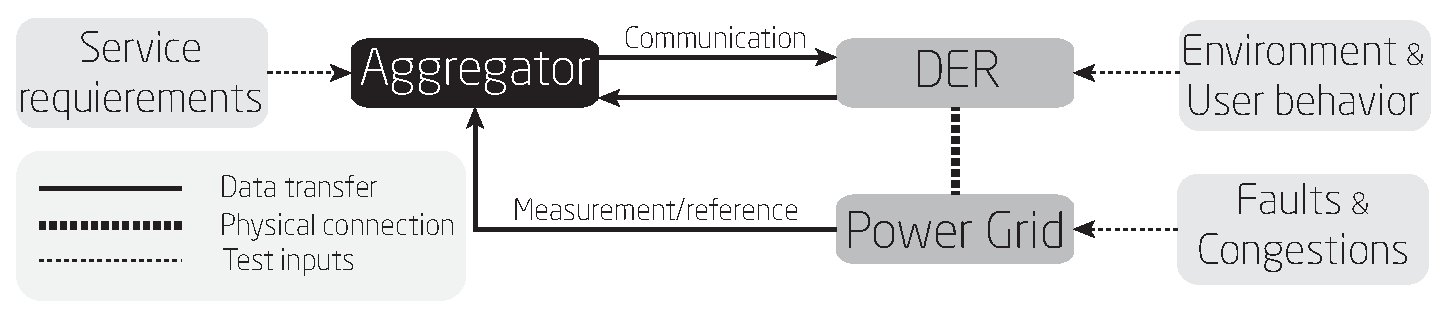
\includegraphics[width=\columnwidth]{graphics/pscc2016/test_setup.eps}
\caption{Schematic test setup where the test subject, the aggregator, is treated as a black box.}
\label{fig:test_setup}
\end{figure}

\subsection{Service Requirements - Test Metrics}\label{sec:servreqmet}

In order to measure how the disturbances affect service delivery, a set of service performance metrics must be established. The main purpose of the current tests is to verify communication, responsiveness to frequency changes and tracking of a reference or AGC\footnote{Automatic Generation Control, see e.g.\cite{entso1operational}.} signal. Coupling this with the performance requirements defined by the TSOs (e.g. \cite{energinet2012ancillary,ipower2013development}), the expected behavior of the considered services was analyzed (Table~\ref{tab:servmet}), and a set of requirement metrics were defined:
\begin{itemize}
\item Time responsiveness, i.e. how fast can the service be delivered from the moment the reference or measurement signal changes.
\item Grid responsiveness, i.e. how well can the aggregator follow changes in the grid state (marked with $\star$ where relevant on Tab.~\ref{tab:servmet}).
\item Response accuracy, i.e. how good is the aggregator in providing the full volume that is requested.
\end{itemize}


\begin{table}[!t]%% increase table row spacing, adjust to taste
\renewcommand{\arraystretch}{1.30}
% if using array.sty, it might be a good idea to tweak the value of
% \extrarowheight as needed to properly center the text within the cells
\caption{System services and their behavior}
\label{tab:servmet}
\centering
% Some packages, such as MDW tools, offer better commands for making tables
% than the plain LaTeX2e tabular which is used here.
\begin{tabularx}{\columnwidth}{p{1.0cm} X X}
\toprule
System Operator& Service name & Service behavior\\
\midrule
TSO & Frequency containment reserve (FCR) & autonomous response to frequency deviations ($\star$) \\
TSO & Frequency restoration reserve (FRR) & tracking of the AGC-signal\\
DSO & Congestion management         & reference tracking \\
    &                               & respecting a maximum feeder/transformer limit ($\star$) \\
    &                               & demand response \\
    &                               & grid state responsiveness ($\star$)\\
\bottomrule
\end{tabularx}
\end{table}

These three metrics will constitute the measure with which an aggregator will be deemed to perform according to service requirements, and the tests must excite the aggregator such that it is possible to determine through the value of these metrics the performance of the aggregator. It must be pointed out that the grid responsiveness metric is only applicable to the evaluation of aggregators providing services that rely on direct measurement of the grid, e.g. FCR.

When system operators define the acceptable values of the service requirement metrics, the values should have a statistical component. An example could be that the time responsiveness of a service provision should in average of 5 seconds, with a variance of $\pm$ 1 second. The actual indices used for the proposed metrics are discussed in Sec.\ref{sec:evaluation}.

\subsection{Aggregator Validation Procedure}\label{sec:alignment}
The procedure for aggregator validation applies statistical principles for the evaluation of the aggregator performance. It consists of the following steps:
\begin{enumerate}
	\item The general composition of the aggregator is established through documentation, and the service the aggregator is to be validated for is selected. %The aggregator informs of the general composition of its portfolio, as well as the service it wants to be validated for.
	\item The testing entity identifies the appropriate service requirements for the selected service.
	\item The testing entity identifies the expected normal operation of the aggregator based upon the service definition.
	\item The testing entity defines the operation scenarios that the aggregator is expected to perform under. %The scenarios must define the statistical properties, e.g. mean and variance, for the stochastic disturbances affecting the aggregator performance.
	\item The tests are carried out on the aggregator.
	\item The aggregator performance is evaluated.
\end{enumerate}

From the services analysed in this work, the tests are divided into two categories depending on their excitation signal:
\begin{itemize}
\item step response (like those for FCR),
\item continuous reference tracking (like those for FRR).
\end{itemize}

The validation tests will use one of these excitation signals under a different set of circumstances defined in the operation scenarios. Sufficient sampling of the aggregator response to the excitation signal is important in order to ensure that the mean and variance of the performance metrics give a realistic impression of the aggregator performance under deployment.%Thus, we formulate the following heuristic for the alignment of service requirements and tests: if a service
%The tests will evaluate the sensitivity of the aggregator to changes in the portfolio, and issues with the communication.


%\hl{The test procedure should be described. 2 diagrams are needed: 1st. shows the aggregator under normal operation (physical connection and the ICT connection), with relevant inputs and outputs of the aggregator. 2nd is the test process, where at each stage inputs are added/modified.}

% At the same time, based upon these two inputs, the overall service delivery is verified and evaluated, which is reflected in the bottom box of Figure~\ref{fig:framework}. \hl{Generally, I think we're still talking too much about the overall process and not about what the paper claims it's focusing on ("[...] the alignment of service requirements with the testing [...]"). On the latter we're not specific enough wrt what kind of result the reader can expect.}

%An aggregator infrastructure and control process is usually complex and therefore interactions of an aggregator may be tested separately. Depending on the metrics by which the relations are measured (Table~\ref{tab:metrics}), it is possible to test certain components through simulation or co-simulation, while other interactions require hardware-in-the-loop tests. This paper will propose a method for identifying the relationships between metric types and the tests necessary  for validating the measured function. The method will then be applied to several existing aggregator architectures as a proof of concept.

\subsection{Evaluation of Test Results}\label{sec:evaluation}
The service requirement metrics (Sec.~\ref{sec:servreqmet}) define the measure upon which the aggregator is evaluated. Different options exist that can be used to measure these metrics. One option is the aggregator performance index \cite{bondy2014performance}, which measures the error in service delivery for the services delivered to the system operators and the serviced delivered to the owners of the DERs. This metric captures both time responsiveness and response accuracy into a single value. A large set of performance indices exist within the field of control performance assessment, these can be utilised for the proposed validation method, see e.g. \cite{jelali2006overview}.

Given the stochastic nature of the tests, the indices will also be stochastic. The value of the performance indices is estimated at each iteration of the test, which means that the final value of the performance index reflects the stochasticity of the disturbances. For example, if the disturbances defined in the operation scenarios are Gaussian, the performance index will also have a mean and variance. These values need to be compared to those values defined in the service requirements. It will be the choice of the system operators what the service requirements should be, taking into consideration their risk adversity. Requiring a small variance on the performance indices minimizes the risk of not getting a full service delivery, but might also lead to more expensive services.


%\input{content/assumptions.tex}
\section{Case Study of the Validation Procedure }\label{sec:casestudy}

In this section we apply the concepts outlined in Sec.~\ref{sec:metrics} on a simplified example of the validation procedure on an aggregator architecture similar to the one presented in \cite{thavlov2013aggregation}. While the design of these operating scenarios is outside the scope of this paper, some overall assumptions have been made. The sample aggregator name is  DTU-FlexServices, and it wants to sell ancillary services to the TSO called RisøGrid. The validation tests are carried out by the independent company AggTesters. The rest of this section presents the reference scenario, the example of the aggregator test and the evaluation process. 

\subsection{Aggregator Framework \& Portfolio}
The objective of the DTU-FlexServices is to allocate a given amount of power, provided as a setpoint by the TSO, over a controllable portfolio of 100 resistive heating systems, each providing space heating to a detached household. The objective is subject to constraints on nominal power of the heating systems and indoor comfort, which is implemented as a tolerable band in which the temperature is allowed to vary given by the interval $\left[T_{min},T_{max}\right]$. It is assumed that feedback on measured indoor temperature is available to the aggregator, such that the aggregator in real-time can assess the available capacity of the controlled heating system and ensure that indoor temperature constraints are not being violated during operation. Fig. \ref{fig:flow_diagram} presents the flow of data in the aggregator simulation framework. 
\begin{figure}[!t]
\centering
\includegraphics[width=\columnwidth]{graphics/pscc2016/flowchart.eps}
\caption{Flow diagram of the aggregator algorithm.}
\label{fig:flow_diagram}
\end{figure}
The aggregator uses a simple auto-regressive model with exogenous inputs (ARX) to assess the future available capacity of each individual households. The ARX model is given by,
\begin{equation}\label{eq:capacity}
  T_{i+1} - a\cdot T_i = b \cdot T_{a,i} + c \cdot \Phi_{s,i} + \boldsymbol{d}^T \boldsymbol{\Phi}_{h,i:i-\tau_{lag}}
\end{equation} 
where $T_i$ is the measured indoor temperature of the household at time step $i$, $T_a$ is the outdoor temperature, $\Phi_s$ is the solar irradiance and $\boldsymbol{\Phi}_{h,i:i-\tau_{lag}}$ is a vector with the most recent observed power consumptions, i.e. $\left[\Phi_{h,i},\Phi_{h,i-1} \cdots \Phi_{h,i-\tau_{lag}}\right]$. The lag parameter of the heat input, $\tau_{lag}\in\mathbb{N}_0$, is used to account for the potential time-lag that might exists between when heating is applied and when it is observed in the indoor temperature. $a$, $b$, $c\in\mathbb{R}$, and $\boldsymbol{d}\in\mathbb{R}^{\tau_{lag}+1}$ are the unknown parameters of the ARX model, which are found using prior data for power consumption of the heating system. For simplicity $\tau\equiv 0$ is assumed in the following. 

Each individual resistive heating system is assumed to be able to dispatch a continuous amount of power in the interval $\left[P_{min}, P_{max}\right]$, given by the nominal power of the heating system. Naturally, this is an approximation since resistive heating systems, in general, will only be able to dispatch power in discrete steps due the composition of resistive loads. However, considering a portfolio of many entities and following the law of large numbers, these discrete steps should level out and the assumption hold. 

To allocate the amount of power over the portfolio of resistive heating system, following unit commitment problem is formulated,
\begin{align}\label{eq:agg_dispatch}
  & \min\;\left|\; \sum_{j=1}^N \left(\Phi_{h,i,j}\right) - S_i \;\right|\; + \; \sum^{N}_{j=1}\Phi_{h,i,j}\mbox{W}\left(T_{i+1,j}\right)	\\[5mm]\nonumber
  & \mbox{s.t.} \quad P_{min,j} \leq \Phi_{h,i,j} \leq P_{max,j}  
\end{align}
where the decision variable  $\Phi_{h,i,j}\in\mathbb{R}$ is the amount of power being allocated to household $j$ at time step $i$, $N$ is the number of households in the portfolio, $S_i$ is the setpoint given to the aggregator and $\mbox{W}\left(T_{i+1,j}\right)$ is a weight function of the predicted indoor temperature found from Equation \eqref{eq:capacity}. The weight function should be constructed such that $\mbox{W}\left(\cdot\right)<-1$ for $T_{i+1,j} < T_{min}$, thus making the last term dominate the cost function and force the allocated power up for household $j$. Likewise, $\mbox{W}\left(\cdot\right)>1$ for $T_{i+1,j} > T_{max}$, thus forcing the power down. Following linear weight-function is proposed,
\begin{equation}\label{eq:weight_fct}
  \mbox{W}\left(T_{i+1,j}\right) = \frac{2\left(T_{i+1,j}-T_{min,j} \right)}{T_{max,j} - T_{min,j}}-1 
\end{equation}
The simulation model of the individual households is implemented as a stochastic linear state space model in discrete time, which is     given by
\begin{align}\label{eq:simulation_model}
  \boldsymbol{T}_{i+1} &= \boldsymbol{A}\boldsymbol{T}_i + \boldsymbol{B}\boldsymbol{U} + \boldsymbol{\sigma}_i \\\nonumber
  T_i &= \boldsymbol{C}\boldsymbol{T} + e_i
\end{align}
where $T_i\in\mathbb{R}$ is the locally measured indoor temperature which is assumed to be forwarded to the aggregator, $\boldsymbol{T}_i\in\mathbb{R}^n$ is the state vector and $\boldsymbol{U}\in\mathbb{R}^m$ is the input vector. $\boldsymbol{A}\in\mathbb{R}^{n\times n}$, $\boldsymbol{B}\in\mathbb{R}^{n\times m}$ and $\boldsymbol{C}\in\mathbb{R}^{1\times m}$ are the system, input and output matrix, respectively. To account for unrecognized input and approximations, process noise, $\boldsymbol{\sigma}_i\in\mathbb{R}^n$, is added to the system equation, \eqref{eq:simulation_model}. In the following, $\boldsymbol{\sigma}$ is assumed to be a Gaussian white noise process. Furthermore, $n\equiv1$ is assumed, i.e. only one temperature state is being simulated in the households; hence, since a Gaussian white noise process is fully characterized by its variance, the process noise is fully described by the variance $\sigma\in\mathbb{R}$.% Naturally, a single state would not be sufficient for thermally heavy households with multiple heat reservoirs, e.g. households with floor heating.

The aggregator framework and simulation models, simulating the considered scenario, have been implemented in \textsc{matlab} and is presented in full detail in \cite{thavlov2013aggregation}. It is important to note that the aggregator is described in this section for the purpose of the paper, but this description is contained within the conceptual black box described in Sec.~\ref{subsec:assumptions}, and the testing entity only has access to the general composition of the aggregator portfolio.

\subsection{Service Requirements, Normal Operation and Operation Scenario}\label{subsec:scenario}
The DTU-FlexServices aggregator wants to participate in the ancillary service markets with a FRR up-regulation service with a volume of 250 kW. 
Since it is the first time DTU-FlexServices participates in the market for this service, RisøGrid requires DTU-FlexServices to go through the validation process. Following the steps outlined in Sec.~\ref{sec:alignment}, the validation process consists of the following steps:
\begin{enumerate}
\item DTU-FlexServices presents the documentation for its portfolio.
\item RisøGrid sets the test service requirements as:
    \begin{itemize}
        \item Response accuracy:  $E[RMS] \leq 60\,kW$
        \item The response durations: $\tau = 1\,h$
    \end{itemize}
\item AggTesters identifies the normal operation scenario as:
    \begin{itemize}
        \item One source of uncertainty is the availability of the portfolio, which is a uniform distribution between 70\% and 100\%. This also accounts for minor changes in the portfolio size.
        \item A second source of uncertainty is in the disturbances induced by unrecognized user behavior and inaccurate weather forecast in the house simulation model. This uncertainty is described by $\sigma$ in Eq.~\eqref{eq:simulation_model}.
    \end{itemize}
\end{enumerate}

\subsection{Aggregator test}
To test for different combinations of the two sources of uncertainties, a series of simulations are carried out with permutations of the two. Assuming the availability to be uniformly distributed, the tests are carried out in discrete steeps across the 70\% -- 100\% spectrum of availability. Likewise, the variance of the noise process is tested in discrete steps in the 0.00 -- 0.30 domain. Fig.~\ref{fig:test100} and Fig.~\ref{fig:test70} present the outcome of two different simulations for 100\% and 70\% availability, respectively, and $\sigma=0.10$. Each permutation of the two noise sources is simulated 100 times.
\begin{figure}[!t]
%\centerline{
\centering
\subfloat[Response accuracy]{\includegraphics[width=0.85\columnwidth]{graphics/pscc2016/agg_power_ctrl_100SH_0STATIC_05PCT_REDUCTION.eps}%
\label{fig:ref100}}
%\vfill
\\
\subfloat[House Temperatures]{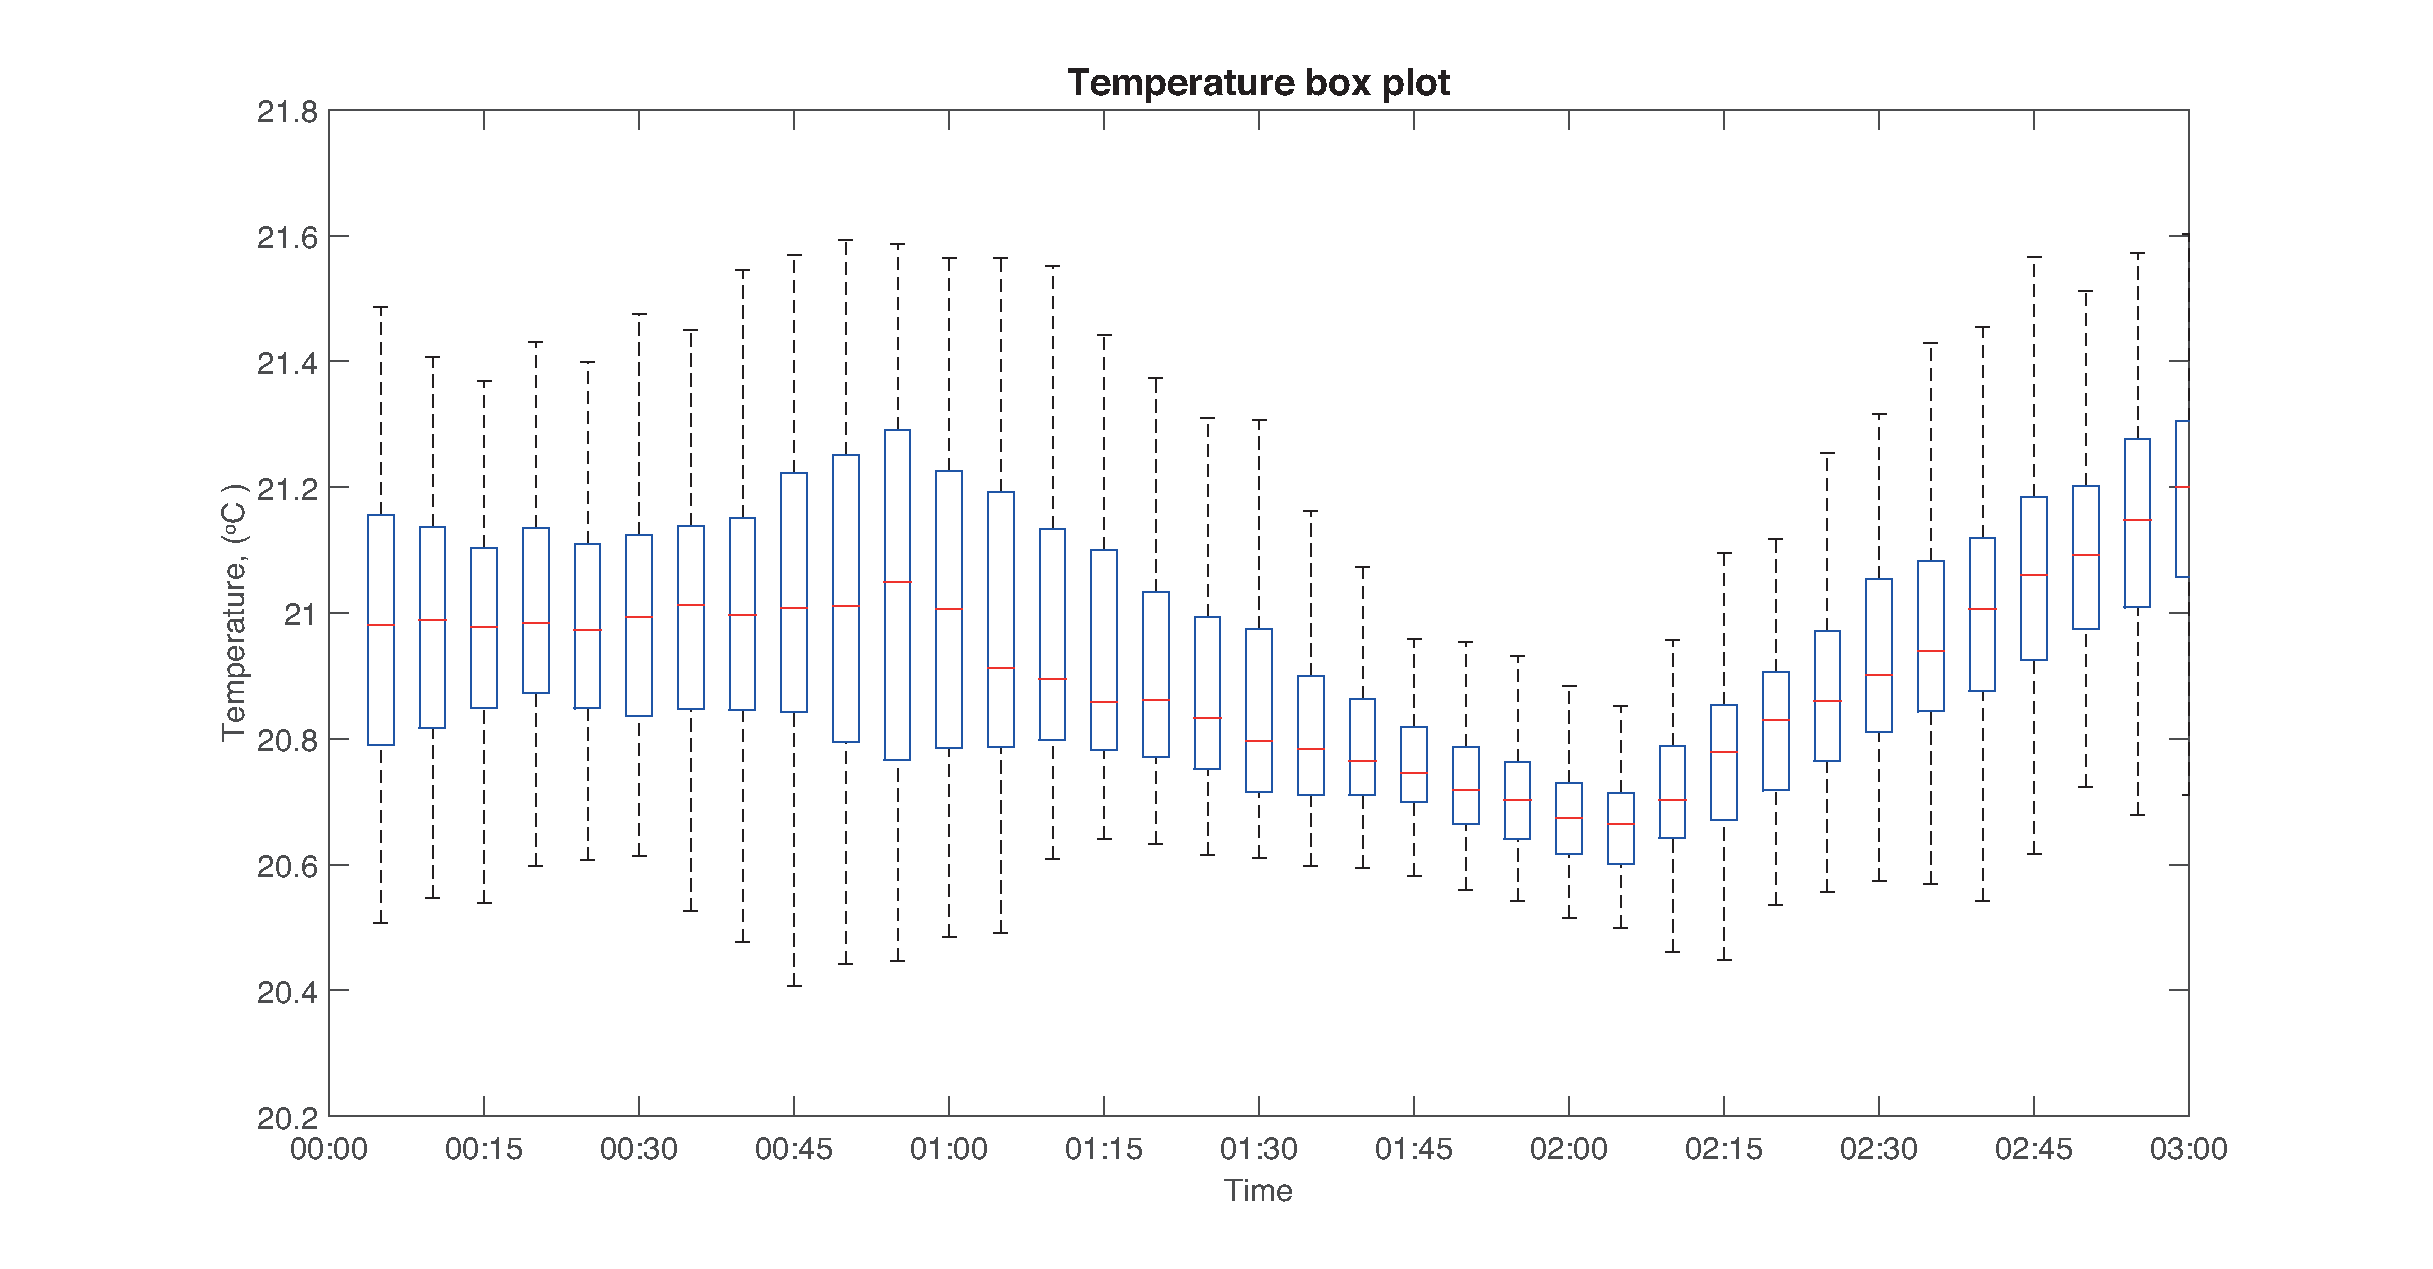
\includegraphics[width=\columnwidth]{graphics/pscc2016/agg_box_plot_100SH_0STATIC_05PCT_REDUCTION.eps}%
\label{fig:temp100}}%}
\caption{Simulation results of the 100\% availability test for the whole portfolio.}
\label{fig:test100}
\end{figure}

\begin{figure}[!t]
%\centerline{
\centering
\subfloat[Response accuracy]{\includegraphics[width=0.85\columnwidth]{graphics/pscc2016/agg_power_ctrl_70SH_30STATIC_05PCT_REDUCTION.eps}%
\label{fig:ref70}}
%\vfill
\\
\subfloat[House Temperatures]{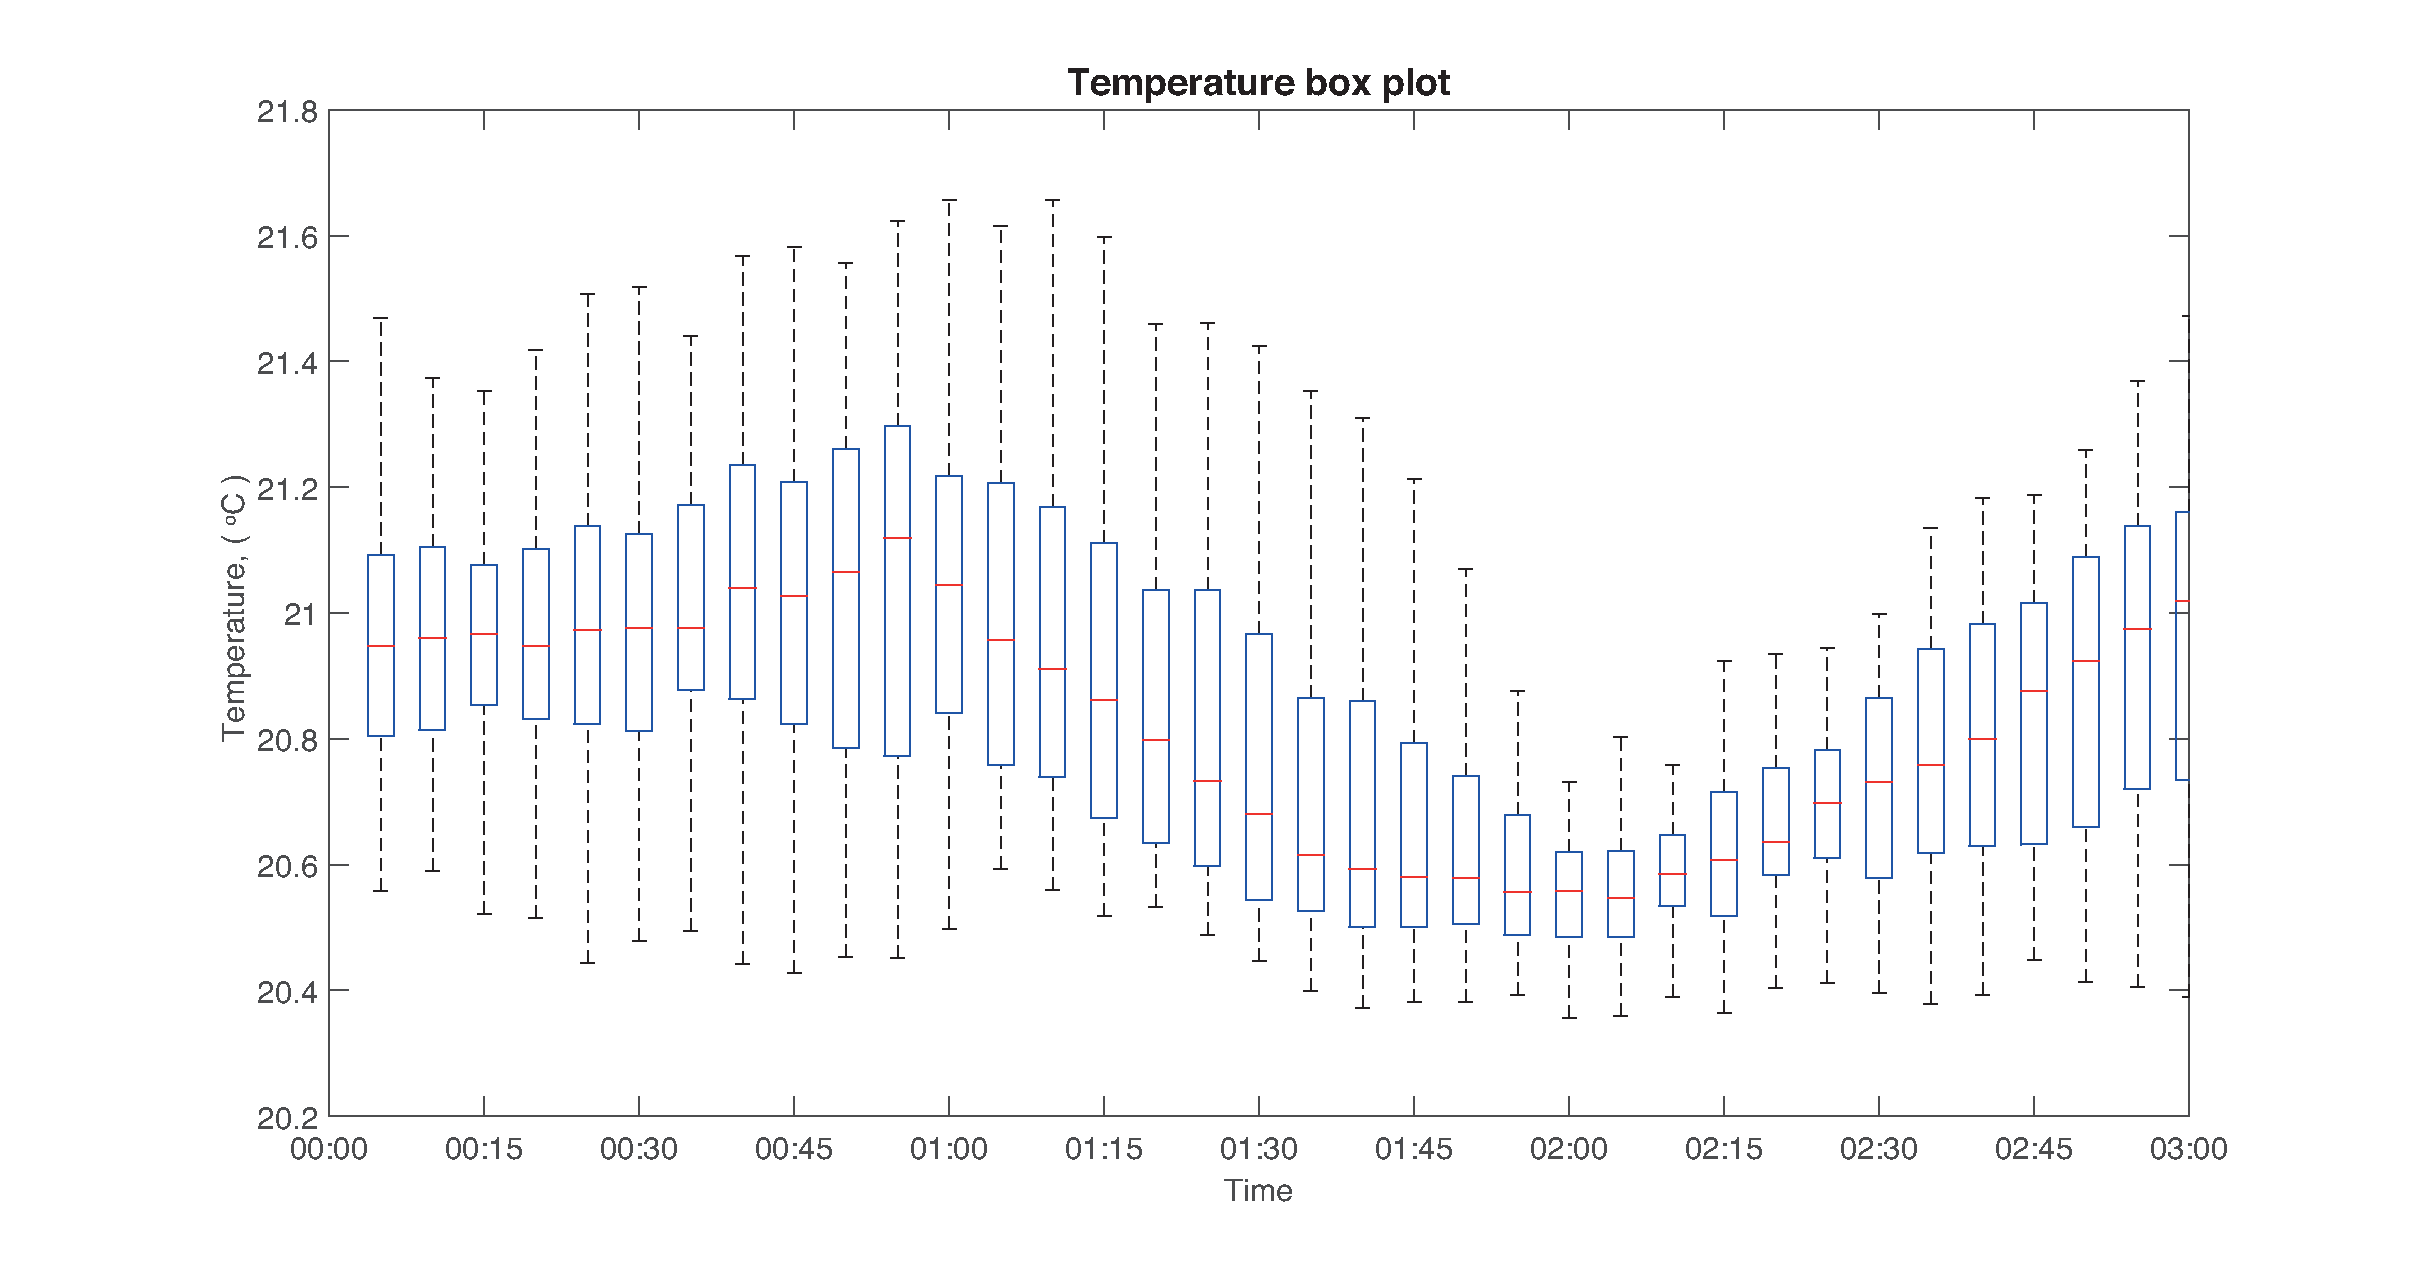
\includegraphics[width=\columnwidth]{graphics/pscc2016/agg_box_plot_70SH_30STATIC_05PCT_REDUCTION.eps}%
\label{fig:temp70}}%}
\caption{Simulation results of the 70\% availability test for the whole portfolio}
\label{fig:test70}
\end{figure}

The response accuracy of DTU-FlexServices and the average temperature of its portfolio can be seen in Fig.~\ref{fig:ref100} and Fig.~\ref{fig:ref70}. The distribution of the house temperatures can be seen in Fig.~\ref{fig:temp100} and Fig.~\ref{fig:temp70}, and it is clear that as the availability of the houses decreases, the flexibility for up-regulation is being saturated faster and the DTU-FlexServices is unable to track the FRR reference signal.

Having carried out the necessary test, RisøGrid proceeds to evaluate the results of the tests.

\subsection{Evaluation of test results}
Since the case study looks at simplified setup, and the example does not take the time responsiveness metric into account, it does not make sense to use the aggregator performance metric mentioned in Sec.~\ref{sec:evaluation}. In Sec~\ref{subsec:scenario}, the root mean square (RMS) error is chosen to measure the response accuracy metric: 
\begin{equation}
  \eta_{RMS} = \sqrt{\frac{1}{M}\sum_{i=1}^M\left(\sum_{j=1}^N\left(\Phi_{h,i,j}\right) - S_i\right)^2}
\end{equation}
where $\left[1,M\right]$ are the iterations where the aggregator has been activated. The results of the test are presented in Table~\ref{tab:results}, where it can be seen that $E[\eta_{RMS}]<60 \, kW$. Therefore the DTU-FlexServices is certified to provide FRR up-regulation service to RisøGrid.
\begingroup
\setlength{\tabcolsep}{4pt}%
\begin{table}[!t]%% increase table row spacing, adjust to taste
\renewcommand{\arraystretch}{0.9}
% if using array.sty, it might be a good idea to tweak the value of
% \extrarowheight as needed to properly center the text within the cells
\caption{Performance of DTU-FlexServices}
\label{tab:results}
\centering
% Some packages, such as MDW tools, offer better commands for making tables
% than the plain LaTeX2e tabular which is used here.
\begin{tabular}{clcccccccc}
\toprule
        & & \multicolumn{7}{c}{Process noise, $\sigma$}                   & Avg. \\
        & & 0.00   & 0.05   & 0.10   & 0.15   & 0.20   & 0.25    & 0.30   &         \\ 
\midrule
\multirow{7}{*}{\rotatebox[origin=c]{90}{Availability}} 
& 100\%   & 0.00   & 0.00   & 0.04   & 9.25   & 31.20  & 48.84   & 98.32  & 26.81   \\
& 95\%    & 0.03   & 0.00   & 1.51   & 19.19  & 37.97  & 66.56   & 102.05 & 32.47   \\
& 90\%    & 1.40   & 0.04   & 14.36  & 30.78  & 58.74  & 73.38   & 98.24  & 39.56   \\
& 85\%    & 1.10   & 35.23  & 4.06   & 45.28  & 83.06  & 83.40   & 115.11 & 52.46   \\
& 80\%    & 13.88  & 29.25  & 12.94  & 65.93  & 72.31  & 94.50   & 135.85 & 60.67   \\
& 75\%    & 54.28  & 40.74  & 39.91  & 75.22  & 86.14  & 114.13  & 135.76 & 78.03   \\
& 70\%    & 45.63  & 90.90  & 85.41  & 99.02  & 93.68  & 123.82  & 142.64 & 97.30   \\
\midrule
Avg. & & 16.62  & 28.02  & 22.60  & 49.24  & 66.16  & 86.38   & 118.28 & 55.33   \\
\bottomrule
\end{tabular}
\end{table}
\endgroup
%\begin{figure}[!t]
%\centering
%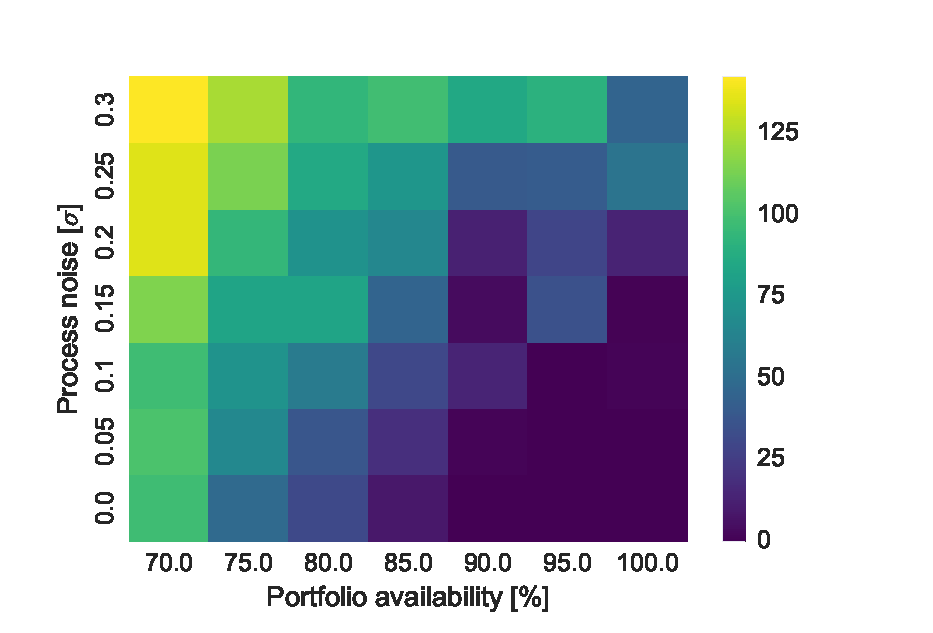
\includegraphics[width=\columnwidth]{figures/heatmap.eps}
%\caption{The RMS value over the test space. It can be seen that it is more important to have certainty in the portfolio availability than in the process noise.}
%\label{fig:colormap}
%\end{figure}

%\section{Quality Metrics}

What aspects of the aggregator influence in the performance metrics?

Internal vs. external metrics: external can be used for monitoring, internal can only manipulated in test environment.

Are there more metrics than in the table? E.g. robustness toward grid faults

\begin{table}[!t]%% increase table row spacing, adjust to taste
\renewcommand{\arraystretch}{1.3}
% if using array.sty, it might be a good idea to tweak the value of
% \extrarowheight as needed to properly center the text within the cells
\caption{System interactions can be evaluated with generalized metrics}
\label{tab:metrics}
\centering
% Some packages, such as MDW tools, offer better commands for making tables
% than the plain LaTeX2e tabular which is used here.
\begin{tabular}{ll}
\toprule
System interaction & metrics\\
\midrule
Aggregator - power system & responsiveness w.r.t. grid conditions\\
\\
Aggregator - DER portfolio & responsiveness w.r.t. time\\
 & robustness w.r.t. forecast errors\\
 \\
Aggregator -  ICT infrastructure & robustness w.r.t. communication faults\\
\bottomrule
\end{tabular}
\end{table}

\begin{table}[!t]
\renewcommand{\arraystretch}{1.3}
\caption{The quality metrics can be separated into two categories.}
\label{tab:metricsclass}
\centering
\begin{tabular}{ll}
\toprule
External metrics & Internal metrics\\
\midrule
responsiveness w.r.t. grid &robustness w.r.t. forecast errors\\
responsiveness w.r.t. time & robustness w.r.t. communication errors\\
& robustness w.r.t. grid errors\\
\bottomrule
\end{tabular}
\end{table}
\section{Discussion}
Specific terminology has been introduced to describe the proposed method. This terminology can be mapped to that of the field of \emph{Design of Experiments}, e.g. \emph{definition of service requirements} maps to \emph{definition of inner-noise factor} and \emph{definition of test inputs} maps to \emph{definition of outer-noise factors}. Specifically, the method resembles \emph{fractional factorial methods for off-line quality control}, see e.g.\cite{oehlert2010first}. In the case study presented in Sec.~\ref{sec:casestudy}, the inner factor, or controllable variable, is kept at a single level, i.e. the same activation signal is sent to the aggregator for each run of the experiment. The two outer factors, or noise variables, were varied over a distribution dictated by the operational scenario, i.e. the availability of the portfolio was varied on seven levels and, likewise, the process noise in the house simulation models was varied on seven levels. An important contribution of this work is applying this kind of formal test procedures to the problem of aggregator validation. The field of Design of Experiments is broad, and a further revision on the topic may yield a better method proposals than the one proposed here.

In this paper we focus only on the two  uncertainty sources mentioned above, therefore the test for time responsiveness, i.e. delay in the communications systems between the aggregator and a DER is not considered. This means that the test design presented in the case study is a simplified version of what an actual aggregator validation test would require. Future research must identify the relevant variables that need to be tested under the relevant operation scenarios. 

In comparison with the traditional test method, this validation procedure must capture the capabilities of a much more complex system, and therefore relies in part on simulations. As presented in \cite{steinbrink2015challenges}, the error between the used models and reality must be quantified and taken into account for the final aggregator certification. Each block in the simulation must use validated models or software. This applies to the communication systems, the grid models and the DER models. The test architecture, e.g. the one presented in \cite{buscher2015towards}, which validates the aggregators must also be validated.

There are still several open issues that need to be investigated with regards to aggregator validation. For example, the definition of the operation scenarios was only briefly discussed, and heuristics must be developed in order to define scenarios that are effective when testing aggregators.

Aggregator validation must be an ongoing process, that should be carried out periodically or whenever the aggregator portfolio or architecture changes significantly. Furthermore, aggregators are expected to participate in different electricity markets. Due to these reasons, along with the complexity of designing appropriate simulations, we believe that the task of validating aggregators should not carried out by the system operators, but by an independent third party. 
\section{Conclusion and Future Work}
This work presents an initial approach to establishing a methodology for designing aggregator validation tests. This method differs from the traditional generator certification tests in that it must be carried out in simulations, so that the stochasticity of the real world disturbances affecting the aggregator can be taken into account. A drawback of this method is that it relies on the accuracy and complexity of the simulation models. This means that the components of the validation tests must be validated against reality. The test method was shown through a simplified case study on an existing aggregator. While the example shows a fictive TSO applying the test to a fictive aggregator, there is the possibility that validation of aggregators in the future will be carried out by third party test companies. 

There are still several open issues that need to be investigated with regards to aggregator validation. For example, the definition of the operation scenarios was only briefly discussed, and heuristics must be developed in order to define scenarios that are effective when testing aggregators.

An important step for the development of the validation method is the implementation of a complete test architecture with validated component models. With such a simulation framework, with realistic communication and DER models, communication delays can be implemented in order to test aggregators for time responsiveness. 

Finally, the method should be expanded to cover other ancillary services, such as voltage regulation.

We consider the work presented here an important element of enabling aggregators in the smart grid, thus enabling consumption to actively participate in the secure operation of the power system. This will help the integration of renewable energy sources into the power system.



%!TEX root = ../Thesis.tex
\chapter{Method for Ancillary Service Modeling and Performance Assessment}
\label{app:segan}

\textbf{Authors:}\\
Daniel Esteban Morales Bondy\\
Anders Thavlov\\
Janus Bundsgaard Mosb{\ae}k Tougaard

\noindent
\textbf{Submitted to:}\\
Journal on Sustainable Energy, Grids and Networks 

\noindent
\textbf{Abstract:}\\

Traditional sources for ancillary services are diminishing as intermittent distributed renewable energy sources supplant traditional fossil-fueled generation units. Aggregation of large quantities of consumption units is expected to be a new source of energy services, including power system ancillary services.
While the performance capabilities of fossil-fueled generation units is well understood, the performance assessment of aggregation algorithms needs to be analysed. Furthermore, ancillary services need to be modeled such that aggregated services can be verified.
This paper presents a novel modeling method for ancillary services. The service models are useful for assessing the performance of aggregators. The paper also presents performance and verification indices for aggregator service provision.
The use of the modeling method and the indices are exemplified in three case studies.
These concepts are critical if aggregators are to help ensure the security of the power grid in a future with high amount of intermittent power generation. 


\noindent
\textbf{Keywords:}\\
Ancillary Service Modeling; Performance Assessment; Aggregator; Demand Side Management

\section{Introduction}
The power industry is experiencing a significant shift away from being based on fossil fuels towards more generation from Renewable Energy Sources (RES). The tendency is that a substantial amount of the RES are distributed energy resources (DER), which alters the traditional top-down approach in the sector, where a relatively few number of large power plants provides electric power and ancillary services. Furthermore, there is a growing electrification in the energy sector with heating and transportation being the largest energy consumers. The non-dispatchable and stochastic nature of RES and the increasing electrification of consumption, call for new sources of ancillary services. One of these sources will be demand response (DR) from small-scale entities, e.g. private consumers, whose flexibility in consumption will be harnessed by aggregators \cite{pudjianto2007virtual}. With the introduction of aggregators, as providers of ancillary services, a versatile method for ancillary service modeling and performance assessment is needed.

Currently, performance assessment of units providing services to the grid operators is done as a pass/non-pass evaluation based upon the minimum service requirements \cite{EnerginetAncillary}. While performance criteria have been formulated for specific services, e.g. load frequency control \cite{gross2001analysis} or primary frequency control \cite{eto2010use}, these focus on the overall performance of the reserves seen from a grid perspective, i.e. the criteria do not evaluate the individual performance of each service-providing unit. Furthermore, until now, the performance assessment of aggregators in academia has been ad-hoc to specific aggregator implementation, e.g. \cite{vrettos2015integrating}, or the evaluation focus has been on computational or financial performance, e.g. \cite{su2012performance,rahnama2014evaluation}. Similarly, a platform for simulation of aggregation strategy is proposed in \cite{dittawit2014demand}, but the focus is on the simulation tool, which focuses only on the demand side, and not on the process of validation. None have taken a systematic approach to generally evaluating the performance of the aggregators in terms of the contractual requirements of service delivery. 

This paper presents a novel method for modeling a generic set of active power ancillary services as well as distribution system congestion management services. Furthermore, it is shown how these models can be used for performance assessment of aggregators. The article refines the concept of a service performance assessment index and Quality of Service, both treated in previous work, and further introduces a novel way of assessing the non-delivery of a service. The non-delivery assessment is proposed for verification of the aggregator service delivery.

The rest of the article is organized as follows: background concepts for the work are presented in Sec.~\ref{sec:SEGANbackground}, the modeling method is presented in Sec.~\ref{sec:SEGANmethodology} and the service performance assessment and verification indices are presented in Sec.~\ref{sec:SEGANperformance}. The use of the service modeling and indices are shown through three case studies in Sec.~\ref{sec:SEGANcasestudies} and concluding remarks are presented in Sec.~\ref{sec:SEGANconclusion}.


\section{Background}\label{sec:SEGANbackground}
In this section, the terminology and concepts utilized throughout the paper are defined. The study is based on the Danish market for ancillary services, but the method presented here can be transferred to other markets.  

\subsection{Ancillary services}
Ancillary services are utilized by transmission system operators (TSOs) to ensure a adequate and secure operation of the power system. There is a variety of services targeting different aspects of the power system operation. This work will focus solely on active power control, but the method presented here can be translated into other types of services, e.g. control of reactive power for voltage control. Currently, frequency containment reserve (primary reserve) and frequency restoration reserve (secondary reserves) \cite{entso1operational} are widely utilized by TSOs to ensure frequency stability. In the future, such services are expected to be delivered by aggregators \cite{pudjianto2007virtual,vrettos2015frequency}. Furthermore, with the introduction of aggregators, new possibilities arise for solving problems at distribution system level, e.g. congestion issues, leading to new flexibility services being defined for distribution system operators (DSOs), as presented in \cite{ding2013development}. %, which can also be delivered by aggregators. This work will present an examle of each type of service.  
%defines seven DSO-flexibility services, which can be traded through a flexibility clearing house (FLECH). Five of these concern active power regulations and two voltage management services. 

\subsection{Flexible distributed energy resources}\label{sec:DERs}
With an increased electrification of the energy system due to the introduction of electric vehicles (EVs), heat pumps and local generation, DERs are expected to deliver an increasing amount of ancillary services in the future power grid. The DERs that can be utilized for ancillary services are those which can provide flexibility in consumption or generation without significantly impacting their primary energy service, e.g. battery state of charge and indoor temperature comfort \cite{costanzo2013coordination,halvgaard2012economic}.

The incentive for a DER owner of contracting an aggregator to manage his flexibility will likely be economical by receiving a payment for his availability. However, the incentive could also be non-economical; for example, the aggregator could offer actual services to the DER owner, e.g. efficient operation of heat pumps by live monitoring of the coefficient of performance or provision of a web interface for indoor climate control, which allows the DER owner to control the indoor temperature in his home. Another option could be that the aggregator controls a cluster of units owned by a single actor, e.g. the aggregator acts as a fleet operator for the optimal charging of a pool of EVs owned by single entity. Similarly, it could also be in control of the heating of an office building, where the overall temperature of all offices should respect certain comfort bounds. In the following, such services will be referred to as asset management services (AMS). % \bondynote{Anders, you had a few ideas here didn't you?}

%Examples of relevant DERs are electrical vehicles, which can charge dynamically and achieve peak-shaving at the point of connection, while still respecting some overall performance requirements like a specific state of charge in the morning \cite{costanzo2013coordination}. An electrical heat pump for residential heating can in some situations during winter shift its consumption more than half a day to achieve an economic benefit for the owner as described in \cite{halvgaard2012economic}. Residential refrigerators can significantly reduce the frequency nadir by providing a fast reacting primary reserve, while secondary reserves can come from electric water heaters and heating, ventilation and air conditioning systems of commercial buildings as described in \cite{vrettos2015frequency}.
%\subsection{Congestion management and DSO services}
%It is anticipated that the DSOs will start to utilize flexibility in the future (ref).
%
%Different grid tariffs are alternatives to power system services (NEAS ref).

\subsection{Players/roles in the market for ancillary services}
In Denmark, ancillary services are acquired by the TSO through an open market, where approved participants can bid their reserves. The bid size varies with the service, but generally the minimum bid size is larger than what most DERs can provide by themselves \cite{EnerginetAncillary}. Such market requirement further increases the need for aggregators, which can pool large amounts of DERs and represent them in the market as a single legal entity. Furthermore, most DER owners will likely not have the time, interest or knowledge to control their consumption 24 hours a day. 
%Because of this, a party called an Aggregator is needed, who pools a larger body of DER units and are responsible for the operation of these units. 
The aggregator can deliver TSO and DSO services as well as flexibility services for balance responsible parties (BRPs). BRPs are responsible for the balance of power production or consumption within their portfolio and they already trade energy in the power markets. The actors and their relationships can be seen in Fig.~\ref{fig:SEGANmarket}. Finally, in order to avoid the aggregator creating imbalances for the Balance Responsible Consumer, all aggregator-service sales must occur through the Balance Responsible Consumer. 
\begin{figure}
  \centering
  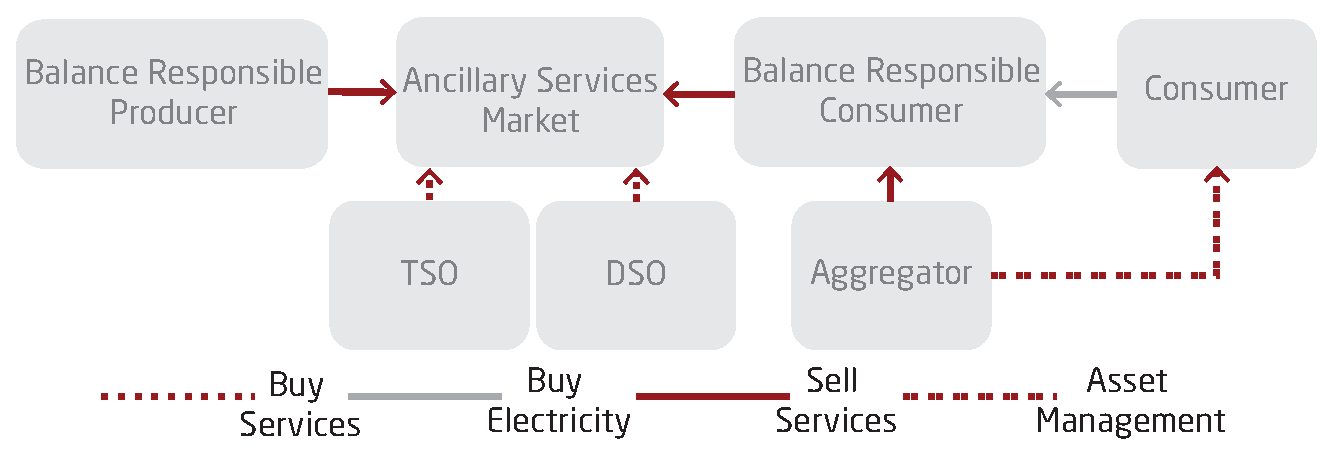
\includegraphics[width=\columnwidth]{SEGAN/market_future3.eps}
  \caption{The new player in the market for ancillary services is the aggregator, which sells consumption flexibility on the ancillary service markets through the Balance Responsible Consumer. Some markets allow the aggregators to participate directly in the ancillary service markets with the condition that they coordinate with their Balance Responsible Consumer.}
  \label{fig:SEGANmarket}
\end{figure}
%The aggregator will sign contracts with the DER owners and be the responsible party for delivery of service to the TSO, DSO or BRP. Further, the aggregator will have to ensure that certain performance parameters are respected towards the DER owner \cite{ding2013development}.
%Introduction of FLECH. \newline


\section{Method for service modeling}\label{sec:SEGANmethodology}
Currently, services requirements are defined in a contract, but there is no standardized method for transforming contractual requirements into a mathematical model (requirements model) that a computer can use for verification of service delivery. This requirements model forms the base-line against which the delivered service is benchmarked. The model incorporates both the ideal and acceptable service provision. By analysis of the TSO services defined in \cite{EnerginetAncillary}, the potential DSO services defined in \cite{ding2013development} and asset management services, we have developed a method for modeling the service delivery over time. 
%The method presented in this section outlines the steps to transforming contractual requirements into a requirements model.
The method consists of the following six steps:
%form have been identified as a generic method for modeling ancillary services. The steps are exemplified by DSO services defined in  and TSO services defined in :
\begin{enumerate}
  \item Identify physical parameters defining the service.
%  \begin{itemize}
%    \item For example: Power production or consumption, measured grid frequency, time measurements. Including maximum measuring sensitivities.
%  \end{itemize}
  \item Identify the dynamic behaviors of the service related to system parameters (if any).
%  \begin{itemize}
%    \item Example: Primary frequency regulation comes with a linear behavior between grid frequency and generator set-point. Power-cap has a dynamic relationship between feeder load and the controllable load power in order to keep the total feeder load at a $P_{DSO,Ref}$ value.
%    \item PowerMax is not dynamic. The aggregator must control $\Delta P_{Agg}$ to ensure that he does not violate $P_{max,Agg}$. But the service does not require a dynamic behavior related to a system parameter like primary frequency regulation and PowerCap.
%  \end{itemize}
  \item Identify the physical size of the service and the tolerated error. % Both ideal service and minimum required service.
%  \begin{itemize}
%    \item Physical size is for example $P_{max,Agg}$ for PowerMax service or regulation bid for primary frequency regulation.
%    \item Tolerance is for example $P_{max,Agg}+P_{tolerance}$ for the PowerMax service and allowed dead-band for DK1 primary reserve.
%  \end{itemize}
  \item Identify the ideal response time of the service and acceptable response.
%  \begin{itemize}
%    \item Most contracts comes with some timing specifying how fast the service provider must act.
%    \item E.g. DK1 primary reserve must provide 50 \% of service within 15 s and 100 \% within 30 s.
%    \item The ideal service is for example an instantaneous step in power to 100 \% of set-point for DK1 primary reserve.
%  \end{itemize}
  \item Based on the dynamics, size and timing of the service, as well as the tolerated errors from points 1--4, develop a time series for ideal and acceptable service provision. The model will be a set of time series: $\mathbf{x}_{ideal}(t)$ for ideal response and $\mathbf{x}_{acc}(t)$ for acceptable response. Both time series can be a scalar or a vector, e.g. $\mathbf{x}_{acc}(t)$ can be formed by a set of upper and lower tolerance bounds or simply by an upper bound.
  %§$\mathbf{x}_{ideal}(t)$ and $\mathbf{x}_{acc}(t)$ can be a pair of values, e.g. minimum and maximum tolerance limits, for some services and may be only a single value, e.g. minimum or maximum tolerance, for others. 
  \item Identify how the service error is to be measured.
\end{enumerate}

We identify three different types of service: reference tracking, band service or a maximum/minimum cap. The error measure, $e(t) \in \mathbb{R}$, for each of the service types is defined in the following subsections. This approach was initially introduced in \cite{bondy2014performance}, and is further refined in this work. 

%The error, $e(t) \in \mathbb{R}$, in the delivery of a service can be calculated using a reference tracking, band service or a maximum/minimum cap approach. The proposed approach depends on the specific service and contract.\bondynote{These last two paragraphs can probably be merged}


\subsection*{Reference tracking}
Reference tracking error can be calculated as:
\begin{equation}\label{eq:ref_error}
e(t) = x_{meas}(t) - x_{ideal}(t).
\end{equation}
This definition will lead $e<0$ for measured values below the ideal and $e>0$ for values above the ideal. In this case $\mathbf{x}_{acc}(t)$ will be a band around $x_{ideal}(t)$, and the values of $\mathbf{x}_{acc}(t)$ do not need to be symmetric.

\subsection*{Band service}
The ideal response in a band service is defined as $ \mathbf{x}_{ideal}(t)= [x_{min}(t),x_{max}(t)]$. The error in the band service can therefore be estimated by:
\begin{equation}\label{eq:band_error}
e(t)=
\begin{cases}
x_{meas}(t) - x_{min}(t) , & x_{meas}(t) < x_{min}(t)  \\
0, & x_{min}(t) \leq x_{meas}(t) \leq x_{max}(t) \\
x_{meas}(t) - x_{max}(t), & x_{meas}(t)  > x_{max}(t).  
\end{cases}
\end{equation}
In this case, the $\mathbf{x}_{acc}(t)$ is a set of values that surrounds the band defined by $ \mathbf{x}_{ideal}(t)$, as seen in Fig.~\ref{fig:RefErr}. The values of $\mathbf{x}_{acc}(t)$ do not need to be symmetric around the band.

\subsection*{Cap service}
%Maximum/minimum cap error only counts the error when performance is above/below some ideal value. 
In cap services, error is only tracked when $x_{meas}(t)$ is either above or below a given a limit value.
Maximum cap error is calculated as shown in \eqref{eq:maxmin_cap} and minimum cap can be similarly calculated. In \eqref{eq:maxmin_cap}, $x_{max}(t)$ is the ideal maximum limit according to the service contract:

\begin{equation}\label{eq:maxmin_cap}
e(t)=
\begin{cases}
x_{meas}(t)-x_{max}(t), & x_{meas}(t) > x_{max}(t) \\
0, & x_{meas}(t) \leq x_{max}(t).
\end{cases}
\end{equation}
In the cap service, $x_{acc}(t)$ is a limit that either lies below $x_{min}(t)$ or above $x_{max}(t)$.

Having defined the method for formulating the service models, we will show how these can be used for performance assessment of services.


\section{Performance Assessment of Service Delivery}\label{sec:SEGANperformance}
The concept of performance assessment of the service delivery of aggregators was presented by one of this work's authors in \cite{bondy2014performance}, but inconsistencies and shortcomings have been found in the proposed assessment index. Based upon work presented in \cite{thavlov2015thesis}, the service performance assessment index is corrected and expanded upon here. In order to asses service performance three concepts are introduced in this section:
\begin{itemize}
\item Quality of service, which is an instantaneous measure of how well the aggregator is delivering one service within the contract constraints;
\item service performance assessment index, which describes the overall performance of the aggregator over the delivery period for the services, or subset of services, it is providing; and a
\item service verification index, which describes how much an aggregator is breaking the contractual agreements (non-delivering) of the services, or a subset of services, it provides.
\end{itemize}

Differently from the previous work, the service delivery index is split into measures of the ancillary services (AS) delivered to system operators and the AMS delivered to unit owners (see Sec.~\ref{sec:DERs}). In this way, a system operator (or a third party certification company) can use the index for certification of aggregators, for which the AMS evaluation is irrelevant. Furthermore, the service verification index is introduced, and a new way of defining the quality of service is presented.
%\athanote{We should be a bit more explicit about services delivered upwards in the system (AS) and down-wards (AMS) to the asset owner}

\subsection{Quality of Service}
Quality of service (QoS) is a measure defined in \cite{bondy2014performance}, where it is used to assess the quality of a power system service at any given time. QoS at any given time is given by:
\begin{equation}\label{eq:QoS}
QoS(t)=e(t)C_{s}(t)
\end{equation}
where \emph{e(t)} is the error in service delivery introduced in Sec.~\ref{sec:SEGANmethodology}, and $C_s(t)$ is a normalization factor that can be time varying. By definition:
\begin{itemize}
\item $QoS \geq 0$;
\item for $QoS \leq 1$ the service is considered delivered within the contractual constraints;
\item and $QoS = 0$ is a perfect service delivery.
\end{itemize}
In order to achieve these definitions, the normalization factor $C_{s}(t)$ must be calculated from $\mathbf{x}_{acc}(t)$ thus:
\begin{equation}
C_{s}(t) = 
\begin{cases}
\frac{1}{x_{acc,max}(t) - x_{max}(t)}, & e(t) \geq 0 \\
\frac{1}{x_{acc,min}(t) - x_{min}(t)}, & e(t) < 0.
\end{cases}\label{eq:cst}
\end{equation}
where $x_{acc,max/min}$ and $x_{max/min}$ are part of the service model defined in Sec.~\ref{sec:SEGANmethodology}. By defining $C_{s}(t)$ in this way, we take into account the possibility of asymmetry in the values of $x_{acc}$, and ensure that QoS is a positive value. A visual representation of this scaling can be seen in Fig.~\ref{fig:tracking_error}--Fig.~\ref{fig:cap_error}, where the QoS for the three kinds of services are presented.
In general, the rate with which $QoS(t)$ increases depends on the difference between $x_{acc}(t)$ and $x_{ideal}(t)$.
\begin{figure}
\centering
\subfloat[Error]{\includegraphics[width=0.5\columnwidth]{SEGAN/tracking_error2.eps}%
\label{fig:errortracking}} \subfloat[Quality of Service]{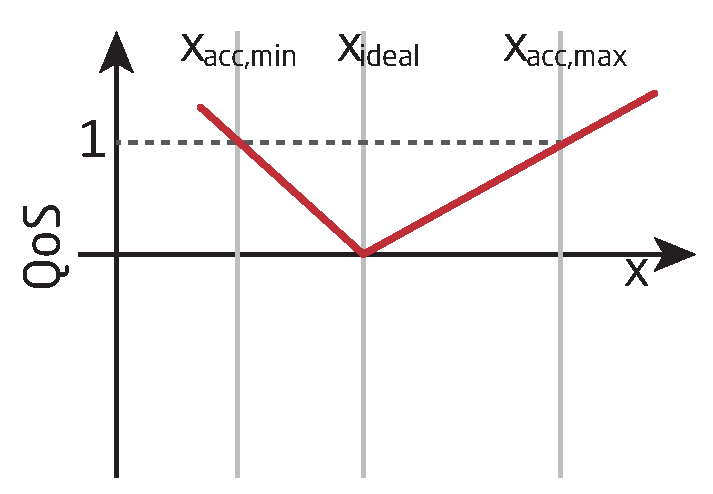
\includegraphics[width=0.5\columnwidth]{SEGAN/tracking_error3.eps}%
\label{fig:qostracking}}
\caption{Error and QoS for tracking services, note that the acceptable band do not need to be symmetric.}
\label{fig:tracking_error}
\end{figure}
\begin{figure}
\centering
\subfloat[Error]{\includegraphics[width=0.5\columnwidth]{SEGAN/band_error2.eps}%
\label{fig:errorband}}\subfloat[Quality of Service]{\includegraphics[width=0.5\columnwidth]{SEGAN/band_error3.eps}%
\label{fig:qosband}}
\caption{Error and QoS for band services.}
\label{fig:band_error}
\end{figure}
\begin{figure}
\centering
\subfloat[Error]{\includegraphics[width=0.5\columnwidth]{SEGAN/cap_error2.eps}%
\label{fig:errorcap}}
\subfloat[Quality of Service]{\includegraphics[width=0.5\columnwidth]{SEGAN/cap_error3.eps}%
\label{fig:qoscap}}
\caption{QoS for a maximum cap service, a minimum cap service is defined similarly but with $x_{min}$ and $x_{acc,min}$ values.}
\label{fig:cap_error}
\end{figure}
%\begin{figure*}[!t]
%\centerline{\subfloat[Case I]\includegraphics[width=2.5in]{subfigcase1}%
%\label{fig_first_case}}
%\hfil
%\subfloat[Case II]{\includegraphics[width=2.5in]{subfigcase2}%
%\label{fig_second_case}}}
%\caption{Simulation results}
%\label{fig_sim}
%\end{figure*}

Note that in \eqref{eq:cst}, $C_{s}(t)$ is not defined for $x_{acc}(t) = x_{ideal}(t)$. This is a corner case, in which:
%\bondynote{This QoS is only used then to calculate the Non-Delivery K, so, since we subtract 1 later on anyway, we might as well say the cornercase automatically starts counting on the Non-Delivery, and QoS = 1 for $e \neq 0$}
\begin{equation}
QoS(t) = e(t), \quad x_{acc}(t) = x_{ideal}(t)
\end{equation}


\subsection{Assessing service delivery}
Having defined an instantaneous measure for the quality of individual services, we can evaluate the aggregator as a whole based upon the quality of all the services it delivers. The chosen requirements for such and index are \cite{bondy2014performance}:
\begin{itemize}
	\item[R1] Provide a \emph{quality} measure normalized to the contractual requirements (bounds) of a service. 
	\item[R2] The measure should be normalized with respect to time.
	\item[R3] Provide a \emph{reliability} measure in relation to service non-delivery.
	\item[R4] Each service must have a separate, individually verifiable, measure. For example, to evaluate service delivery w.r.t. ancillary-service delivery, the asset-management quality is irrelevant.
\end{itemize}

The overall service delivery index of AS is defined by $\eta^{AS}$ in Eq.~\eqref{eq:etaAS}, but before calculating the index the QoS must be cleaned. To sort out non-delivery incidents (which are measured apart), we clamp $QoS_{K,meas}^{AS}(t)$ (the measured quality of service for the \emph{K} ancillary services the aggregator is providing) such that it does not account for $QoS \geq 1$: 
\begin{algorithmic}[H]
\FOR{ t = 0:$t_N$ }
\FOR{ i = 1:K}
    \IF{$QoS_{i,meas}^{AS}(t)>1$} 
        \STATE $QoS_{i}^{AS}(t) = 1$ 
    \ELSE 
        \STATE $QoS_{i}^{AS}(t) = QoS_{i,meas}^{AS}(t)$
    \ENDIF
\ENDFOR
\ENDFOR
\end{algorithmic}
where \emph{K} is the total number of AS the aggregator provide.
This clamping is not done in \cite{bondy2014performance} since that work did not use of a separate non-delivery index. This means that $\eta_{AS}$ is only a measure of the service provision performance within the contractual limits.

While the previous definitions have been established in continuous time, the actual measurement and calculations are done in discrete time. This leads to $\eta_{AS}$ being estimated for \emph{K} amount of AS over each corresponding discrete time horizon $N_K$:
\begin{align}\label{eq:etaAS}
\eta^{AS} &= \sum^{K}_{i=1} W_i \sqrt{\frac{\sum^{N_i}_{t=0} \left( {QoS^{AS}_{i,t}}^{2} \right)}{N_i}}\\
\sum_{i=1}^K W_i &= 1
\end{align}

where $W_K$ is the assigned weight to each AS, leading to $\eta^{AS} \in [0,1]$, and $\eta$ close to zero representing good performance while $\eta$ close to 1 representing a barely acceptable performance. This means that the service performance assessment index for all the AS the aggregator provides is a weighted average of the root mean square (RMS) of the error in all service deliveries. With this index it is possible to evaluate aggregators that deliver more than one AS at a time, e.g. a frequency containment reserve and a replacement reserve, and assign a hierarchy of importance with respect to the services. However, how to do distinguish measurements to verify the services, and how to evaluate which service is more important, is out of scope of this work, but the definition of Eq.~\eqref{eq:etaAS} takes the possibilities into account. In the case where only a single service delivery is considered, Eq.~\eqref{eq:etaAS} is simply the RMS of the error in service delivery:
\begin{equation}\label{eq:etaASsimp}
\eta^{AS} = \sqrt{\frac{\sum^{N}_{t=0} \left( {QoS^{AS}_{t}}^{2} \right)}{N}}.
\end{equation}

Similarly, the ability of the aggregator to deliver AMS as a whole can be measured with an index $\eta^{AMS}$ (Eq.~\eqref{eq:etaAMS}). In this instance, QoS is also clamped to $QoS^{AMS}_{M}(t) \in [0,1]$, and the amount of \emph{M} services are evaluated for their corresponding time horizon $N_M$:
\begin{equation}\label{eq:etaAMS}
\eta^{AMS} = \sum^{M}_{i=1} W_i \sqrt{\frac{\sum^{N_i}_{t=0} \left( {QoS^{AMS}_{i,t}}^{2} \right)}{N_i}}
\end{equation}
with $\eta^{AMS} \in [0,1]$. Each of these indices give an idea of the performance of the aggregator where the duration of time delivery is taken into account. This means that two service provisions are evaluated equally when their error in service delivery compared to the duration of the service delivery are the same. With these definitions, requirements \emph{R1}, \emph{R2} and \emph{R4} are fulfilled.

Finally, if the aggregator desires to have an internal overall evaluation of all the services it is providing, it can do so through a weighted mean of the service performance indices:
\begin{equation}
\eta_{tot} = \alpha \eta^{AS} + (1-\alpha) \eta^{AMS}, \quad \alpha \in [0,1]
\end{equation}
where $\alpha$ is the weight ratio the aggregator assigns to the performance of the services.

\subsection{Verifying service delivery}
Requirement \emph{R3} mentioned in the previous section asks for a reliability measure. To address this requirement, an index $\epsilon^{AS}$, similar to the service performance assessment index, is defined for verifying the delivery of AS\footnote{This can also be interpreted as evaluating non-delivery of service.} and an index $\epsilon^{AMS}$ is defined for the verification of AMS. Also, a non-delivery measure for the AS provision, $ND^{AS}$, is defined according to the following pseudo code:

\begin{algorithmic}[H]
\FOR{ t = 0:$t_N $}
\FOR{ i = 0:K}
    \IF{$QoS^{AS}_{i,meas}(t)<1$} 
        \STATE $ND^{AS}(t) = 0$ 
    \ELSE 
        \STATE $ND^{AS}(t) = QoS^{AS}_{i,meas}(t)-1$
    \ENDIF
\ENDFOR
\ENDFOR
\end{algorithmic}
This clamping shows that whenever the QoS of a service exceeds 1, i.e. the limit of what is an acceptable service provision, the amount with which it breaks the acceptable constraint is measured by \emph{ND}.
$\epsilon^{AS}$ is calculated in the same way as $\eta^{AS}$ using $ND^{AS}_K(t)$ instead of $QoS^{AS}_{K}(t)$:

\begin{equation}\label{eq:epsilonAS}
\epsilon^{AS} = \sum^{K}_{i=1} W_i \sqrt{\frac{\sum^{N_i}_{t=0} \left( {ND^{AS}_{i,t}}^{2} \right)}{N_i}}
\end{equation}
where $\epsilon^{AS} \in [0,\infty]$.

The same clamping process is applied to the non-delivery measure of the AMS, and $\epsilon^{AMS}$ is defined as:
\begin{equation}\label{eq:epsilonAMS}
\epsilon^{AMS} = \sum^{M}_{i=1} W_i \sqrt{\frac{\sum^{N_i}_{t=0} \left( {ND^{AMS}_{i,t}}^{2} \right)}{N_i}}.
\end{equation}

Thus $\epsilon$ is used to asses the severity of non-delivery events. For some systems it is critically important that $QoS(t)\leq1$ at any time, in which case $\epsilon$ should be close to zero for the contract to be considered respected. Other systems can tolerate $QoS(t)>1$ for some period, which leads to a higher acceptable $\epsilon$. A service delivery is verified if $\epsilon \leq \epsilon_{max}$, and this contractual limit, i.e. the value of $\epsilon_{max}$, must be assessed individually depending on the nature of the system. It is likely that in most cases $\epsilon^{AS}_{max}<\epsilon^{AMS}_{max}$, since the security of the power system is more important than, e.g., the temperature comfort of a home owner.

In \cite{bondy2014performance}, non-delivery is assessed using a non-delivery counter (NDC). $\epsilon$ differs from the NDC in that it both captures the time span of non-delivery and the magnitude of the violation, whereas NDC only captures the amount of time samples where non-delivery is detected. $\epsilon$ might prove advantageous over the NDC as a service verification index for some systems. A disadvantage of $\epsilon$ is that it might be a less intuitive measure to communicate to the service providers compared to the NDC.

Fig. \ref{fig:RefErr} shows an example of reference tracking error service performance assessment. Deviations between $x_{act}$ and $x_{ideal}$ inside the band defined by $x_{acc}$ will lead to $QoS<1$, while deviations outside the $x_{acc}$ band will lead to $QoS>1$. For this particular example $\eta^{AS}=0.7501$ and the service verification index is $\epsilon^{AS}=0.2324$, which indicates that generally the service provision is bad at following the reference, and also has a moderate amount of non-delivery. The service acquirer will have to decide whether this verification index value is acceptable or if it should lead to economical penalization or contract termination.

\begin{figure}
\centering
\includegraphics[width=\columnwidth]{SEGAN/reftrack.eps}
\caption{Example of reference tracking error with performance $x_{act}$, ideal performance $x_{ideal}$ and tolerance limits $x_{acc}$.}
\label{fig:RefErr}
\end{figure}


\section{Case Studies}\label{sec:SEGANcasestudies}
Using two different ancillary services and an asset management service as cases, we will illustrate the utility of the generic service modeling method, the service performance index and the service verification index. The first case study focuses on frequency containment reserve in western Denmark, the second focuses on the theoretical PowerMax DSO service, and the third focuses on the temperature management of a residential house. 

\subsection{Frequency Containment Reserve in Western Denmark}
Frequency Containment Reserve (FCR) is utilized to contain frequency excursions deviating from the nominal 50 Hz in \emph{ENTSO-E RG Continental Europe’s synchronous area} of which western Denmark (DK1) is part of. The Danish TSO, Energinet.dk, is obliged to provide a proportional share of $\pm$ 23 MW \cite{EnerginetAncillary} out of the total synchronous area need of $\pm$ 3000 MW. Energinet.dk buys these reserves at daily auctions. The service specifications are defined in \cite{EnerginetAncillary}.

The six steps outlined in Sec.~\ref{sec:SEGANmethodology} are used to model the ideal and tolerated service response. 1) The physical parameters are grid frequency (accuracy of $\pm$ 10 mHz or better), generator reserve power output, and timing of service delivery (accuracy of 1 s or better). 2) The reserve must be supplied linearly at deviations of $\pm$ 200 mHz relative to 50 Hz, with a $\pm$ 20 mHz dead-band around 50 Hz. 3) The physical size of the service depends on the reserve bid size. This work will look at a generic reserve bid. According to the discussion from Eq.~\eqref{eq:QoS}, $x_{ideal}$ cannot be equal to $\mathbf{x}_{acc}$. Therefore, a $\pm$ 1\% tolerance band of $x_{ideal}$ is assumed. 4) The first 50\% of the service must be supplied within 15 s and 100\% must be supplied within 30 s. The ideal response can be defined as a response with an instant 100\% power ramp \cite{makarov2008assessing}. 5) The ideal and tolerated response of this service provision is plotted as $x_{ideal}$, $x_{acc,min}$ and $x_{acc,max}$ in Fig.~\ref{fig:DK1PrimResSim}, which assumes that a reserve power set-point has already been established based on the values from step 2.%Fig.~\ref{fig:DK1PrimResDyn}

%\begin{figure}
%\centering
%\includegraphics[width=\columnwidth]{figures/dynresp.eps}
%\caption{DK1 Primary Reserve service provision curve. The curve shows the relationship between the activated fraction of the primary reserve bid, and the grid frequency, including the +/- 20 mHz dead-band. This should not be confused with the droop curve.}
%\label{fig:DK1PrimResDyn}
%\end{figure}

Fig. \ref{fig:DK1PrimResSim} shows a simulation of primary regulation active power ramp $x_{act}$ for the time interval $[-5,35]$ s. The service delivery performance index and non-delivery verification index are $\eta^{AS}=0.4257$ and $\epsilon^{AS}=0.1392$, calculated using Eq. \eqref{eq:etaAS} and Eq.~\eqref{eq:epsilonAS}. The TSO must determine a threshold $\epsilon_{max}$, such that the service provider is penalized or the contract is terminated if $\epsilon^{AS}>\epsilon^{AS}_{max}$. It is not the scope of this work to asses a suitable value of $\epsilon^{AS}_{max}$.%\bondynote{We are repeating ourselves a bit here}

\begin{figure}
\centering
\includegraphics[width = \columnwidth]{SEGAN/primfreqresp.eps}
\caption{Simulation of a DK1 primary reserve power ramp response together with $x_{ideal}$ and $x_{acc}$ values.}
\label{fig:DK1PrimResSim}
\end{figure}

\subsection{PowerMax in a distribution system}
The \textit{PowerMax} service was first described in \cite{ding2013development} and further specified in \cite{bondy2014flech}. It is a DSO service, where the DSO can make a tender for a load reduction $\Delta P^{DSO}$ to a max level $P_{max}^{DSO}$ in parts of the distribution system that are forecasted to experience congestions during some periods (e.g. hours 17-20 during winter months). The motivation for \textit{PowerMax} is that the service could be an economically beneficial alternative to grid reinforcements in some situations. This is both due to saved interest and depreciation on investments plus the avoided risk of over-sizing equipment in case of future energy savings or if the disappearance of a large consumer makes the reinforcement unnecessary.% The tender is announced and cleared through Flexibility Clearing House (FLECH), where flexibility aggregators can bid on the tender.%where the service is delivered by aggregator companies, which bid in flexibility from a group of units which they control. 

%Following is a mathematical definition of the \textit{PowerMax} service, as previously developed in \cite{bondy2014powermax}. 
In order to identify its service needs, it is assumed that the DSO is able to separate the total consumption forecast $\hat{P}_{tot}$ in the congested part of the distribution grid into a controllable load forecast $\hat{P}_{CL}$ and a base load forecast $\hat{P}_{BL}$:
\begin{align}
\hat{P}_{tot} &= \hat{P}_{CL} + \hat{P}_{BL} \\
\hat{P}_{CL} &= \sum_{Agg} \hat{P}_{CL,Agg}, \quad Agg \in \mathbf{A} \label{eq:CLDef}
\end{align}
where $\mathbf{A}$ is the set of all aggregators in the considered part of the grid. Only the aggregators \emph{Agg} that bid for the service tender make up $\hat{P}_{CL}$, while the rest of $\mathbf{A}$ is part of $\hat{P}_{BL}$. The aggregators must be contracted to deliver a total power reduction $\Delta P$, such that the system operational limit $\bar{P}_{sys}$ is not violated by the peak base load forecast and the peak controllable load forecast:

\begin{equation}
\hat{\bar{P}}_{BL}+\hat{\bar{P}}_{CL}-\Delta P \leq \bar{P}_{sys}. \label{eq:PSysDef}
\end{equation}

This inequality can be fulfilled by setting a peak limit $\bar{P}_{CL}$:
\begin{equation}
\bar{P}_{CL} = \hat{\bar{P}}_{CL} - \Delta P \label{eq:PBarCLDef}
\end{equation}
where $\Delta P$ and $\bar{P}_{CL}$ are the variables for the DSO service tender. In order to formulate a service tender, the magnitude of these variables must be estimated taking into account the uncertainty of the forecasts, giving the following expressions:
\begin{align}
\Delta P^{DSO} &= \sum_{Agg} \Delta \hat{P}_{CL,Agg} + \text{Risk\{}\hat{P}_{CL} + \hat{P}_{BL}\text{\}}\\
P_{max}^{DSO} &= \hat{\bar{P}}_{CL} - \Delta P_{DSO}
\end{align}
where $\Delta \hat{P}_{CL,Agg}$ is the estimated power reduction for the individual aggregator bid, $\text{Risk\{}\hat{P}_{CL} + \hat{P}_{BL}\text{\}}$ is the risk associated to the load forecast uncertainty. $Agg \in \mathbf{A_{C}}$ and $\mathbf{A_{C}} \subseteq \mathbf{A}$, i.e. $\mathbf{A_{C}}$ is the subset of aggregators that bid on the tender. After the DSO has identified a suitable $P_{max}^{DSO}$ and $\Delta P^{DSO}$ to solve the congestion issue, the DSO formulates a service tender for which aggregators can bid their corresponding $\Delta P^{Agg}$ and $P^{Agg}_{max}$. %The DSO sets a maximum price it is willing to pay for the load reduction, which is related to the alternative cost of grid reinforcements. In case the market is not cleared at or below the maximum price, the DSO can formulate a new tender, adjusting the risk value, POD (point of delivery) list or amount of power reduction. The timing of the tender process should be such that the DSO has time to conduct grid reinforcements as an alternative.

The method from Sec.~\ref{sec:SEGANmethodology} is used to model \textit{PowerMax} ideal and acceptable response. 1) The physical parameters are $P_{max}^{Agg}$, $\Delta P^{Agg}$ and months/days/hours the service shall be delivered. 2) The system does not posses a dynamic behaviour related to system parameters. 3) As an example, the service tender defines $P_{max}^{Agg} = 200$ kW and $+1\%$ allowed deviation $P_{max,acc}^{Agg}$. 4) In this example we use 120 min service provision time with allowed non-delivery in the first 15 min, and the last 5 min, of the service delivery (following the service definition in \cite{ding2013development}) and the ideal service delivery is the one that respects $P_{max}^{DSO}$. 5) Figure \ref{fig:PowerMaxSim} plots $x_{ideal}$ and $x_{acc}$. The \textit{Activation Dead-band} indicates the regions where the aggregator is not obliged to deliver the service because of the tolerances defined under step 4. 6) The service is a maximum cap service and the error is measured as in Eq.~\eqref{eq:maxmin_cap}.

An example of a load curve $P_{Agg}=x_{act}$ is presented in Fig.~\ref{fig:PowerMaxSim}. The service delivery and verification are evaluated using Eq.~\eqref{eq:etaAS} and Eq.~\eqref{eq:epsilonAS}, yielding $\eta^{AS} = 0.5074$ and $\epsilon^{AS} = 0.2701$ respectively. As with the performance assessment of the FCR in DK1, it is not within the scope of this paper to asses the value of $\epsilon^{AS}_{max}$, yet a qualified assessment can be made. %, which will lead to either penalization or termination of the contract.
To asses $\epsilon^{AS}_{max}$, the DSO must analyze the dynamics of the problem the service is helping relieve. For \textit{PowerMax}, the dynamics are governed by the heating of the overloaded equipment (e.g. transformer or cable), which deteriorates over time due to overheating. A feeder might be tolerant to short term overloads and therefore the DSO might set $\epsilon^{AS}_{max}$ higher than in the FCR case.

\begin{figure}
\centering
\includegraphics[width = 0.86\columnwidth]{SEGAN/powermaxsample.eps}
\vspace{-4pt}
\caption{$x_{ideal}=P_{max}^{Agg}$, $x_{acc}=P_{max,acc}^{Agg}$ for the considered \textit{PowerMax} example. The activation Dead-band is the time period, where the aggregator is allowed to non-deliver.}\label{fig:PowerMaxSim}
\end{figure}

\subsection{Temperature management of a flexible household}
Household heating is a flexible process where the thermal capacity of the building can be considered a form of energy storage. In Denmark, heat pumps are being installed with the capability of being remotely controlled by an aggregator, see e.g. \cite{insero}. It is assumed that the aggregator will help the heat pump owners to maintain a comfortable indoor temperature and utilize the electric consumption flexibility in exchange of monetary compensation.

Applying the method from Sec.~\ref{sec:SEGANmethodology} to model the service: 1) The physical parameters are the minimum and maximum of the temperature comfort bands of the household. 2) The service does not posses a dynamic behaviour related to system parameters. 3) As an example, the household owner sets a comfort band of $\mathbf{x}_{ideal} = [x_{min},x_{max}] = [20 ^{\circ}\text{C},22^{\circ}\text{C}]$ and allows for a $\pm 1 ^{\circ}\text{C}$ as acceptable error. Furthermore, the owner decides that during the night, the house can be two degrees colder. 4) In this example the ideal response is performance within the temperature bounds. 5) Fig.~\ref{fig:tempband} plots $x_{ideal}$ and $\mathbf{x}_{acc}$. 6) The service is a band service and the error is measured according to Eq.~\eqref{eq:band_error}.

The service model and the actual temperature of a simulation can be seen in Fig.~\ref{fig:tempband}, where it is clear that generally the aggregator is able to provide a reasonable service performance, with no non-delivery ( $\eta^{AMS} = 0.2707$ and $\epsilon^{AMS} = 0.0$). As described in Sec.~\ref{sec:DERs}, the aggregator may be in charge of the overall control of a cluster of units, in which case the performance should be evaluated over the whole cluster. To show this, simulations are done for 20 households and the equally-weighted average of the indices results in $\eta^{AMS} = 0.2411$ and $\epsilon^{AMS} = 0.0211$ (Fig.~\ref{fig:tempbandclustererror}).

\begin{figure}
\centering
\includegraphics[width = \columnwidth]{SEGAN/tempband.eps}
\caption{Simulation of the indoor temperature of a Danish household.}
\label{fig:tempband}
\end{figure}

\begin{figure}
\centering
\includegraphics[width = \columnwidth]{SEGAN/tempbandclustererror.eps}
\caption{Simulation of the indoor temperature of 20 Danish households. The mean temperature is plotted, along with the minimum and maximum values of the cluster.}
\label{fig:tempbandclustererror}
\end{figure}


\section{Conclusion}\label{sec:SEGANconclusion}
This paper presents a generic method for modeling ancillary services for evaluating the performance of a service provision. The performance is assessed by means of a service performance assessment index and a service verification index. The use of the modeling method and the indexes are illustrated with three case studies covering a traditional ancillary service, a new distribution system service and an asset management service. The main purpose behind the development of the modeling method and the indices is to provide key components in a framework for prequalification of aggregator algorithms. As the framework is developed, the usefulness of the presented concepts will be shown and reiterated upon in case shortcomings are found. The performance assessment of aggregators in terms of the services they are to provide is therefore an important element in integrating new sources of ancillary services in the power system. These new sources are expected to play an important part in the security of the future power system. %The usefulness of the indexes might be further investigated and the method revised by means of laboratory tests and small scale demonstrations on units connected to the power grid.



\section*{Acknowledgment}
Parts of this work are supported by the Programme for Energy Technology Development and Demonstration (EUDP) through PowerLabDK and Innovation Fund Denmark through the iPower project. The authors thank Antonio Zecchino and Henrik W. Bindner for reviewing the draft of the paper.



%!TEX root = ../Thesis.tex
\chapter{Performance Assessment of Aggregation Control Services for Demand Response}\label{app:isgt2014}

\textbf{Authors:}\\
Daniel Esteban Morales Bondy\\
Giuseppe Tommaso Costanzo\\
Kai Heussen\\
Henrik W. Bindner

\noindent
\textbf{Published at:}\\
Innovative Smart Grid Technologies Conference Europe (ISGT-Europe), 2014 IEEE PES\\
Istanbul, Turkey

\noindent
\textbf{Abstract:}\\
Aggregation algorithms that provide services to the grid via demand side management are moving from research ideas to the market. With the diversity of the technology delivering such services, it becomes essential to establish transparent performance standards from a service delivery perspective. This paper formulates performance measures and an index to evaluate in hindsight the quality of service delivery by an aggregator, both with respect to ancillary service and asset management service.


The index is based on requirements formulated in service contracts and provides an overall assessment of the quality of service provided by an aggregation control algorithm. By a detailed case study we present and an application of the index, comparing the performance of two different control architectures for demand side management delivering a distribution grid service.
\section{Introduction}

%Denmark has set as an objective that by 2050 the country should be independent of fossil fuels[source!, reformulate]. The integration of Renewable Energy Sources (RES), such as wind turbines and photovoltaic cells, and Distributed Energy Resources (DERs), such as EVs and heat pumps, will be integral to achieve this goal.

	The future increase in energy production from Renewable Energy Sources (RES) may lead to a power system where production is distributed, and where the Transmission System Operators (TSOs) require a larger amount of balancing services. At the same time, the increase in Distributed Energy Resources (DERs) brings new challenges to the Distribution System Operators (DSOs), which may need new kinds of ancillary services\cite{ipower2013development}. It is anticipated that DER owners will be able to provide services to the system operators via Demand Side Management (DSM). 

An Aggregator is a market player, or market role, whose business case is to manage DER units in its portfolio and use their inherent consumption flexibility to participate in the ancillary service markets, i.e. it controls units in order to perform DSM. A general classification of different aggregation methods is presented in \cite{kosek2013overview}, an example of direct control can be found in \cite{Biegel}, and an analysis and evaluation of indirect control architectures can be found in \cite{Heussen}.

Since the Aggregator has contractual obligations with customers and system operators, it is important that the control algorithm the Aggregator uses proves suitable for the task. From a service perspective, an aggregation algorithm is considered suitable if the performance, i.e. the quality of service (QoS), it delivers is within the contractual limits. The Aggregator must therefore control its DER portfolio in such a way that it fulfills the needs of both the DER owners and the System Operator.% The bounds of the QoS delimit the acceptable service provision, which is essential to the functioning of the power grid.

Little attention has been given to the problem of performance assessment of aggregator controllers seen from a service-delivery perspective. This paper approaches the problem by presenting two main ideas:
\begin{itemize}
	\item both ancillary services and DSM have minimum QoS requirements that need to be respected. In this work we propose a way of modeling the service requirements so that the quality of service delivery can be measured;
	\item a performance index suitable for evaluating the quality of aggregation control algorithms from point of view of the Aggregator.
\end{itemize}

The paper is organized as follows: Section \ref{sec:method} gives a general description of concepts relevant to the definition of the index, while the index itself is defined in Section \ref{sec:index}. A case study is presented in Section \ref{sec:case} and further research is discussed in Section \ref{sec:conclusion}.


\section{Background} \label{sec:method}

	\subsection{Ancillary Services} % (fold)
	\label{sub:ancillary}
	Ancillary services are acquired by TSOs in order to ensure the stability of the system and they can generally be divided into primary, secondary and tertiary ancillary services \cite{Rebours}. Each class of ancillary services has a different purpose in grid operation and works on different time scales.

	In the Danish system, producers, represented by a Balance Responsible Party (BRP), are allowed to bid into the ancillary-services market once they have been approved by the TSO. In order to be approved, the producers must prove that they are able to deliver the relevant services within the requirements defined in \cite{EnerginetAncillary,bondy2013}. Here, the TSO defines the bounds of error in service delivery, e.g. how much deviation with respect to a reference power schedule can be accepted before the service is considered non-delivered. In this work, the QoS measures the deviations from the contracted behavior.

	Furthermore, it is expected that new ancillary services will appear in the near future \cite{FLECH}. The two main problems that the DSO seeks to solve are congestion issues, i.e. overloading of cables or transformers, and voltage issues. Throughout this paper, the recurring example of an ancillary service is the \emph{PowerMax}, one of the new DSO services. This service is discussed further in Sec.\ref{sub:example}.
	% subsection ancillary_services (end)
	
	\subsection{Asset Management Service} % (fold)
	\label{sub:asset}
	Since the flexibility of individual DERs is too small to provide services to the system operators, an Aggregator pools the flexibility of the units, and presents their flexibility in the market as a single entity, see Fig.\ref{fig:systemarch}. Thus, the Aggregator is responsible for managing the DER units according to certain requirements defined by the owners, hereby providing an asset management service. This service must respect the primary function of the DER. 
	
	By changing the consumption behavior of DER units, the Aggregator performs Demand Side Management (DSM), providing ancillary services to the DSO or, through a BRP, the TSO. The Aggregator and the BRP could be the same entity, but if they are not, the Aggregator should not work against the balancing responsibilities of the BRP.  
	
	\begin{figure}[t]  % Find out how to send it to next column.
		\centering
		\includegraphics[width=0.7\textwidth]{isgt2014/system.eps}
		\caption{The setup of the power system with DSM. Note that the Aggregator can either be an independent entity or can be a role inside a BRP.}\label{fig:systemarch}
	\end{figure}
	
%	The objective of a DER is to satisfy the needs of its owner. The Aggregator provides the DER owners with an asset management service that ensures the QoS to customers is adequate. Providing services to the grid is only a secondary (and optional) function of the DER, which the Aggregator must take advantage of within the constraints of the primary function. 
	
%	The power consumption of DERs varies greatly depending on the daily routines of their owners and the meteorological conditions. Due to the varying load size, behavior and distributed nature of the DERs, the Aggregator must be able to evaluate if its control algorithms are capable of providing ancillary services and asset management satisfactorily.

	% subsection asset_management_service (end)
	
	\subsection{Control Performance Assessment}
	There is a field of theory on evaluation of controllers: Control Performance Assessment (CPA). Applications of this theory are found mostly in the process industry; for a thorough overview of its applications we refer to \cite{Jelali,Green}. 

		Typically, CPA methods fall within two approaches. One approach, first introduced in \cite{Harris1989}, is to benchmark controller performance against a theoretical optimum, while taking the stochasticity of the system into account. The second approach is to benchmark against deterministic properties the closed-loop system must have, e.g. settling time and steady-state error \cite{Astrom}. In both cases, the index is usually scaled such that:
\begin{equation}
	\zeta = \frac{J_{opt}}{J_{act}},\label{eq:astrom}
\end{equation}
where $J_{opt}$ is the theoretical optimal (minimum) value of the performance criterion \emph{J} (which is usually impossible to achieve in reality), and $J_{act}$ is the actual measured value of the criterion. Since $J_{opt}<J_{act}$, then $\zeta \in [0,1]$. 
		%Given that the requirements of service delivery are easily translated into time-domain deterministic measures, this work presents a deterministic approach. Using the concepts presented in this section, the performance index is defined in the next section.
%In the following, we propose the application of CPA concepts to DSM.

		According to \cite{Green}, performance criteria used to evaluate a controller usually fall within three categories: Quality, Reliability, and Energy. Quality and reliability are concepts that can be directly related to ancillary service provision. The interpretation of energy-related criteria may be suitable for asset-management purposes but is considered out of scope in this work.% The quality of the control performance is measured by the QoS it provides, both towards the system operators and towards its customers. Reliability is measured as how many times the controller provides a QoS outside the specified limits.

\section{DSM Performance Assessment} % (fold)
\label{sec:index}
We identify four requirements for performance assessment of DSM:
\begin{itemize}
	\item[R1] Provide a \emph{quality} measure normalized to the contractual requirements (bounds) of a service. By normalizing the quality measure to the bounds, the \emph{QoS} value for both ancillary services and asset-management services will have comparable dimensions.
	\item[R2] The measure should be normalized with respect to time.
	\item[R3] Provide a \emph{reliability} measure in relation to service non-delivery.
	\item[R4] Each service must have a separate, individually verifiable, measure. For example, to evaluate service delivery w.r.t. ancillary-service delivery, the asset-management quality is irrelevant.
\end{itemize}

To satisfy these requirements, we propose a performance index quantifying the quality of ancillary services and asset-management services, and a non-delivery counter (NDC) which increases every time the QoS is out of bounds. Normalization is based on a scaling factor modeled after the contractual limits of the respective service. The limits are defined via a contract with the entity requesting the service. Thus, the performance index is specifically designed to evaluate how well the service provision conforms to the contractual boundaries.
	%The formulation of a performance index transforms the service requirements of the Aggregator into a single computable quality measure. %The index presented here is defined for post-simulation analysis, and represents the performance of the control algorithm over the whole time horizon. 
	\subsection{Definition of the performance index}
	In previous sections we have defined the concept of QoS as a deviation, $e(t)$, from a contracted behavior. Since there is a contractual limit on the allowed deviation, the error is normed to be a percentage of this limit such that:
	\begin{equation}
		QoS_{s}(t)=|e(t)|C_{s}(t); \quad  QoS_{s}(t)\in [0,1]
	\end{equation}
	where \emph{s} is either \emph{AS} for ancillary service or \emph{AMS} for asset-management service, and $C_s(t)$ is the corresponding normalization factor derived from the service model. When $QoS_{AS}(t) \geq 1$, the measure for reliability NDC is increased. %For the ancillary services this is simply expressed as $QoS_{AS}(t) = e(t)_{AS}$ while the expression for the asset management service is $QoS_{AM}(t) =\sum_{k=1}^M e(t)_{AM}$.

	Using the square root of the Integral Square Error index (i.e. the 2-norm, as defined in e.g. \cite{Skogestad}), the following performance criterion is defined for service delivery seen from the Aggregator perspective:
	\begin{equation}
		%\text{J}=\sqrt{\int_{0}^{N}\left( \sum_{k=1}^M |e(t)_{AM,k}C_{AM}|^{2}+|e(t)_{AS}C_{AS}|^{2}\right)dt} 
		{J}(N)=\sqrt{\int_{0}^{N}\left( \sum_{k=1}^M {QoS}_{AMS,k}(t)^{2}+{QoS}_{AS}(t)^{2}\right)dt} 
	\end{equation}
where ${QoS}_{AM,k}(t)$ and ${QoS}_{AS}(t)$ are the time-dependent measures of service quality for the asset-management service and the ancillary service, respectively. The units controlled by the Aggregator are denoted by the index \emph{k}, the unit portfolio is of size \emph{M}, and \emph{N} is the time horizon over which the services are provided. %Finally, $Q_D$ and $Q_U$ are scaling factors that convert the errors into percentages so that $e(t)_D$ and $e(t)_U$ are comparable. 
While the index~\eqref{eq:astrom} benchmarks the actual performance criterion against a theoretical minimum, we benchmark it against the worst case scenario $J_{max}$, such that the performance index is given by:
	\begin{equation} 
		\eta = \frac{J_{act}(N)}{J_{max}(N)}\label{eq:eta}
	\end{equation}
	where $\eta \in [0,1)$ for a valid service delivery and for which values close to zero represent good performance of service delivery. If $\eta \geq 1$ the Aggregator does not perform according to its service contract.
		
		Normalization with respect to time is achieved when benchmarking against $J_{max}(N)$, since $J_{max}(N)$ is estimated by integrating over the service delivery period. Contrary to index \eqref{eq:astrom}, which gives an intuition of how close performance is to the optimum, index \eqref{eq:eta} gives an intuition of how far performance is from the worst case scenario. The index is designed this way because the theoretical optimum of service delivery is $J_{opt}=0$, i.e. no error in service delivery.
	%It must be noted that the performance criterion only measures the permissible error defined in the contract of the service (the service quality), and service non-delivery (the service reliability) is measured separately. Therefore, whenever the algorithm performs outside the established limits, then $J(t)_{act}=J(t)_{max}$ and a non-delivery counter is increased.
	\subsection{Calculating the index}\label{sub:modelcalc}
	Having defined what the performance index measures, we will proceed with establishing how to obtain the required values to estimate the index. Calculating the performance index requires the following steps:
	% the maximum permissible error ($J(t)_{max}$) of the service requires two steps:
		\begin{enumerate}
		\item Identify and model the service requirements and errors in service provision, giving the scaling factor $C(t)_s$.
			\item Estimate $J_{act}(N)$.
			\item Calculate \emph{J(N)} for operation on the requirement boundaries ($J_{max}(N)$).
			\item Calculate $\eta$ by benchmarking $J_{act}(N)$ with $J_{max}(N)$.
		\end{enumerate}	
		
	For the first step, the service requirements must be defined and translated into measurable errors. For some services, the error can be stated as a tracking error, e.g. $e=y_{ref}-y_{meas}$. In other cases, service requirements are defined by operation within bands, which may lead to an error defined as:
	\begin{equation}
	e(x)= \left\{ \begin{array}{l l}
	x_{min} - x & \quad \text{ if } x \leq x_{min}\\
	0 & \quad \text{ if } x_{min} \leq x \leq x_{max}\\
	x - x_{max} & \quad \text{ if } x \geq x_{max}
	\end{array} \right.
	\end{equation}
	This step is a service-specific problem and is non trivial.

	The second step requires computing $J_{act}(N)$ using measurement data from the unit portfolio. This can be a challenge for evaluation in field deployment. In this paper it is assumed that the measurement data is available, either through a DSO or a third-party metering company.	
	
		%The actual performance of the aggregation algorithm can be found through two different methods:
%\begin{itemize}
	%\item On-line monitoring -- This method brings the added benefit of being able to use the index for performance monitoring and diagnosis at runtime, but the downside of being communication intensive.  
	%\item Post-delivery analysis -- This method is less communication intensive, but does not permit to take remedial actions at run time if a aggregation controller is not working as expected.
%\end{itemize}
%	Usually services have some acceptable error (see Sec.~\ref{sub:ancillary}) which can be interpreted as the hard boundaries for the service delivery.
	The third step requires the calculation of \emph{J(N)} along the contractual boundaries for service delivery, in this way, the maximum allowed error is found for the service. The boundaries are based on the service models presented in the first step. By adding the maximum permissible error for all services, $J_{max}(N)$ is obtained. 
	%Normalizing the performance measure with the $J_{max}$ gives an intuitive value of the performance of the control algorithm.
	The following subsection present an example of how to determine $J_{max}(N)$.

	\subsection{An example: DSO Service PowerMax}\label{sub:example}
	For demonstration purposes, in this section $J_{max}(N)$ for the PowerMax service is calculated. 
	Typically, the service will be contracted several months ahead of the actual delivery. The activation schedule (On and Off triggers), the maximum power cap ($P_M$), the maximum duration of the service per activation ($T_M$), and the quality of service (\emph{QoS}) are defined when contracting the service. The contract is valid for a period of several months, where the Aggregator is obliged to follow the established schedule.

	The limits specified for the QoS\cite{FLECH} of the PowerMax service are presented here: 
	\begin{itemize}
		\item Deviation from On trigger: $\pm$ 15 min. per day
		\item Deviation in size of service (dependent on $P_M$): Max. $\pm 5\% P_M$  
		\item Acceptable no. of unsatisfactory activations(non-delivery): $\text{NDC} = 4$
	\end{itemize}

A graphical representation of these service requirements is depicted in Fig.~\ref{fig:servicereq}. It is clear that the maximum acceptable error in service delivery is the shaded area. Note that the limit for non-delivery of service during the first 15 minutes of activation is dotted due to the fact that non-delivery is not counted during this period. The specifications for counting unsatisfactory activations are not clarified in \cite{FLECH}, so it is assumed that breaking the QoS limits on one sampling period counts as one non-delivery. In the case where the service is not respected in three consecutive (or non-consecutive) sampling periods, $\text{NDC}=3$.

For example, in the case where  $P_M = 5\,kW$, $T_M=4\, h$ and the power is measured once an hour, $J_{max}(N) = 2$, as it represents the square root of the square of the maximum (when $J_{act}(N)=1$) permissible error over 4 hours.
\begin{figure}[t]  % Find out how to send it to next column.
	\centering
	\includegraphics[width=2.5in]{isgt2014/drawing3.eps}
	\caption{The PowerMax service requirements, where the red line represents the boundaries for the permissible error, and the shaded area represents the error in service delivery, which is within the limits established in the QoS. }\label{fig:servicereq}
\end{figure}

	
% section the_performance_index (end)

\section{Case Study}
\label{sec:case}
This case study presents the aggregation of multiple flexible DERs via coordinated operation: 75 DERs installed in a suburban residential area, which are all connected to the same feeder leading to a 10/0.4 kV transformer. The transformer is rated to a maximum power flow of 200 kVA, which is sufficient under the current load circumstances, but will be a constraint in the future.

This case study addresses a scenario with high electric-vehicle (EV) penetration, low photo-voltaic (PV) penetration and electric space heating in all households. Furthermore all DERs connected to the same LV feeder offer their flexibility to the same Aggregator. Then, the proposed performance index for service provision is evaluated for two different aggregation control algorithms: Centralized soft Model Predictive Control (C-MPC) and Distributed soft Model Predictive Control (D-MPC).

\subsection{The reference case: without units coordination}
In this section we make a scenario hypothesis for year 2050 regarding PV and EV penetration in a distribution feeder in a rural area and present simulation results. The following units are connected to the LV transformer:
\begin{itemize}
\item 40 buildings with electric climate control: resistive space heating with maximum load of 10 kW and air conditioning with a maximum load of 5 kW.
\item 20 large EVs, with a battery size of 25 kWh, 11 kW.
\item 10 small EVs, with a battery size of 14 kWh, 3.3 kW.
\item 5 PV (polycrystalline) installations of 6 kW rated power each.
%\item 5 Li-On support batteries for local energy storage: 10 kWh, 2 kW each (95\% round trip efficiency). 
\end{itemize} 

The PV installations provide forecasts of the production for one day ahead. To simulate uncertainty in the forecasts, Gaussian noise has been added to real data of PV production according to:
\begin{equation}
	{P_{PV-F,t}} = {P_{PV-T,t}} + {v_t},\quad {v_t} \sim N\left( {0,\alpha  \sqrt {{P_{PV-T,t}}} } \right)\label{eq:pvprod}
\end{equation}
where $P_{PV-F,t}$ is the forecasted PV power production at time $t$, and $P_{PV-T,t}$ is the actual power production at time $t$ (from historical data). The term $\alpha$ is an uncertainty factor, which defines the variance of the noise as a percentage of the actual PV production, e.g. $\alpha = 0.1$ corresponds to a $10\%$ forecast error. Uncertainty in solar radiation and ambient temperature are modeled in the same way. The actual power production time-series used in this case covers the same days as \cite{costanzo2013coordination}.

The load related to households is divided into climate control (flexible load) and everything else (non-flexible load). The building climate control is operated on MPC basis for minimum deviation from the temperature set point. Regarding the non flexible household loads, a five-day (one-hour-sampled) profile of the non-flexible load of 40 households is depicted in Fig.~\ref{fig:nonflexible}.

\begin{figure}[t]  
	\centering
	\includegraphics[width=\textwidth]{isgt2014/nonflexload.eps}
	\caption{The non-flexible load of the households under the transformer. The sample is statistically representative of Danish households.}\label{fig:nonflexible}
\end{figure}

The EVs leave the charging station at a uniform randomly distributed time between 6:00  and 8:00, and are plugged again at a uniform, randomly distributed time between 16:00 and 18:00. The EVs operate on dumb charging, i.e. they try to fully charge as soon as they are connected to the grid.  %The energy price is the same for all the units within the same cluster.
By running a simulation of the described scenario without units coordination, the results shown in Fig.~\ref{fig:referencecase} are obtained.

\begin{figure}[t]  
	\centering
	\includegraphics[width=\textwidth]{isgt2014/referencecase.eps}
	\caption{Aggregated power flow at the point of common coupling for the reference case units without coordination: Demand Response based on day-ahead energy price.}\label{fig:referencecase}
\end{figure}

EVs operating on dumb charging can cause peak consumption up to 190 kW at the point of common coupling (PCC). Given that the transformer capacity is 200 kW and it is customary to reserve 30\% of the transformer capacity for emergency operations \cite{Engel}, the DSO aims at keeping the load below 140 kW and limiting the inverse power flow at the substation. Thus, the DSO can sign a contract for PowerMax service (see Sec.~\ref{sub:example}) with an Aggregator which, at any time, operates Demand Response via Direct Load Control (DLC)~\cite{kosek2013overview} in order to limit the power flow at the transformer. The maximum capacity available at the transformer is therefore 140 kW for direct power flow and -10 kW for inverse power flow.

The rest of this section presents the C-MPC and D-MPC formulations. For the formulation of the mathematical models we refer to~\cite{6345063} for the battery model and to~\cite{Bacher20111511} for the building space heating model (modified, as proposed in~\cite{costanzo2013coordination}). For the modeling of the services, we apply the method described in Sec.\ref{sub:modelcalc}. A discussion on the simulation results concludes this section.
\subsection{The Centralized Model Predictive Control scheme}
\begin{figure}[t]  
	\centering
	\subfloat[The setup of the Centralized MPC scheme.]{\includegraphics[width=1.0\textwidth]{isgt2014/centralized.eps}\label{fig:centralized}}
\\
\subfloat[The setup of the DMPC scheme as seen in \cite{costanzo2013coordination}.]{\includegraphics[width=1.0\textwidth]{isgt2014/blackboard.eps}%
\label{fig:blackboard}}
\caption{The setup of the two Aggregation algorithms to be compared.}\label{fig:systemsetup}
\end{figure}
In this scheme the Aggregator contains the control algorithm to centrally manage all the units in its portfolio (Fig.~\ref{fig:systemsetup}(a)). Since the Aggregator optimizes its portfolio's consumption through MPC, it has detailed knowledge of the state and dynamics underneath.
The units portfolio is the same as of the reference case. The C-MPC control problem is formulated as quadratic optimization with soft constraints (as seen in e.g. \cite{prasath2009a}):
{%\footnotesize
{\begin{subequations}\label{Eq: building_MPC}
\begin{align}
& \min\limits_{u_t,\vartheta_t} \; {J} = \sum\limits_{t = 1}^N {\left[ {\left\| {y_{t} - r_t} \right\|_Q^2} + {\rho}\vartheta_t + \psi \gamma_t \right]} \label{Eq: building_MPC_objective}\\
& subject \; to: \nonumber \\
& x_{t + 1} = Ax_t + B u_t + Ed_t\label{Eq: building_MPC_constraint1}\\
& y_t = {C}x_t +Du_t \label{Eq: building_MPC_constraint2}\\
& u_{\min ,t} \le u_t \le u_{\max ,t} \label{Eq: building_MPC_constraint3}\\
& y_{\min ,t} - \gamma_t \le y_{t} \le y_{\max ,t} + \gamma_t \label{Eq: building_MPC_constraint4}\\
& {PCC_{\min ,t}} - \vartheta _t \le u_t \le {PCC_{\max ,t}} + \vartheta _t \label{Eq: building_MPC_constraint5}\\
& \vartheta_t,\gamma_t \ge 0 \label{Eq: building_MPC_constraint6}
%& \gamma_t \ge 0 \label{Eq: building_MPC_constraint7}
\end{align}
\end{subequations}}}
where $r_t$ and $y_t$ are the output reference and system outputs (internal house temperature and battery state of charge) respectively over the prediction horizon $t=1..N$, $\psi$ is the weight for output soft constraints, with $\gamma$ being the corresponding slack variable, and $\rho$ penalizes the \emph{power over max} defined in Eq.~\ref{Eq: building_MPC_constraint5}. Since this MPC controller is centralized, the state space system matrices in Eq.~\eqref{Eq: building_MPC_constraint1} and Eq.~\eqref{Eq: building_MPC_constraint2} are formed by block diagonal-adding each of the systems' respective matrices. With the set of units $\mathcal{S}=\{1..N\}$, it follows:
%
{ \begin{equation}
\begin{array}{l}
x = \left[ {\begin{array}{*{20}{c}}
{{x_1}}\\
{{x_j}}
\end{array}} \right],u = \left[ {\begin{array}{*{20}{c}}
{{u_1}}\\
{{u_j}}
\end{array}} \right],d = \left[ {\begin{array}{*{20}{c}}
{{d_1}}\\
{{d_j}}
\end{array}} \right],y = \left[ {\begin{array}{*{20}{c}}
{{y_1}}\\
{{y_j}}
\end{array}} \right]\\
\\
A = \left[ {\begin{array}{*{20}{c}}
{{A_1}}&0\\
0&{{A_j}}
\end{array}} \right],\quad B = \left[ {\begin{array}{*{20}{c}}
{{B_1}}&0\\
0&{{B_j}}
\end{array}} \right]\\
\\
C = \left[ {\begin{array}{*{20}{c}}
{{C_1}}&0\\
0&{{C_j}}
\end{array}} \right],\quad D = \left[ {\begin{array}{*{20}{c}}
{{D_1}}&0\\
0&{{D_j}}
\end{array}} \right]\\
\\
E = \left[ {\begin{array}{*{20}{c}}
{{E_1}}&0\\
0&{{E_j}}
\end{array}} \right],\quad \vartheta  = \left[ {\begin{array}{*{20}{c}}
{{\vartheta _1}}\\
{{\vartheta _j}}
\end{array}} \right],\gamma  = \left[ {\begin{array}{*{20}{c}}
{{\gamma _1}}\\
{{\gamma _j}}
\end{array}} \right]
\end{array}
\end{equation}}
%\normalsize
where the index $j \in \mathcal{S}$ and the system in Eq.~\eqref{Eq: building_MPC_constraint1} and Eq.~\eqref{Eq: building_MPC_constraint2} is extended with all the units belonging to the set $\mathcal{S}$.
\subsection{The Distributed Model Predictive Control scheme}
%The computational effort for solving centralized MPC problems generally grows at a super-linear rate with the number of state variables involved. The exact order is problem-specific and depends on the coupling between the state variables as well as the chosen solving method. Decomposing the C-MPC problem into smaller MPC sub-problems that can be solved independently and locally at the unit level helps in solving the curse of dimensionality. Convergence towards the overall goal is then achieved through a blackboard coordination mechanism, which ensures data exchange between the individual solvers.
In the D-MPC formulation, units within the same cluster retrieve the power plans of the other units, compute their own plan (over a prediction horizon) accordingly and publish it on a blackboard. Note that in this case study, in contrast to what has been proposed in~\cite{costanzo2013coordination}, the unit controllers have soft constraints on the outputs (temperature for buildings and State of Charge (SOC) for batteries and EVs). In this algorithm, as soon as the units publish their consumption plan, the available power at the PCC decreases in such a way that the subsequent units communicating with the blackboard tend to adjust their plan accordingly. After a negotiation period the units are entitled to operate according to the power plan that has been published in the blackboard for the next time frame. Figure~\ref{fig:systemsetup}(b) shows the configuration for the D-MPC. This is an example of transactional control \cite{kosek2013overview}, where the unit power consumption is negotiated.
\subsection{Comparison and discussion of results} \label{sub:comparison}
Certain assumptions have been made with regards to controllers:

%\begin{itemize}
The EVs are preferably kept operating in the range $SOC = [0.2,0.9]$ due to battery life concerns\cite{6345063}, although it is possible to operate in $SOC=[0.0,1.0]$.
The comfort band for the households lies in the band $T_{ref}=22{}^{\circ} C \pm 1{}^{\circ} C $. The concept of non-delivery is not used in the asset-management services, but the absolute boundaries for user-comfort bands lie on $T_{ref}=22{}^{\circ} C \pm 1.5{}^{\circ} C $.

The required PowerMax service is of $P_M = 90kW $ each day in the periods of 16:30 to 20:30.
The time sampling of the simulation is of 15 minutes and the power plans are computed for a horizon of 23 hours (i.e. the MPC prediction horizon).
%\item The EVs are not available during the day, when they are used for transport, and in these periods the MPC for the EV is inactive.
The EVs are not capable of providing Vehicle-to-Grid (V2G) services, i.e. EVs only charge.

%\end{itemize}
These assumptions lead to the results presented Figs.~\ref{fig:dmpcsimres}-\ref{fig:pccsimres} and Tables \ref{tab:comparison}-\ref{tab:days}.
The following conclusions can be made:

1) from Figs.~\ref{fig:dmpcsimres} and \ref{fig:cmpcsimres} it can be seen that both controllers are quite good at staying within the QoS limits of the DSO and EV owners, which can be seen in the fact that none of the controllers have non-delivery and $\eta$ is small. It is clear that the value of $\eta$ comes from the behavior of the household heating, where the C-MPC delivers a better quality service to end users than the D-MPC, although it might not be obvious from the figures. % Also, from Fig.~\ref{fig:pccsimres}, it is clear that the PowerMax service is delivered at all times.

2) controller performance is sensitive to prediction uncertainties, as can be seen in the varying values of $\eta$ depending on the uncertainty $\alpha$ (see Eq.~\eqref{eq:pvprod}), which is shown in Table~\ref{tab:comparison}.
	%\item By changing some of the different weights on the controllers, e.g. prioritizing the upwards service versus the downwards service, leads to different results it $\eta$ (this is not shown in the figures).

3) in terms of service provision, the C-MPC outperforms the D-MPC. This arises from the fact that the C-MPC has absolute control of all units and determines a global optimum.

4) due to the behavior difference between the local EV controllers in the D-MPC scheme, and the behavior of the C-MPC, the power consumption of the EV is very different (compare Fig.~\ref{fig:dmpcsimres}(b) and Fig.~\ref{fig:cmpcsimres}(b)). This also leads to a vast difference in the power flow at PCC (see Fig.~\ref{fig:pccsimres}).

5) from the values in Table~\ref{tab:days}, it can be seen that the values of $\eta$ are in the same order of magnitude when simulations are done for varying numbers of days. This is caused by the normalization of $J_{act}(N)$ over time (reflected in $J_{max}(N)$). This means $\eta$ evaluates the aggregation algorithm taking service provision time into account, and gives an overall assessment of the algorithm, dependent on the length of time the Aggregator must sustain the service provision. %An error in provision of a specific size will have less impact on $\eta$ if the service time is long. This makes sense since an error  

\begin{figure}[!t]
\centering
\subfloat[Households temperatures]{\includegraphics[width=1.0\textwidth]{isgt2014/DMPCalpha01/building2.eps}%
\label{fig:dmpchouse}}
\\
\subfloat[EV State of Charge]{\includegraphics[width=1.0\textwidth]{isgt2014/DMPCalpha01/EVs.eps}%
\label{fig:dmpcev}}
\caption{Simulation results for the D-MPC with $\alpha=0.1$}
\label{fig:dmpcsimres}
\end{figure}

\begin{figure}[!t]
\centering
\subfloat[Households temperatures]{\includegraphics[width=1.0\textwidth]{isgt2014/CMPCalpha01/buildings.eps}%
\label{fig:cmpchouse}}
\\
\subfloat[EV State of Charge]{\includegraphics[width=1.0\textwidth]{isgt2014/CMPCalpha01/EVs.eps}%
\label{fig:cmpcev}}
\centering
\caption{Simulation results for the C-MPC with $\alpha=0.1$}
\label{fig:cmpcsimres}
\end{figure}

\begin{figure}[!t]
\centering{\subfloat[Total power load for C-MPC]{\includegraphics[width=0.5\textwidth]{isgt2014/CMPCalpha01/PCC.eps}%
\label{cmpcpcc}}
\subfloat[Total power load for D-MPC]{\includegraphics[width=0.5\textwidth]{isgt2014/DMPCalpha01/PCC.eps}%
\label{dmpcpcc}}}
\centering
\caption{Power load at Point of Common Coupling for the controllable and non-controllable loads}
\label{fig:pccsimres}
\end{figure}

% increase table row spacing, adjust to taste
%\renewcommand{\arraystretch}{2.3}
%if using array.sty, it might be a good idea to tweak the value of
% \extrarowheight as needed to properly center the text within the cells
\begin{table}
\caption{Results of three-day simulation}\label{tab:comparison}
\centering
% Some packages, such as MDW tools, offer better commands for making tables
% than the plain LaTeX2e tabular which is used here.
\begin{tabular}{c|c c c c}
\hline
&\multicolumn{2}{c}{D-MPC} & \multicolumn{2}{c}{C-MPC} \\
\hline
$\alpha$ & 0.1 &0.2&0.1&0.2\\
NDC&0 &0 &0 &0\\
$\eta$&0.0075 &0.0160&0.0054&0.0153\\
\hline
\end{tabular}
\end{table}

\begin{table}
	\caption{D-MPC Performance over different simulation lengths}\label{tab:days}
	\centering
\begin{tabular}{c|c c c c c}
\hline
Days simulated & 1 & 2 & 3 & 4 & 5 \\
$\eta$ &0.0013&0.0018 &0.0082&0.0052&0.0062\\
\hline
\end{tabular}
\end{table}

	\section{Conclusion and Outlook}
	\label{sec:conclusion}
	Drawing inspiration from the field of Control Performance Assessment, this study proposes a performance index for the evaluation of control services for DER aggregation. The index is useful for the systematic evaluation of the adequacy of different control architectures providing ancillary services.
It was shown how the index is computed, and a case study was presented in which two different control algorithms were evaluated. The results were presented and discussed, showing that the C-MPC in this case is capable of providing a better QoS.
%Evaluation of aggregation algorithms is expected to be an important part of validation of Aggregators providing DSM. 
%	 As modelled in this paper, the index only gives a general idea of the performance of the control algorithm, but future work could include a method for differentiating the sources of high error.
	In order to do a successful evaluation of an aggregation algorithm, it is important that the QoS specifications of the future ancillary services are well defined. This is a challenge in itself since many of the ancillary services assume a production baseline, which is easy to establish in traditional generators, but proves to be difficult for small households (see e.g. \cite{Borenstein}). Research effort should be put into redefining ancillary-service requirements to suit DSM, taking into account the probabilistic nature of managing a large number of units.

 The evaluation of aggregation control algorithms is an important part of a general validation framework for Aggregators. Future work will include further development of this Aggregator validation framework, where controllers can be tested under different grid and communication network topologies, as well as a diverse set of fault scenarios.

\section*{Acknowledgment}

The authors acknowledge the financial support of iPower (www.ipower-net.dk).
The authors thank Shi You from DTU Elektro for providing data for the non-controllable loads.




\backmatter
%\bibliographystyle{ieeetran}
%\bibliography{Bibliography.bib}

\printbibliography[]
\end{document}
